\documentclass[12pt,a4paper, oneside]{mitthesis}
\usepackage{lgrind, graphicx, float, amsmath, caption, afterpage}
\usepackage{mathptmx}

\usepackage{longtable}
\usepackage{cmap}
\usepackage[T1]{fontenc}
\usepackage{nth}
\usepackage{amsfonts}
\usepackage{fancyhdr}
\usepackage{tabularx}
\usepackage{amsmath}

\usepackage{subfloat}

\usepackage{url}
\usepackage{bm}

\usepackage{setspace}

\usepackage{verbatim}

\usepackage{multirow}
\usepackage{threeparttable}

\usepackage{rotating}
\usepackage{algorithm2e}

%\usepackage[backend=biber,style=IEEEtran,sorting=none]{biblatex}
%\usepackage{natbib}
%\usepackage[nottoc,notlof,notlot]{tocbibind} 
%\renewcommand\bibname{References}
%\renewcommand\refname{Reference}
%\renewcommand{\contentsname}{whatever}
%\renewcommand{\bibname}{whatever}
%\renewcommand{\refname}{whatever}

\usepackage{enumitem}
\setlistdepth{6}
\newlist{taxon}{enumerate}{6}
\setlist[taxon,1]{label=(\arabic*)}
\setlist[taxon,2]{label=(\Roman*)}
\setlist[taxon,3]{label=(\Alph*)}
\setlist[taxon,4]{label=(\roman*)}
\setlist[taxon,5]{label=(\alph*)}
\setlist[taxon,6]{label=(\arabic*)}

\pagestyle{plain}
\DeclareMathOperator*{\argmax}{argmax}

%% This bit allows you to either specify only the files which you wish to
%% process, or `all' to process all files which you \include.
%% Krishna Sethuraman (1990).

% \typein [\files]{Enter file names to process, (chap1,chap2 ...), or `all' to
% process all files:}
% \def\all{all}
% \ifx\files\all \typeout{Including all files.} \else \typeout{Including only \files.} \includeonly{\files} \fi

\newcommand\blankpage{%
    \null
    \thispagestyle{empty}%
    \addtocounter{page}{-1}%
    \newpage}
    
\newcommand\tab[1][1cm]{\hspace*{#1}}

\usepackage{sectsty}
\usepackage{lipsum}

\chapterfont{\centering}
    
\begin{document}

%\setstretch{1.75}

\begin{comment}
\begin{titlepage}

\centering
% \vspace*{-0.5in}
\centerline{\includegraphics[width={0.30\textwidth}]{graphics/kmitl_logo}}
\large
\vskip 1\baselineskip
{\def\baselinestretch{1.2}\Large\bf \choosecase{Extreme Learning Machine in Thai Language Processing} \par}

\vfill
\par
\renewcommand{\arraystretch}{1.5}
\begin{table}[H]
\centering
\begin{tabular}{l l}
{\Large  \choosecase{Boonnithi Jiaramaneepinit}} & {\Large  \choosecase{56090002}} \\
{\Large  \choosecase{Satha Chaojaroenrat}} & {\Large  \choosecase{56090024}} \\ 
\end{tabular}
\end{table}
\par
\vfill

\choosecase{Submitted to the Software Engineering Program of the International College}\\
\choosecase{in partial fulfillment of the requirements for}\\
\choosecase{Software Project 1 | 13016291}
\par
at the
\par KING MONGKUT'S INSTITUTE OF TECHNOLOGY LADKRABANG
\par
% \copyright King Mongkut's Institute of Technology Ladkrabang 2016.\\
% All rights reserved.

\end{titlepage}
\cleardoublepage
\end{comment}

\begin{titlepage}

\centering
% \vspace*{-0.5in}
% \centerline{\includegraphics[width={0.30\textwidth}]{graphics/kmitl_logo}}
\large
\vskip 1\baselineskip
%{\def\baselinestretch{1.2}\Large\bf \choosecase{EXTREME LEARNING MACHINE IN THAI LANGUAGE PROCESSING} \par}
{\def\baselinestretch{1.2}\Large\bf \choosecase{\MakeUppercase{Application of State of the Art Deep Reinforcement Learning Algorithms To The Cryptocurrency Trading Problem}} \par}

\begin{comment}
\begin{table}[H] 
\centering
\begin{tabular}{c c c}
\hspace{4cm} & \Large\bf \choosecase{EXTREME LEARNING MACHINE IN THAI} & \hspace{4cm}\\
\end{tabular}
\end{table}
\end{comment}

\vfill
\par
\renewcommand{\arraystretch}{1.5}
\begin{table}[H]
\centering
\begin{tabular}{c}
% {\large  \uppercase{Alok Yadav}} \\
{\large  \uppercase{Daniel Ekwuazi}} \\
%{\large  \uppercase{SATHA CHAOJAROENRAT}} \\ 
{\large  \choosecase{\MakeUppercase{}}} \\
%{\large  \choosecase{Satha Chaojaroenrat}} \\ 
\end{tabular}
\end{table}
\par
\vfill

\begin{table}[H]
\centering
\begin{tabular}{c}
{\large  \choosecase{\MakeUppercase{A Thesis Submitted in Partial Fulfillment}}} \\
{\large  \choosecase{\MakeUppercase{of the Requirements for the Degree of}}} \\
{\large  \choosecase{\MakeUppercase{Master of Engineering in Computational Intelligence Systems}}} \\
{\large  \choosecase{\MakeUppercase{Faculty of Engineering}}} \\ 
{\large  \choosecase{\MakeUppercase{King Mongkut’s Institute of Technology Ladkrabang}}} \\ 
{\large  \choosecase{\MakeUppercase{Year 2023}}} \\ 
{\large  \choosecase{\MakeUppercase{KMITL-2023-EN-M-000-000}}} \\ 
\end{tabular}
\end{table}

\end{titlepage}
\cleardoublepage

\begin{comment}
% \copyright King Mongkut's Institute of Technology Ladkrabang 2016.\\
% All rights reserved.
\end{comment}

\begin{titlepage}

%\centering


\vfill
\par
\renewcommand{\arraystretch}{1.5}
\begin{table}[H]
%\centering
\begin{tabular}{l}
{  \uppercase{COPYRIGHT 2023}} \\
{  \uppercase{DEPARTMENT OF COMPUTER ENGINEERING}}\\
{  \uppercase{FACULTY OF ENGINEERING}} \\ 
{  \uppercase{KING MONGKUT'S INSTITUTE OF TECHNOLOGY LADKRABANG}} \\ 
\end{tabular}
\end{table}
\par
%\vfill


\end{titlepage}
\cleardoublepage

%\afterpage{\blankpage}
%\thispagestyle{empty} %hide page number

% \begin{comment}
% \begin{center}
% \textbf{Thesis Certification}\\
% \textbf{International College}\\
% \textbf{King Mongkut's Institute of Technology Ladkrabang}\\
% \textbf{- - - - - - - - - - - - - - - - - - - - -}

% \vskip 2\baselineskip
% \par
% \begin{table}[H]
% \begin{tabular}{l l l}
% \textbf{Title} & Extreme Learning Machine in Thai Language Processing&\\
% \textbf{Degree} & Bachelor of Engineering&\\
% \textbf{Program} & Software Engineering&\\
% \textbf{Authors} & Mr. Boonnithi Jiaramaneepinit & 56090002\\
% &Mr. Satha Chaojareonrat & 56090024\\
% \end{tabular}
% \end{table}
% \par
% \end{center}
% \end{comment}

% \noindent\textbf{Thesis – Academic Year 2017}\\
% MASTER OF ENGINEERING IN COMPUTING IN ENGINEERING SYSTEM \\
% International College\\
% King Mongkut’s Institute of Technology Ladkrabang\\
% \\
% \textbf{Title}: Extended Extreme Learning Machine: Framework and Applications \\
% \\
% \textbf{Authors}: \\
% \begin{table}[H]
% \begin{tabular}{c l l}
% \tab 1. & Mr. Boonnithi Jiaramaneepinit \tab & Student ID 60610021\\
% % \tab 2. & Mr. Satha Chaojareonrat \tab & Student ID 56090024\\
% \end{tabular}
% \end{table}

% %\vfill
% \vspace{3cm}
% \hfill
% \begin{minipage}{20cm}
% \begin{flushright}
% \begin{center}
% Approved for submission\\
% \hfill\newline
% .....................................................................\\
% (Assistant Professor Dr. Chaiwat Nuthong)\\
% Advisor\\
% Date ........../........../..........\\
% \end{center}
% \end{flushright}
% \end{minipage}



%\afterpage{\blankpage}
\pagenumbering{Roman}


\noindent\begin{tabularx}{\textwidth}{lX}
\textbf{Thesis} & Application of State of the Art Deep Reinforcement Learning Algorithms To The Cryptocurrency Trading Problem.\\
\textbf{Student} & Mr. Daniel Ekwuazi\\
\textbf{Student ID.} & 61610024 \\
\textbf{Degree} & Master of Engineering \\
\textbf{Program} & Computational Intelligence Systems \\
\textbf{year.} & 2021 \\
\textbf{Thesis Advisor \indent\indent} & Asst. Prof. Dr. Chaiwat Nuthong \\
\end{tabularx}

\begin{center}
\section*{\LARGE Abstract}

The cryptocurrency market has been known to be volatile, which presents an opportunity to profit from swings. Although buy and hold (\texttt{HODL}) has shown to be the best performing strategy in the long term, yielding an outstanding ROI, there are efforts to automate the trading process. The most traditional approach is using statistical indicators to signal trading actions, sometimes assisted by a simple machine learning (ML) as a price predictor. Another new-age approach that is the topic of interest of this research is trading using reinforcement learning (RL). RL is an application of ML which incorporates learning process by exploring states and searching the best action based on the states. A good action is granted a positive reward, vice-versa. In this research, multiple RL algorithms in continuous and discrete action spaces are used to perform backtrading in the Bitcoin spot market. Trained on a hour-level crab market, the models' performance are tested in bull, crab, and bear markets in hour and minute levels.

(results later)

This research contributes as the primary research in comparing different RL algorithms' performance in trading environment based on algorithm and action space types.

\textbf{Keywords:} portfolio management, automated trading, machine learning, genetic algorithms, reinforcement learning.

\end{center}



\begin{center}
\section*{\LARGE Acknowledgments}
\end{center}
% We would like to express our deep gratitude to Asst.Prof.Dr. Chaiwat Nuthong, our project advisor, for providing us a place to work with all the tools and knowledge as well as giving enthusiastic encouragement and useful assessment for this project. We would also like to thank Dr. Natthapong Jungteerapanich, for his advice in using different techniques and technologies in our project, as well as, showing us some of the related work he found that helps us into shaping the idea for the project. Dr. Isara Anantavrasilp, is sure hard, but because of his persistence in trying to right every bit of wrong in our presentations, we are able further improve our presentation skill and make tremendous effort to improve our project. It is an honor to have him in every of our presentations. Our grateful thanks are also extended to Mr. Kiatkachorn Saripan and every member of the Dynamic Computing Laboratory for their help in providing us valuable suggestions and comments about our presentations and projects. Finally, we wish to thank whom ever read this very copy of the report for spending your valuable time to read the report, we are sure it is full of mistakes and please do not hesitate to make corrections as well as suggestions to our report and kindly return your copy to us at the Dynamic Computing Laboratory.
%draft

%\indent I would like to express by deepest gratitude to Asst. Prof. Dr. Chaiwat Nuthong, my project advisor, for providing guidance and wise counsel throughout the duration of my research. His assistance has been of paramount importance in deciding what direction to take with my research and being able to finish my work in time.
%
%\indent I would also like to thank Asst. Prof. Dr. Ukrit. Watchareeruetai for his advice and feedback about ways in which the research could be extended and improved upon during seminar presentations. He also taught me about computational intelligence, which played a major part in the direction that this research has taken. Additionally, I would like to thank all the lecturers of the Computational Intelligence Systems program for providing me with the knowledge needed to carry out my research.
%
%\indent Last but not least, I would like to thank Dr. Pawel Gora for providing access to Traffic Simulation Framework, a software he developed to conduct traffic simulations. Furthermore, I would like to thank him for his help and advice with carrying out experiments using Traffic Simulation Framework during the early stages of this research.
%\afterpage{\blankpage}

\pagestyle{plain}

% Variables & Commands
\newcommand{\bestone}{BEST I}

\renewcommand*\contentsname{Table of Contents}
%% This file simply contains the commands that actually generate the table of
%% contents and lists of figures and tables.  You can omit any or all of
%% these files by simply taking out the appropriate command.  For more
%% information on these files, see appendix C.3.3 of the LaTeX manual. 
\tableofcontents
\newpage
\listoffigures
\newpage
\listoftables




\pagestyle{fancy}
\fancyhf{}
\fancyheadoffset{0cm}
\renewcommand{\headrulewidth}{0pt} 
\renewcommand{\footrulewidth}{0pt}
\fancyhead[R]{\thepage}
\fancypagestyle{plain}{%
   \fancyhf{}%
   \fancyhead[R]{\thepage}%
}

\pagenumbering{arabic}
\chapter{Introduction}
\label{Introduction}

\section{Background}
Cryptocurrency markets is often associated with price volatility. Its market cap has increased tremendously over the years to almost USD 3 trillion in late 2021\footnote{https://www.tradingview.com/symbols/CRYPTOCAP-TOTAL/}. Average investors are at risk of the fear of missing out (FOMO) and therefore prone to making investment decisions detrimental to their finances. When it comes to cryptocurrency, the market's popular action sentiment is to buy and hold. This has proven to be the best strategy in the long term, generating an astronomical return-of-investment (ROI), as can be seen with Bitcoin's return in 10 years\footnote{https://www.tradingview.com/chart/?symbol=BTCUSD}. Such tremendous return-of-investment ROI is exciting, but the buy and hold sentiment encourages that one perpetually holds yet without exit strategy; this makes investment returns to be suboptimal. Therefore, there is a need to equip a strategy-building framework to maximize returns, preferably with the assistance of automation.

Besides statistics and basic machine learning (ML) approaches, many switch to explore the field of Reinforcement Learning (RL) for trading automation: a ML branch which learns from rewards and punishments over exploring actions. Reinforcement Learning algorithms have achieved outstanding performances in various domains in recent history, with agents such as Alpha GO, Alpha Zero beating a human at the complex game of Go and Chess respectively. State of the art performance has also been achieved in Atari gameplays using Deep Q-Network (DQN) and in robotics. Various DL algorithms have also been applied to stock and cryptocurrency trading bots.

\section{Problem Description}

Deciding when to buy, sell or hold, for investors who would like to take advantage of the cryptocurrency market swings and make gains in the short term, can be very challenging. Due to the high volatility and nonstationarity of cryptocurrency markets, sometimes traditional ML approaches do not perform as efficiently as wished. RL improves ML by being able to take actions based on real-time states and previous feedbacks, in automation. Since there are a vast selection of RL algorithms to choose from, therefore, it is necessary to examine each algorithm's advantages and disadvantages by comparing their performances against another.

\section{Research Objectives}
This research aims to evaluate and compare several RL algorithms and action spaces (DQN, PPO, SAC, A2C, and A3C) and traditional trading algorithms (HODL, MACD) in performing a Bitcoin trading (sell, buy, hold). The comparison is based on the following key metrics: ROI, MDD, computational resources used, training duration, and inference. On top of that, this research compares between continuous action space vs discrete action space for the problem setting.

% Discrete = buy all, sell all, hold all; continuous: trade some
% Add list of jargons/terms in appendix??

\section{Research Scope}
The scope of this research is as follows:
\begin{itemize}
	\item Trading decisions are done and calculated through backtesting.
	\item Trading data consists of training and testing data, comes from only one trading pair, which is \texttt{BTCUSD}:
	\begin{itemize}
		\item Training data: 11,144 data points of a crab market in a hour-level timeframe.
		\item Testing data: 2,000 data points in minute and hour levels, both in bull/crab and bear trends.
	\end{itemize}
	\item The actions are limited to buying, holding, and selling Bitcoin in the spot market.
	\item The performance are measured using the following metrics: portfolio return, maximum drawdown (MDD), and Sortino Ratio.
\end{itemize}

\section{Contributions}
This research serves as one of the first to compare the performance of different RL algorithms in the application of cryptocurrency trading, according to the type of the algorithm (policy-based, value-based, and combined) and the type of action space (discrete, continuous). From the results, this work will summarize the advantages and disadvantages of each algorithm in the application of trading in the spot market, and suggest future researchers on how to pick models based on specific cases.
\chapter{Literature Review}
\label{Literature Review}

%/ INTRODUCTION
\section{Introduction}
Before looking into several researches which compares between reinforcement learning (RL) algorithms' advantages and disadvantages, preliminary lectures regarding RL implementations in trading are presented, to illustrate RL implementation in trading applications.

The first practical lecture \cite{LV90} aims to design an RL agent to perform spot trading. Here, the process starts with deciding how the data will be read and learned by an agent: either by reading the whole dataset, per-trade data chunks, per-window candles, or per-instrument. The next step is designing rewards. Reward and punishment design is deemed to be the core problem in trading and can be measured by different factors, e.g., profit and loss (PnL) on exit, per-period PnL, trend detection, and long hold prevention. It is also important to choose the features to extract from the data, for example, technical indicators, sentiment data; using different time resolutions are recommended. From there, the system is ready to be tested, using several possible instruments like trend curves, random walks, autocorrelation, etc. Lastly, a deep learning algorithm (see section \ref{sec:dl} is added to the system to improve learning capacity.

Results from this lecture show that RL may require huge amount of sample and is prone to overfitting, therefore results can vary among agents despite using the same code. Moreover, designing reward function is difficult: even with the assistance of trading indicators, it is difficult to avoid sticking to local optima. 

Another supporting lecture \cite{LV91} performs cryptocurrencies trading with the following qualities to measure: return-on-investment (ROI) and performance over market benchmarks. This research compares RL training in stationary and non-stationary data. Stationary data means that value distribution (mean, variance) at any time point is constant: one time point corresponds to one sample. Non-stationary data is the opposite: a series of data is considered as one individual sample. Since asset prices are non-stationary, the work mentions that conventional statistics and machine learning are not necessarily enough to tackle this problem. Therefore, the work uses REINFORCE, a policy gradient RL method that estimates the optimal policy by adjusting the policy that maximizes total reward. However, this algorithm is remarkably not sample efficient: old data are thrown away. Moreover, network parameters are prone to violently change, that explains the huge variability in training results.

\section{Deployment of Deep Reinforcement Learning and Market Sentiment Aware Strategies in Automated Stock Market Prediction} %41
Sagiraju and Mogalla \cite{LV41} compare several RL algorithms in predicting stock market in an automatic manner using both market price data and Twitter sentiment as the environment. The proposed framework is as shown in Fig. \ref{fig:lv4101}.

\begin{figure}[h]
    \centering
    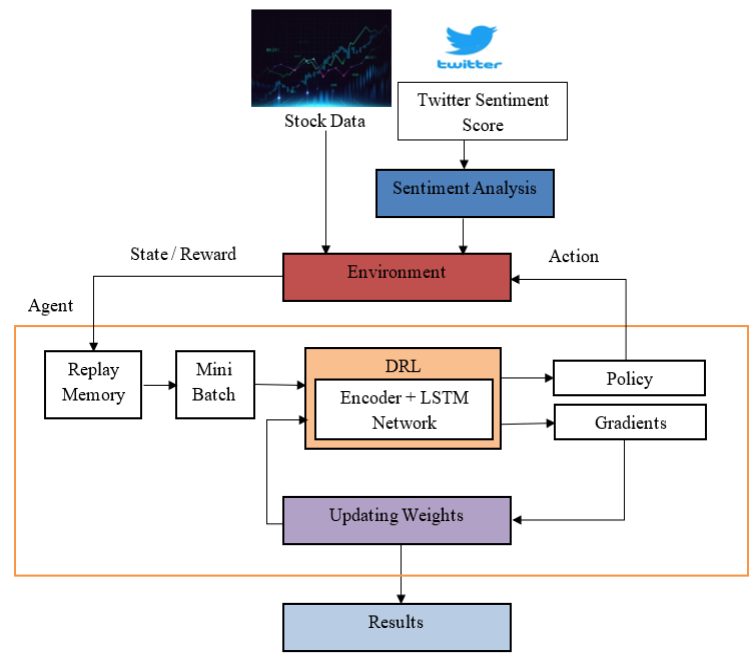
\includegraphics[width=0.55\textwidth]{graphics/2lv4101.png}
    \caption{Proposed framework by \cite{LV41}}
    \label{fig:lv4101}
\end{figure}

Various algorithms are compared: Deep Q-Networks (DQN), Deep Deterministic Policy Gradient (DDPG), Proximal Policy Optimization (PPO), Advantage Actor-Critic (A2C), and their proposed AutoEncoder-LSTM network combined with Reinforcement Learning (AE-LSTM+RL).

The daily closing data of Dow Jones Industrial Average (DJIA) and S\&P 500 data from 2006--2016 are used as training data, and are tested against the real data from 2016--2021. These data are combined with tweet sentiments in the range of [-1,1] calculated from engagement data. Yet, to align with the focus of this thesis, sentiment in this research is not discussed here.

Three benchmarks are used in evaluating the algorithms' performance: 
\begin{enumerate}
	\item Sharpe Ratio: $\frac{R_P-R_B}{\sigma_P}$, where $R_P$ = portfolio return, $R_B$ = benchmark rate, and $\sigma_P$ = standard deviation of portfolio. Penalizes any return below benchmark. Higher is better.
	\item Sortino Ratio: $\frac{R_P-R_B}{\sigma_D}$, where $R_P$ and $R_B$ are identical to above, and $\sigma_D$ = standard deviation of downside. Punishes returns below benchmark within a specific threshold. Higher is better.
	\item Maximum Drawdown (MDD): the maximum percentage of drawdown from the latest portfolio all-time high (ATH). Measures downside risk. Values closer to zero is better.
	\item Annual and cumulative portfolio return (ROI). Higher is better.
\end{enumerate}

The results show that, from the two assets' evaluation, AE-LSTM+RL returns the highest Sharpe Ratio and almost the best Sortino Ratio, annual ROI, and cumulative ROI, yet it causes the highest MDD. A2C performs slightly better or slightly worse to AE-LSTM+RL, PPO's results are often the worst in many benchmarks except it performs best at MDD, DQN and DDPG show similar results to A2C. Results can differ depending on the tested asset or time period, for example, PPO gives the highest annual DJIA return but by far the lowest cumulative return. Hence, supporting \cite{LV91}'s claim regarding the high variability between results given by RL tests, comparing and deciding which conventional algorithm performs the best is not a simple task.

\section{Deep Reinforcement Learning for Trading} %40
Similar to \cite{LV41} but excluding sentiments data and with different assets, Zhang et al. \cite{LV40} compare DQN, Policy Gradients (PG), A2C, with baseline algorithms Long Only, Sign(R), and Moving Average Convergence Divergence (MACD) using nine different metrics to maximize trading portfolio of five asset categories: commodity, equity index, fixed income, foreign exchange, and combined. From the results, DQN yields the best results in most metrics in every investment class except equity index. PG and A2C comparably perform worse than DQN but better than baseline algorithms, with A2C performs better than PG more often.

\section{A2C versus A3C} %compound
Espeholt et al. \cite{LV51} presents one comparison between A2C and A3C as a part of a larger comparison comprising of a proposed novel actor-critic algorithm, batched A2C, and A3C. The focus of the research is not related to trading but to find the most efficient algorithm to learn to complete two puzzles, measured by the training speed and learning outcome. The comparison between A2C and A3C is only found in the single-machine, GPU-less experiment, where A3C with 32 workers and 64 CPUs can process puzzle 1 and puzzle 2 at 6.5K and 9K frames per second (FPS). Meanwhile, batched A2C, 48 CPUs, with step synchronization, can reach 9K and 5K FPS, and batched A2C with trajectory synchronization yields 16K and 17.5K FPS. Again, this comparison is done using different settings and not mentioned in other parts of the study, hence cannot be easily concluded if A2C has any advantage over A3C.

Therefore, a qualitative comparison by Sewak \cite{LV52} between A2C and A3C will be included here. A3C is performed by distributing learning to multiple agents to be done in parallel. Each newly created agent copies the parameters from a centralized network parameter server and trains its data over the parameters. At one time, there will be a merge event where agents combine their own parameters with the global parameter, then replaces each's own parameters with the new global parameter to retrain. However, A3C's asynchronousness can be disadvantageous: agents may have different knowledge of the global state since not every agent pull the global parameters at one time. This is particularly bad if an agent fails or refuses to synchronize with the global parameters for a long time, causing training instability and slower convergence. A2C improves A3C by forcing agents to synchronize at specific times or conditions together at one time. Though, if an agent is unreachable or not responsive, this may cause synchronization delay.

\section{Verdict}
An extensive search of research repositories show that there has not been many, if any, research papers that explicitly compare between conventional algorithms, ML algorithms, and RL algorithms or between A2C against Asynchronous Advantage Actor-Critic (A3C), especially in the applications of trading and portfolio management. Moreover, the comparative results from different existing, or even within the same research, may wildly vary. With similar experiment settings and comparisons, the results can be different, see \cite{LV41} which shows that A2C yields the better results versus \cite{LV40} which clearly signifies that DQN is superior.

\chapter{Background Knowledge}
\label{Background Knowledge}
\indent \indent This chapter introduces concepts and algorithms that are used in this research.

\section{Genetic Algorithm}
\indent \indent Before discussing about genetic algorithms, we visit its hypernym: evolutionary algorithms. Evolutionary algorithms mimic the biological evolution that living beings use to maintain the existence of their species \cite{GA02}: how each generation's lifetime starts and ends and how optimized it performs its ``tasks," compared to other individuals and its parents \cite{GA03}. In evolutary algorithms, ``organisms'' or a model would naturally survive if it has a stronger gene, for example, when it can perform more optimal problem solving capability \cite{GA01}. The keyword ``gene" here introduces us to the concept of ``genetic algorithms."

Genetic algorithms train individual models in a generation to solve a problem: the outcome being trained models and their respective properties (genes), forming a ``gene pool." Each ``genotype'', consists of a set of genes, is represented by a binary string. Only those with higher fitness value can survive and can reproduce in the next training generation. For each iteration, genes from different qualified individuals can recombine with each other or mutate, just like biological gene crossover or mutation \cite{GA01, GA04}. The generational trainings come into when a stop condition has been met.

A classic pseudocode of genetic algorithms is as follows.

\begin{algorithm}
\caption{A Classic Process of Genetic Algorithms \cite{GA05}}
\label{alg-GA}
	obtain initial population\;
	calculate each individual's quality\;
	\While(\tcp*[f]{produce new generation}){not $completed$}{
		\For(\tcp*[f]{recombination cycle}){$population\:size / 2$}{
			choose two individuals to recombine, prioritizing higher quality candidates\;
			recombine the selected two to produce two offspring\;
			calculate each offspring's quality\;
			append the produced individuals into the new generation/iteration\;
		}
		\If{population count converges}{
		{$completed \gets$ TRUE}
		}
	}
\end{algorithm}

\section{Artificial Neural Networks (ANN)}
\indent\indent Artificial Neural Networks (ANN), or in short neural nets (NN), is an interconnected layers of "neurons" that act as processing elements. Connection strength between neurons, which denotes the processing ability of the network, is represented by "weights" \cite{NN01}. ANN is based on the working of living creatures' nervous systems, especially the brain. As concisely aforementioned, a simple NN consists of layers, neurons, and weights, see Fig. \ref{fig:3ann}. In its simplest form, an NN consists of one input layer and one output layer. An input layer can have one or multiple neurons with different values $x_k$ representing the inputted data to the neural network. A weight $w_k$ connects an input neuron $w_k$ and an output neuron $y$ and acts as a multiplier, i.e. the output neuron $y$ will receive the value $w_k{}x_k$ from this connection. A neuron can be a source of multiple weights to the next layer and also a destination of multiple weights from the previous layer. The value of a output layer neuron in Fig. \ref{fig:3ann} is equal to $y = f(\sum^{n-1}_{i=0}w_i{}x_i-\theta)$, where $f$ is an activation function, e.g. Sigmoid, normalization, etc. and $\theta$ an internal threshold or offset. Lastly, the output layer, after receiving its final value, becomes the output of the NN. An output layer is useful for classification problem: it shows which neurons have a value that lies within a specific classification threshold.

\begin{figure}[h]
    \centering
    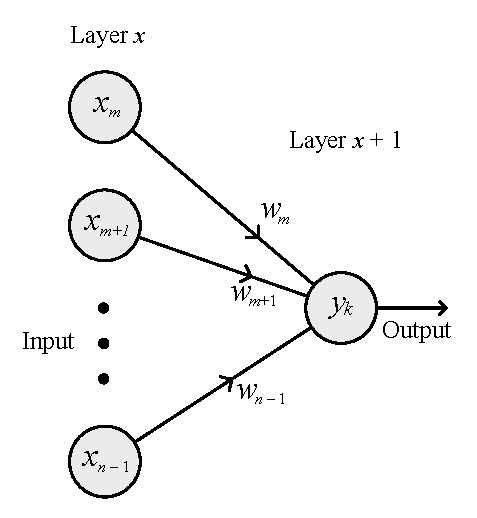
\includegraphics[width=0.35\textwidth]{graphics/3ann.pdf}
    \caption{Structure of an ANN \cite{NN01}}
    \label{fig:3ann}
\end{figure}

The correctness or quality of an ANN can be determined using a loss function, which indicates the disparity between the expected output and the prediction produced by the ANN. Loss function may also be used to adjust other hyperparameters, such as weights \cite{NN02}.

%/parameter, hyperparameter
%/construction
%/loss fn etc
%/prediction
%/tuning/optimization
%/uses

\subsection{Deep Learning}
Deep learning improves ANN in a way that it is multi-layered: each layer processes different levels of features. Deep learning algorithms have intermediary layers between the input and output layers which in a progression extract useful input patterns and pass them to the subsequent layer \cite{NN03}. According to how inputs are presented or obtained, deep learning can be divided into multiple types, most prominently (1) supervised learning, (2) unsupervised learning, (3) reinforcement learning, or (4) combination between any of (1), (2), or (3).

Supervised learning problems has the following characteristics. First, data is presented in the form of $X \mapsto Y$, where $X$ is a representation data labeled with a label $Y$. Next, the learning agent will abstractly learn the relations between $X$ and $Y$ as a knowledge base to predict the label of a new input. Unsupervised learning lacks $Y$ part such that the learning agent needs to infer data classification from the feature distribution of input data. Agents in reinforcement learning learns independently, assisted from rewards and punishments from performing an action in one environment state.

\section{Analytic Trading}
\indent\indent Trading, in this sense, refers to an activity of buying, selling, or holding a commodity, stock, currency, or other derivative assets in their corresponding finacial markets. The ultimate goal of trading is to gain profit from price difference and minimizing transactional cost. Analytic trading optimizes profit-making decisions by predicting price actions based on fundamental analysis plus chart features such as price trend, support and resistance levels, trading volume, trading indicators, price patterns, etc. \cite{AT52}. Fig. \ref{fig:3tv} shows Bitstamp's Bitcoin-USD pair chart taken from TradingView on 5 August 2022, at 9:01 AM UTC. It contains different indicators: Volume (Vol), Moving average with window size equals 28 bars (MA(28)), MACD long/short strategy, and Bollinger Bands with window size 20 and band deviation of 2 sigma (BB(20,2)).

\begin{figure}[h]
    \centering
    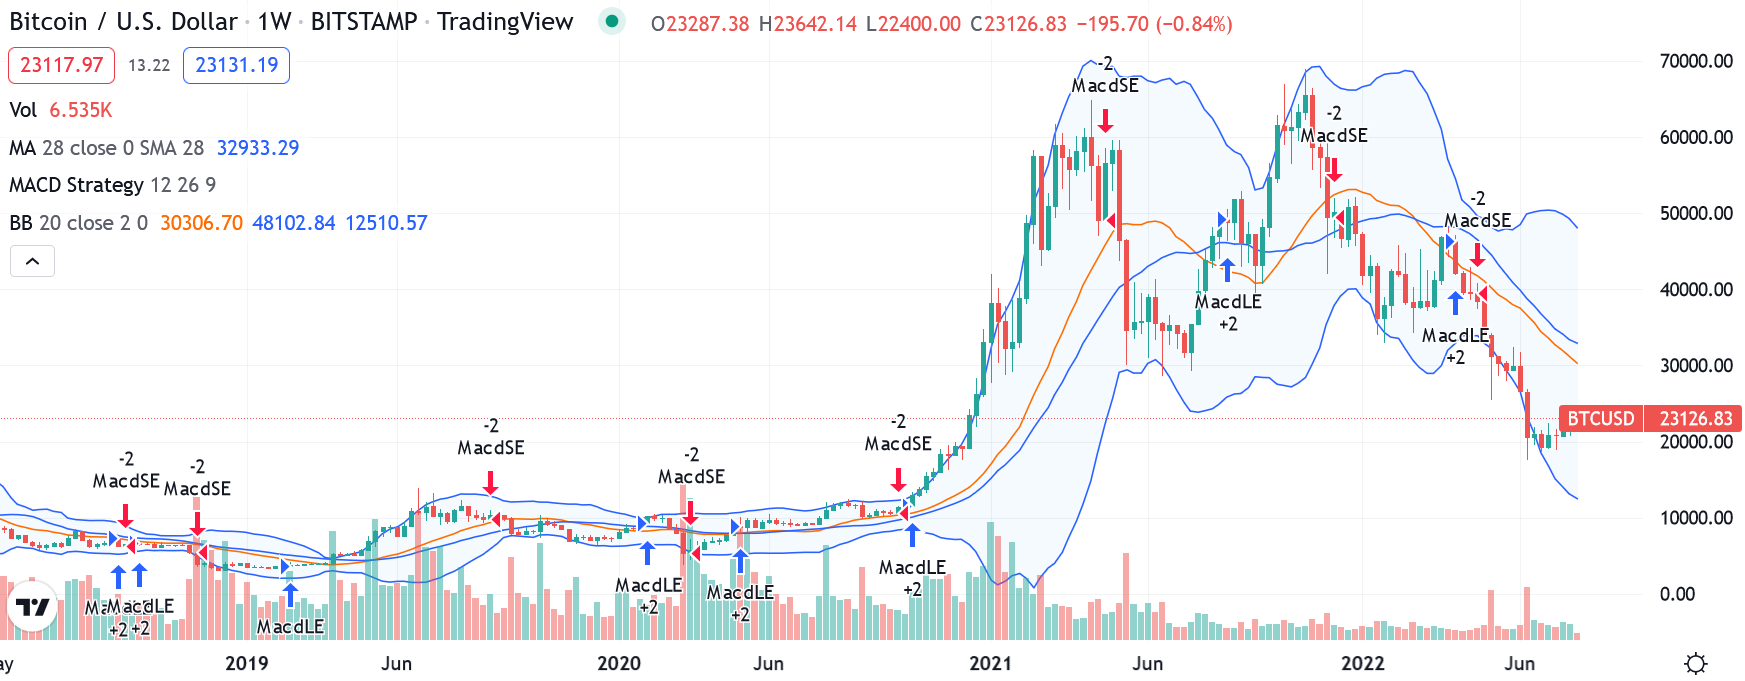
\includegraphics[width=0.96\textwidth]{graphics/3bitcoinindicators.png}
    \caption{An example of trading chart with several indicators \cite{X001}}
    \label{fig:3tv}
\end{figure}

Typically, the input data of a price prediction problem is in a form of a time series data \cite{AT51}. Values from a time window is then calculated and analyzed to obtain various indicators to assist trading decision. More recent approaches automate trading decisions in a form of algorithmic (algo) trading, which can generate decisions in (near-)real time. Sometimes, algo trading is empowered by artificial intelligence and ANN to improve the prediction performance as well \cite{AT49}.

Many fund managers nowadays have shifted their interest to trade cryptocurrencies due to their profit-inducing volatility \cite{AT72} and rapid development \cite{AT71}. Bitcoin, being the first invented and the most mature cryptocurrency, has become the cryptocurrency standard in various researches and studies \cite{AT72}.

There are three basic actions in spot trading: \texttt{Buy}($x$) or \texttt{Long}, \texttt{Sell}($x$) or \texttt{Short}, and \texttt{Hold}. \texttt{Buy}($x$) tells the trading bot to buy $x$ units of asset at the specified time, \texttt{Sell}($x$) works similarly but for selling, and \texttt{Hold} is to neither buy nor sell the asset at the specified time point. Decision to choose one of the three depends on indicators, or in ANN-enhanced decision, the output of the ANN.

This research uses two popular indicators: exponential moving average (EMA) and Moving Average Convergence/Divergence (MACD), a derivative of EMA. $EMA$($x$) is defined as
\[
	EMA(x) = p \cdot k + EMA_p \cdot (1 - k),
\] where $n = \frac{2}{x+1}$, $x$ is the number of time frames considered in the EMA, $p$ is the asset price at the current timeframe, and $EMA_p$ is the value of EMA of the previous day \cite{AT22}. Since the function is recursive, the base case of the formula, for the first datapoint, is \cite{AT23}
\[
	EMA_0(x) = \frac{\sum_{i=0}^{t - 1} p_i(1-\alpha)^i}{\sum_{i=0}^{t-1}(1-\alpha)^{i}},
\] where $\alpha$ is the discounting factor of past values, typically is 0.18.

MACD, on the other hand, uses EMA in its calculation, and is defined as: $MACD(f, s)$ = $EMA(f) - EMA(s)$. $f$ stands for ``fast" moving average, typically is fixed at 12. $s$ is ``slow" moving average, typically is equal to 26. On top of that, $EMA(l)$ of $MACD$ is called the ``signal line", equals to $EMA(l) - MACD(f, s)$ \cite{AT23}. Signal line (hereafter notated by $\sigma$) is useful to trigger buy and sell signals. When $MACD - \sigma$ turns from negative to positive, a buy signal is issued; when it turns from positive to negative, a sell signal is issued. Otherwise, no trade is done.

\subsection{Deep Learning for Trading}
\label{sec:dl}
Long-Short Term Memory (LSTM), a subset of Recurrent Neural Network (RNN), is a popular supervised deep learning algorithm for trading bots since its nature fits with predicting future values from past data. This class of RNN uses either sigmoid or hyperbolic tangent (tanh) activation function and SoftMax. Back propagation in RNN, when seeing a non-optimal result, may redirect the outputs of the network to the hidden, intermediary layer, in a hope to improve the prediction result \cite{AT20}.

LSTM improved long-term forecasting by adding more memory into RNN. Each LSTM `cell' (Fig. \ref{fig:3lstm} \cite{NN05}) has two states: hidden state ($h$, to process input and output and short-term memory) and cell state ($c$, for data flow and long-term memory). There are several steps in building an LSTM network \cite{NN04}. First, forgetting unused information from previous step ($h_{t_1}$) and input $X_t$ using a sigmoid function ($\sigma$) through the forget gate ($f_t$, a vector whose values are between 0 and 1). The next stage is remembering new information from $X_t$ through the memory gate ($i_t$ to accept or discard new information multiplied by $\tilde{C}_t$ to give an importance level to the input). Finally, the output of the cell $h_t$ is obtained by multiplying $\sigma(h_{t_1})$ and $c_t$.

\begin{figure}[h]
    \centering
    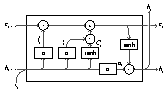
\includegraphics[width=0.48\textwidth]{graphics/3lstm.pdf}
    \caption{An LSTM cell}
    \label{fig:3lstm}
\end{figure}

LSTM, in this regard, however, is used mostly for forecasting stock prices. Trading decisions are generated using another deep learning algorithm called Convolutional Neural Network (CNN). CNN, usually used for feature extraction in multidimensional spaces like images, learns stock movement patterns (trend, trajectory) and thus can decide when to buy or sell an asset \cite{AT21}. Not many works indicate the ROI, but prediction accuracy. Yet, Chakole and Kurhekar's work \cite{AT21} show that a plain CNN would return a lower ROI than other methods, including the buy-and-hold method.

\section{Markov Decision Process (MDP)}
\indent\indent Markov Decision Process is central to the main concept of this research Reinforcement Learning (RL). MDP mimics the working of decisions in human life, focuses on choosing the better impact from decisions. MDP can be modeled after a finite state machine like in Fig. \ref{fig:3mdp}. An agent can choose to go from a state to another state (or back to its current state) via an action and receive a reward for each state propagation. In a more general definition, an agent can act upon the environment to move to another state and receive a reward as a consequence \cite{ML01}.

\begin{figure}[h]
    \centering
    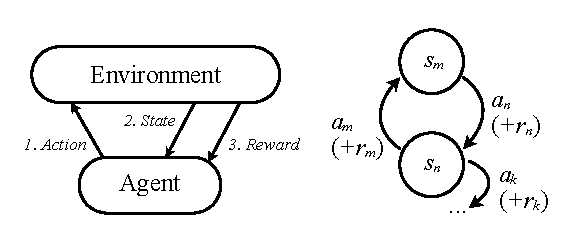
\includegraphics[width=0.66\textwidth]{graphics/3mdp.pdf}
    \caption{Markov Decision Process in two views.}
    \label{fig:3mdp}
\end{figure}

The formulation of MDP is as follows \cite{ML01}:

\[
r_t(s,a)=\sum_{s'\in{}S}r_t(s,a,s')p_t(s'|s,a),
\]

where $r$ denotes reward, $t$ is the current propagation instance, $r_t(x)$ is the reward of performing a propagation $x$, $s$ is the current state, $a$ indicates the action taken, $s'$ is the next state after performing $a$ on $s$, and $p(x)$ is the probability of propagation with condition $x$ happening.

According to Feinberg and Schwartz \cite{BK01}, there are two kinds of impacts: (1) cost minimization and profit maximalization and (2) impacts on future states after the decision. MDP looks for a decision that is profitable in long-term period by choosing optimal policies. MDP is shown to be useful in various implementations. In finance and investment, \cite{BK03} uses MDP to decide when to sell or hold a financial asset to get faster gain. Saario \cite{BK04} tries to solve a house-selling problem, that is, someone must decide to sell a house given an arbitrary offer or decline the offer and wait longer for a better offer. An MDP-like dynamic programming (DP) solution is used to maximize the accepted offer value.

\subsection{Bellman Equation and Optimality}
% Bellman, Bellman optimality
Bellman equation plays an important role in dynamic programming: it expects the total reward from the present state $s$ to the end of the propagation horizon in an MDP. The equation \cite{ML01} is as follows:

\[
v^{\pi}_t(s) = \max_{{a\in{}A(s)}}\left\{r_t(s,a)+\sum_{s'\in{}S}\gamma^t p(s'|s,a)v_{t+1}(s')\right\},
\]

where $v^{\pi}_t(s)$ is the expected present and future total rewards from the current state $s$. A discounting factor $\gamma^t$, $0 < \gamma < 1$ is sometimes added to diminish the effect of far-future rewards and to put priority to near-future rewards.

The best and most optimal possible $v^{\pi}_t(s_0)$ is denoted by $\max_{\pi}v^{\pi}(s) = v*(s)$. Bellman's Optimality Theorem states that \cite{BK05} $v^*(s)$ must satisfy the Bellman Optimality Equation
\[
	v^*(s)=\max_{a}\left\{r(s,a)+\gamma{}\sum_{s'}p(s'|s,a)v^*(s')\right\}
\] for all $s$.

\section{Reinforcement Learning (RL)}
\indent\indent Reinforcement Learning (RL), a branch of deep learning, is analogous to how living things learn to perceive and to interact with their environment: by doing something experimentally then receiving a reward or a punishment as a consequence \cite{RL01}. Like so, RL iteratively learns causes and effects under little supervision to reach the goal of obtaining as much reward as possible, in a computational way.

Based on finite MDP, RL can be illustrated using Fig. //ADD FIGURE HERE// \cite{RL01}. Five elements of RL are :
\begin{enumerate}
	\item Agent: the entity which learns about the environment by taking actions and receiving rewards,
	\item Environment: every entity other than the agent whom the agent interacts with,
	\item State $S_t$: the current state or constellation of the environment,
	\item Action $A_t$: a set of tasks or actions that the agent can take at the current state to change the state of the environment, and
	\item Reward $R_t$: the consequence that the agent receives upon completing an action.
\end{enumerate}

\subsection{Policy in RL}
The output of RL is a policy $\pi_t$ for each time step, that is, $\pi_t(a|s)$, a probability of choosing an action $A_t = a$ given the current state $S_t = s$. The ultimate goal is to produce a set of policies $\pi_t$ for every $A_t$, $S_t$ which maximizes $R_t$ in the long run. In an equation \cite{QL03},

\[\pi^* := \argmax_x \mathbb{E} \left[ \sum_{k=0}^{\infty} \gamma^k{}r_k \middle| \pi \right],\]

where $\pi^*$ is a deterministic optimal policy, $\mathbb{E}[\cdot|\pi]$ is expectation based on policy $\pi$, $\gamma$ is discount factor, which determines agent's consideration of possible future actions. $\pi$ itself describes the policy under a state-action trajectory $s_0, a_0, s_1, a_1, ..., a_{k-1}, s_k$.

\subsection{RL Taxonomy}
The following list adopted from \cite{RL07} shows the taxonomy of RL algorithms. Some of the subbranches and algorithms will be discussed in the subsequent paragraphs.

\begin{enumerate}
	\item Model-Based RL
	\begin{enumerate}
		\item Model given, e.g., \texttt{MCTS} (Monte Carlo tree search)
		\item Model learned, e.g., \texttt{I2A} (Imagination-Augmented Agents), World Model
	\end{enumerate}
	
	\item Model-Free RL
	\begin{enumerate}
		\item Value-Based: focus on state-action value
		\begin{enumerate}
			\item On-Policy: policy determines learning
			\begin{itemize}
				\item \texttt{Sarsa}
			\end{itemize}
			\item Off-Policy: learning is done randomly
			\begin{itemize}
				\item \texttt{Q-Learning}
				\item \texttt{DQN} (Deep Q-Network), 
				further classified into \texttt{C51},
				\texttt{Dueling DQN}, \texttt{Double DQN}, \texttt{QT-Opt},
				and \texttt{DDPG} (Deep Deterministic Policy Gradient).
			\end{itemize}
		\end{enumerate}
		\item Policy-Based: focus on overall policy value
		\begin{enumerate}
			\item Gradient-free
			\begin{itemize}
				\item Cross-Entropy Method: \texttt{QT-Opt} (intertwined with \texttt{DQN})
				\item Evolution Strategy: \texttt{SAMUEL}
			\end{itemize}
			\item Gradient-based
			\begin{itemize}
				\item \texttt{Policy Gradient}
				\item \texttt{TRPO/PPO} (Trust Region Policy Optimization/Proximal Policy Optimization)
				\item \texttt{ACKTR} (Actor Critic using Kronecker-Factored Trust Region)
				\item Actor-Critic
				\begin{itemize}
					\item \texttt{A2C} (Advantage Actor Critic)
					\item \texttt{A3C} (Asynchronous Advantage Actor Critic)
					\item \texttt{DDPG} (Deep Deterministic Policy Gradient), combined with \texttt{DQN}: \texttt{TD3} (Twin Delayed DDPG), \texttt{SAC} (Soft Actor Critic)
				\end{itemize}
			\end{itemize}						
		\end{enumerate}
	\end{enumerate}
\end{enumerate}

\subsubsection{Model-based and Model-free Reinforcement Learning}

A model in RL refers to any data or knowledge that contains the state-action-reward prediction table for an agent to plan and follow. Model-based RL uses a model, learned or known, and approximates a policy function from learning \cite{RL04}. Model-free RL, on the other hand, calculates the environment spontaneously using trial-and-error, while retaining no transition probability distribution arrays, hence learning how to act solely based on rewards \cite{RL05}. Model-free algorithms are viewed to be labor-intensive but can adapt to new environment fast, while model-based algorithms are more lightweight but produce less optimal policies, hence are more suitable for deterministic use cases.

\subsubsection{Actor-Critic Method}
Konda and Tsitsiklis \cite{RL06} observe that most RL algorithms are either actor-only or critic-only. Actor-only methods focus on parametrization of policies and parameter improvisation without learning process. An example of actor-only methods is REINFORCE. Critic-only methods use solely value approximation in learning to comply with the Bellman equation, but produce less optimal policy. An example of critic-only methods is Q-learning.

Thus, the actor-critic method is derived to fuse the advantages of actor-only and critic-only algorithms. Actor-critic mathods typically use two separate neural networks: a neural network for actor and a neural network for critic \cite{RL101}. The critic part approximates and simulates learning to improve the actor segment's policy parameters.

\subsubsection{Policy Gradient}
% grad descent explained in short only
Actor-critic algorithms often use the policy gradient theorem \cite{RL07}. However, Sutton et al. \cite{RL27} claim that sole function approximation is not effective enough in realizing a policy convergence. One effort is to parametrize the policy instead of computing the policy from parametrized action-value functions. This way, one can track and plan the gradient descent of the overall policy parameter. Say that the policy parameter is denoted by $\theta$, the gradient $\Delta\theta = \alpha\hat{\nabla}_\theta{}J(\theta)$ can be adjusted by setting $\alpha$: step size and $J(\theta)$: RL performance of the policy that follows the parameter $\theta$, either calculated by total reward or reward per step.

\paragraph{Gradient Descent}
Gradient descent itself is a method that iteratively minimize a function value. Imagine a function $y = f(x_1, x_2, ..., x_n)$. Gradient descent starts with choosing a random or predefined parameter vector $x_1, x_2, ..., x_n$ as the initial position. Obtain the gradient vector by observing the change of $y$ when each of $x_1, x_2, ..., x_n$ is changed by a little. Next, adjust some $x$ using a predefined step to get $y$ with smaller value and repeat until a local minima for $y$ is found. This process can be illustrated by Fig. \ref{fig:3gdes}.

\begin{figure}[h]
    \centering
    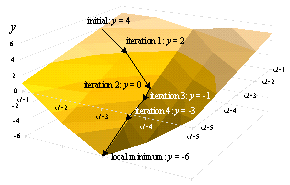
\includegraphics[width=0.66\textwidth]{graphics/3gdes.pdf}
    \caption{Gradient descent}
    \label{fig:3gdes}
\end{figure}

\subsubsection{Q-learning}
\label{qlearning-dqn}
Q-learning is a model-free RL algorithm which explores the maximum reward of all possible state-action propagations, updated for every propagation. The Q-function $Q(s,a)$ is defined as $r(s,a)+\gamma{}v^*(\delta(s,a)) = r(s,a) + \gamma \max_{a'} Q(\delta(s,a),a')$, where $\delta$ is a state transition function. Therefore, in Q-learning notation, $\pi^*(s) = \argmax_{\pi} Q(s,a)$. The maximum current rewards of state-action pairs are recorded in an $n-$dimensional array, and for each iteration, Q-learning will choose the action with the highest reward, based on the current state. The algorithm is as follows \cite{RL01}:

\begin{algorithm}
\caption{Q-learning Algorithm}
\label{alg-QL}
	$Q(s,a), \forall s \in S, a \in A(s) \gets$ an arbitrary value\;
	$Q(terminal\:state, \cdot) = 0$\;
	\While{$S$ is not terminal state}{
		$S gets$ initial value\;
		\For{each propagation}{
			Based on $\pi$ constructed in $Q$, select possible $A$ for the current $S$\;
			Perform $A$, get $R$ and $S'$\;
			$Q(S,A) \gets Q(S,A) + \alpha[R + \gamma \max_{a}Q(S',a)-Q(S,A)]$
			$S\gets S'$
		}
	}
\end{algorithm}

\paragraph{Q-learning with Deep Learning}
However, in a system with huge dimensions of $A$ and $S$, calculating $Q$ value for all $S,A$ pairs consumes heavy resources which is unsustainable and inefficient. Mnih et al. \cite{RL03} combine Q-learning with Deep Learning, called a deep Q-network (DQN), to convert high-dimensionality input into a quantized, pattern-matched inputs with lower dimensionality. The work gives an example scenario: an RL agent needs to observe a video game with 84 $\times$ 84 $\times$ 4 consecutive images $\times$ 256 grayscale levels and to act upon the state by ``clicking" on one of many controller buttons. With a plain array-based Q-learning, each state change require the system to recursively calculate $256^{84 \times 84 \times 4} \times 18 \approx 10^{69971}$ Q values, assuming that there are at most 18 different actions that the agent can take. That value exceeds the number of atoms in the universe, which is $\approx 10^{82}$. With DQN, state-action-reward mappings are approximated using convolutional neural network on-the-go and per-request. This way, determining action would not require storing or generating much, and sometimes unnecessary, prior knowledge.

\subsection{This Research's RL Algorithms in A Nutshell}
Alongside with DQN which is introduced in Section \ref{qlearning-dqn}, four RL algorithms are used: Asynchronous Advantage Actor Critic (A3C), Advantage Actor Critic (A2C), Soft Actor-Critic (SAC), and Proximal Policy Optimization (PPO).

\subsubsection{Asynchronous Advantage Actor Critic (A3C) and Advantage Actor Critic (A2C)}
A3C came from a research by Mnih et al. \cite{RL103} that proposes an asynchronous deep RL framework which adds asynchronous, parallel actor-learners over Sarsa, one-step Q-learning, n-step Q-learning, and A2C. The framework is designed such that multiple RL actor-learners are run in different CPU threads, updating a centralized parameter server. The work finds that parallel workers expand the exploration horizon, hence maximizes knowledge procurement and thus learning speed. Among the asynchronized versions of the four base algorithms, asynchronous A2C (thus called A3C) is the fastest agent that reaches the higher score when tested on Atari 2600 games.

A2C, derived in the same work, is a version of A3C with only one agent. In short, A2C is an improvement of vanilla actor-critic method with an addition of \textit{advantage} value: how advantageous it is to take an action $a_t$ compared to the average of all possible actions at the state $s_t$ \cite{RL103W}.

\subsubsection{Proximal Policy Optimization (PPO)}
OpenAI's Schulman et al. \cite{RL102} derived a family of algorithms called the Proximal Policy Optimization (PPO) algorithms, a subset of policy-based RL. PPO improves Trust Region Policy Optimization (TRPO) in terms of implementation, sample complexity, and execution time. For one eposide of policy update, PPO goes through multiple or batched small episodes of stochastic gradient policy ascent. Moreover, PPO focuses on the area of policy gradient change with high probability, to increase policy faster and more efficiently. Tested using benchmark RL tasks (\texttt{Hopper-v1}, \texttt{Walker2d-v1}, \texttt{HalfCheetah-v1}, etc.), PPO is claimed and shown to perform better than A2C, CEM, TRPO, A2C with Trust Region, and vanilla Policy Gradient method.

\subsubsection{Soft Actor-Critic (SAC)}
An example actor-critic algorithm that combines policy-based and value-based RL is Soft Actor-Critic (SAC) \cite{RL100}. SAC optimizes policy function using an off-policy way by mimicking Q-Learning's approach to accomplish a task: by acting balancedly random (maximizing entropy) yet also enhancing expected reward. The original work \cite{RL100} indicates that SAC performs better on benchmark RL tasks (\texttt{Hopper-v1}, \texttt{Walker2d-v1}, \texttt{Ant-v1}, etc.) compared to prior works such as TD3, DDPG, PPO, and Soft Q-Learning (SQL).
\chapter{Methodology}
\label{methodology}

This research considers seven trading methods to be compared: \textbf{buy-and-hold}, \textbf{MACD} indicator trading, two value-based model-free RL algorithms \textbf{DQN} and \textbf{Sarsa}, two policy-based model-free RL algorithms \textbf{A2C} and \textbf{A3C}, and one model-based RL algorithm \textbf{PETS}.

\section{Dataset}
All training and testing data \texttt{BTC} data in term of \texttt{USD}. A sole training dataset $\mathcal{D}_{train}$ is fetched from CryptoDataDownload \cite{DATA01}, containing 11,144 per-hour data points from to 14 October 2020 22:00 UTC to 22 January 2022 05:00 UTC. This date range is selected because it is a crab market with two bull markets and two bear markets.

Test datasets $\mathcal{D}_{test}$ are provided by Cryptocompare\footnote{https://www.cryptocompare.com/} API, consists of two sets of timeframes, namely:
\begin{itemize}
	\item Each-hour bull data (\texttt{HBu}): 2,000 points of data from 9 November 2022 06:00 UTC to 31 January 2023 14:00 UTC inclusive,
	\item Each-hour bear data (\texttt{HBr}): 2,000 points of data from 9 November 2021 06:00 UTC to 31 January 2022 14:00 UTC inclusive,
	\item Each-minute crab data (\texttt{MCr}): 2,000 points of data from 16 February 2023 04:40 UTC to 17 February 2023 14:00 UTC inclusive,		
	\item Each-minute bull data (\texttt{MBu}): 2,000 points of data from 14 February 2023 04:40 UTC to 15 February 2023 14:00 UTC inclusive.
\end{itemize}

Each data point contains five information:
\begin{itemize}
	\item \texttt{timeframe}: the time point where the price movement occured,
	\item \texttt{high}: the highest price recorded in that timeframe,
	\item \texttt{low}: the lowest price recorded in that timeframe,
	\item \texttt{open}: the price recorded at the start of that timeframe,
	\item \texttt{close}: the price recorded at the end of that timeframe.
\end{itemize}

The datasets go through a preprocessing step that adds three more custom columns to the original data, namely:
\begin{itemize}
	\item \texttt{ewm}: the value of $EMA(28)$ of that timeframe,
	\item \texttt{macd\_histo}: the values of $MACD(26,12,9) - SignalLine$ of that timeframe,
	\item \texttt{return}: the price movement since the last data point's close.
\end{itemize}

\section{Problem Representation}
Given a dataset $\mathcal{D}$ and an initial investment of \texttt{USD 10,000}. At each data point $d_t$ at timeframe $t$, a trading agent must decide to perform an action: either \texttt{BUY}, \texttt{SELL}, or \texttt{HOLD}. Since the setting is a spot trading environment, the agent is not allowed to buy more asset than its current unspent capital and is not allowed to sell more than the value of Bitcoin it holds. All trades are executed without transaction fees, following Binance's move\footnote{https://www.binance.com/en/support/announcement/binance-launches-zero-fee-bitcoin-trading-10435147c55d4a40b64fcbf43cb46329}. Finally, all agents are compared against another using the factors specified in Section \ref{sec:performancemx}.

\section{Performance Metrics}
\label{sec:performancemx}
Three performance metrics are used for final agent evaluation and also act as factors that determine reward\footnote{however, see \ref{rewardfn}}:
\begin{itemize}
	\item The average of portfolio return of agent $\alpha$ at all timeframes ($\phi_\alpha$) over benchmark return ($\phi_\odot$) = $average(\phi_\alpha - \phi_\odot)$, symbolized as $\overline{\Delta\phi_{\alpha,\odot}}$: larger is better,
	\item Maximum drawdown at the final timeframe $T$ (MDD$_T$): ranges from 0 to 1, closer to zero is better, and
	\item Non-annualized 100-timeframe Sortino ratio at the final timeframe $T$ ($\zeta_T$), larger is better.
\end{itemize}

To compare between agents, in addition to the above factors, one extra factor is included: 
\begin{itemize}
	\item Training speed ($s$), calculates the approximate time it takes for the training reward to converge in seconds, smaller is better. The number of episodes at the time point may follow.
\end{itemize}

\section{Non-RL Agents}
% how to perform the experiment
% Buy-and-Hold, MACD, RL algo in detail (implementation)
\subsection{Buy-and-Hold Agent}
The buy-and-hold agent is the bare basic agent as a global control variable, usually called as the ``benchmark" in algo trading. The strategy is simple: buy at the first timeframe and sell at the last timeframe. There is no learning or calculation involved. Directly using testing datasets, the portfolio return (as a ratio) of this agent is equal to $\frac{p_{2000} - p_0}{p_0}$, in other words, the price movement relative to the initial price. An agent can be called a profitable agent if and only if it can perform better than this benchmark.

\subsection{MACD Strategy Agent}
The MACD strategy agent follows the signal from \texttt{macd\_histo} to decide when to buy, when to hold, and when to sell. This agent acts as a second benchmark, representing simple statistical trading agents. The agent can only buy or sell the asset using all its capital: no order splitting is performed here. Therefore, directly using the four testing datasets, the portfolio return of the MACD strategy agent is $\frac{\phi_{2000}}{\phi_0}$, where $\phi_t = \phi(USD)_t + rate_t \times \phi(BTC)_t$: the total portfolio in both \texttt{USD} and \texttt{BTC}.

\section{RL Agents}
This section describes the design of the trading agent: action space, state space, and the reward function. There are eight types of agents that share the same RL agent class, namely: DQN-discrete, A2C-continuous, A2C-discrete, PPO-continuous, PPO-discrete, SAC-continuous, A3C-continuous, and A3C-discrete.

\subsection{Agent Characteristics}
Table \ref{tab:std_hyperparameters} shows the characteristics and hyperparameters used for each algorithm.
% Please add the following required packages to your document preamble:
% \usepackage{longtable}
% Note: It may be necessary to compile the document several times to get a multi-page table to line up properly
\begin{longtable}[c]{|c|ccccc|}
\caption{Agent Characteristics and Hyperparameters}
\label{tab:std_hyperparameters}\\
\hline
 & \multicolumn{1}{c|}{\textbf{DQN}} & \multicolumn{1}{c|}{\textbf{PPO}} & \multicolumn{1}{c|}{\textbf{A2C}} & \multicolumn{1}{c|}{\textbf{SAC}} & \textbf{A3C} \\ \hline
\endfirsthead
%
\multicolumn{6}{c}%
{{\bfseries Table \thetable\ continued from previous page}} \\
\endhead
%
\textbf{Discount factor ($\gamma$)} & \multicolumn{5}{c|}{0.99} \\ \hline
\textbf{Learning rate} & \multicolumn{1}{c|}{0.0001} & \multicolumn{1}{c|}{0.0003} & \multicolumn{1}{c|}{0.0007} & \multicolumn{1}{c|}{0.0003} &  \\ \hline
\textbf{Network type} & \multicolumn{4}{c|}{2-layer fully-connected CNN} &  \\ \hline
\textbf{Actor-Critic net} & \multicolumn{1}{c|}{-} & \multicolumn{2}{c|}{shared} & \multicolumn{1}{c|}{separate} &  \\ \hline
\textbf{Neurons per layer} & \multicolumn{1}{c|}{64} & \multicolumn{1}{c|}{64} & \multicolumn{1}{c|}{64} & \multicolumn{1}{c|}{256} &  \\ \hline
\textbf{Number of episodes} & \multicolumn{1}{c|}{200} & \multicolumn{1}{c|}{200} & \multicolumn{1}{c|}{150} & \multicolumn{1}{c|}{150} & 200 \\ \hline
\textbf{Action space} & \multicolumn{1}{c|}{discrete} & \multicolumn{1}{c|}{\begin{tabular}[c]{@{}c@{}}discrete,\\ continuous\end{tabular}} & \multicolumn{1}{c|}{\begin{tabular}[c]{@{}c@{}}discrete,\\ continuous\end{tabular}} & \multicolumn{1}{c|}{continuous} & \begin{tabular}[c]{@{}c@{}}discrete,\\ continuous\end{tabular} \\ \hline
\textbf{Library} & \multicolumn{4}{c|}{Stable-Baselines3} & Machin \\ \hline
\textbf{Other factors} & \multicolumn{1}{c|}{\begin{tabular}[c]{@{}c@{}}Exploration:\\ initial rate = 1,\\ decay rate = 0.1,\\ final rate = 0.05\end{tabular}} & \multicolumn{1}{c|}{clip range = 0.2} & \multicolumn{1}{c|}{} & \multicolumn{1}{c|}{} &  \\ \hline
\end{longtable}

\subsection{Action Space}
There are two types of action state: continuous and discrete. 

\paragraph{Continuous Action Space}
Trading with continuous action space allows the bot to perform a trade only using a certain amount of portfolio (in portion), e.g., buy BTC using 15\% of available balance, etc. The continuous action space is a two-dimensional array consisting of \texttt{action\_type} and \texttt{action\_percentage}. The range of \texttt{action\_type} is [0,3), where [0,1) triggers the \texttt{BUY} signal, [1,2) for \texttt{SELL} signal, else \texttt{HOLD}. And \texttt{action\_percentage}, ranging at [0,1], indicates the amount of portfolio to trade (buy/sell) with. \texttt{action\_percentage} has no effect on \texttt{HOLD} action.

There are some additional constraints to make: to limit the number of buys and sells, the agent can only perform a \texttt{BUY} when the amount to buy is more than 0.001 BTC and there is at least USD 100 to spend. Moreover, the agent can only \texttt{SELL} when the trade size is over 0.001 BTC and the amount held is more than 0.0001 BTC.

\paragraph{Discrete Action Space}
Trading with discrete action space allows the bot to perform a trade only using the whole portfolio balance. The discrete action space is a scalar with three possible values: 0 for \texttt{BUY}, 1 for \texttt{SELL}, and 2 for \texttt{HOLD}. This mode also employs the exact same constraints like in the continuous action space.

\subsection{State Space}
The observable state space is in the continuous space, consists of the past five values of {\texttt{return}}, which is a stationarized data. An alternative case would be including the movement of \texttt{macd\_histo} and \texttt{ewm}, but after several observations, the final reward would perform randomly, poorly, or never converge. Refer to Figs. \ref{fig-three-bad} as a reference.

\begin{figure}[h]
    \centering
    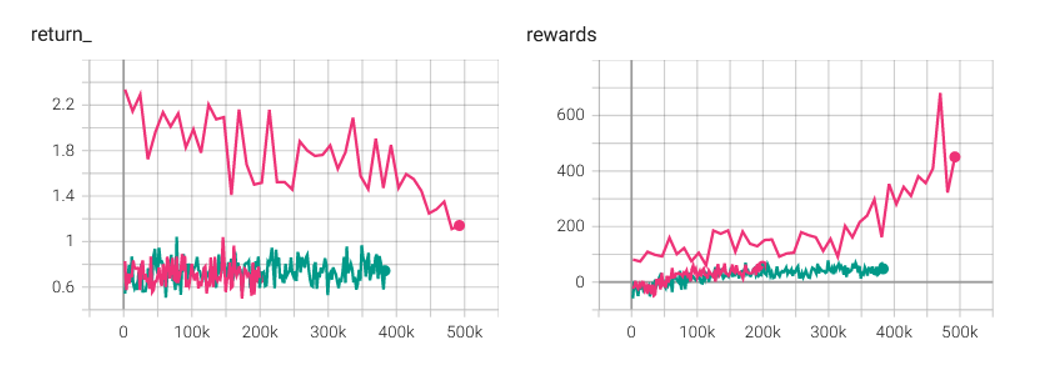
\includegraphics[width=0.79\textwidth]{graphics/fig-three-bad.png}
    \caption{Rewards and returns (PPO) when using state space with three values. The declining pink line in \texttt{return\_}, corresponds to the upper pink line in \texttt{reward}, appeared when Sortino is involved in reward calculation. The $x$-axis indicates the number of timesteps of learning.}
    \label{fig-three-bad}
\end{figure}

\subsection{Reward Function}
	\label{rewardfn}
The reward function for both continuous and discrete action spaces is described using Algorithm \ref{algoreward}.

\begin{algorithm}[h]
\SetAlgoLined
\KwIn{action type}
\KwOut{reward}

\eIf{action = \texttt{BUY}}{
reward $\leftarrow$ 0;
}{
\eIf{action = \texttt{SELL}}{
$reward\_profit \leftarrow sold\_amount \times (sell\_price - average\_held\_price) / average\_held\_price$ \;
$reward\_mdd \leftarrow (latest\_mdd - current\_mdd) \times 0.5$ \;
$reward \leftarrow reward\_profit + reward\_mdd$ \;
}{
$reward\_profit \leftarrow hold\_amount \times (0.0001 * (net\_worth - initial\_balance) / initial\_balance) - 0.0001$ \;
}
}

\KwRet{reward}
\caption{Reward Calculation Algorithm}
\label{algoreward}
\end{algorithm}

There is no reward for buying. Multiplied by the holding amount, holding costs 0.0001 parts of profit or loss added with a flat -0.0001 points of reward to avoid lazy trading: a condition where the agent becomes hesitant to trade to avoid loss, plus a small amount of reduction when the unrealized profit is in the negative zone. When selling, two kinds of rewards are added together. The first component is profit reward, which is the difference between the selling price and the average holding price relative to the average holding price. The last component is how much MDD increases after the selling action times 0.5 to give it less priority than profit reward. The two components are multiplied by the selling amount.

Like determining state space and also mentioned in Fig. \ref{fig-three-bad}, Sortino was originally included in the reward calculation, but was removed due to poor performance.

\subsection{Training And Testing Process}
Each agent is trained 10 times through the training dataset $\mathcal{D}_{train}$. Since each training would likely to return distinct results, one which visually produces the highest return would be handpicked to be the representative of the algorithm. From each agent, a final model would be taken to be tested with all test datasets (\texttt{HBr}, \texttt{HBu}, \texttt{MCr}, \texttt{MBu}).

% \chapter{Requirements and Analysis}
\label{Requirement and Analysis}
% no \IEEEPARstart
This chapter provides more detailed insights on the requirements and the flow of the system using activity diagrams. Requirements are represented in a form of FURPS+ model (Table~\ref{requirements table}) which can aid in discovering potential needs that are both functional and non-functional. As the system contains two major subsystems communicating through Wi-Fi protocol, some activity diagrams contain usages of signals to emphasize that some actions are not instantaneous in the system.

\section{Requirements}
\begin{center}
\begin{longtable} {|p{0.03\linewidth}|p{0.72\linewidth}|p{0.16\linewidth}|}
%\renewcommand{\arraystretch}{1.3}
%\caption[Feasible triples for a highly variable Grid]{Feasible triples for 
%highly variable Grid, MLMMH.} \label{grid_mlmmh} \\
\caption{Table of Requirements}
\label{requirements table} \\
%\centering

\hline \multicolumn{1}{|c|}{\textbf{No}} & \multicolumn{1}{c|}{\textbf{Requirement}} & \multicolumn{1}{c|}{\textbf{Type}} \\ \hline 
\endfirsthead

\multicolumn{3}{c}%
{{\bfseries \tablename\ \thetable{} -- continued from the previous page}} \\
\hline \multicolumn{1}{|c|}{\textbf{No}} &
\multicolumn{1}{c|}{\textbf{Requirement}} &
\multicolumn{1}{c|}{\textbf{Type}} \\ \hline 
\endhead

%\hline \multicolumn{3}{|r|}{{Continued on next page}} \\ \hline
%\endfoot

%\hline \hline
%\endlastfoot

%\begin{tabular}{|p{0.03\linewidth}|p{0.8\linewidth}|p{0.1\linewidth}|}
\hline
%\bfseries No & \bfseries Requirement & \bfseries Type\\
%\hline\hline
1 & The luggage shall be able to follow the user. & Functional\\	\hline
2 & User shall be able to use multiple luggage at once. & Functional\\	\hline
3 & User shall be able to manually control the movement of the luggage via a mobile application. & Functional\\	\hline
4 & User shall be able to control the preferable distance between the user and the luggage. & Functional\\	\hline
5 & The luggage shall be able to calculate the relative direction between the luggage and the user. & Functional\\	\hline
6 & The luggage shall be able to calculate user's position relative to the luggage. & Functional\\	\hline
7 & The luggage shall notify the user when the user is out of reach. & Functional\\	\hline
8 & User shall be able to control the luggage via smartphone. & Functional\\	\hline
9 & User shall be able to start and stop the luggage from following. & Functional\\	\hline
10 & User shall be able to manually set off the alarm on the luggage. & Functional\\	\hline
11 & User shall not have to carry any peripheral device except for a smartphone. & Usability\\	\hline
12 & The system shall persist while the relative distance is less than 3 meters. & Reliability\\	\hline
13 & The luggage shall reconnect to the user's smartphone within 3 seconds after it reenters the reachable range. & Reliability\\	\hline
14 & The luggage shall be able to calculate relative position in free space with the tolerance of $ \pm $0.3 meters. & Performance\\	\hline
15 & The system shall support at least two luggage at once. & Performance\\	\hline
16 & The luggage shall support one user at a time. & Performance\\	\hline
17 & The system shall be compatible Android 4.1 or later. & Supportability\\	\hline
18 & The luggage shall not connect to other smartphones while the current connection is not terminated. & Security\\	\hline
%\end{tabular}
\end{longtable}
\end{center}

\section{Use Case Diagram}
\begin{figure}[H]
\centering
\includegraphics{graphics/usecase}
\caption{Use Case diagram}
\label{fig:usecase}
\end{figure}
\pagebreak
\section{Activity Diagrams}
\begin{figure}[H]
\centering
\includegraphics[width={0.55\textwidth}]{graphics/activity_01}
\caption{Connecting to luggage}
\label{fig:activity_01}
\end{figure}
\begin{figure}[H]
\centering
\includegraphics[width={0.55\textwidth}]{graphics/activity_02}
\caption{Disconnecting from luggage}
\label{fig:activity_02}
\end{figure}
\pagebreak
\begin{figure}[H]
\centering
\includegraphics[width={0.8\textwidth}]{graphics/activity_03}
\caption{Activating following mode}
\label{fig:activity_03}
\end{figure}
\begin{figure}[H]
\centering
\includegraphics[width={0.8\textwidth}]{graphics/activity_04}
\caption{Deactivating following mode}
\label{fig:activity_04}
\end{figure}
\pagebreak
\begin{figure}[H]
\centering
\includegraphics[width={0.8\textwidth}]{graphics/activity_05}
\caption{Setting preferable distance}
\label{fig:activity_05}
\end{figure}
\begin{figure}[H]
\centering
\includegraphics[width={0.8\textwidth}]{graphics/activity_06}
\caption{Calculating relative distance}
\label{fig:activity_06}
\end{figure}
\begin{figure}[H]
\centering
\includegraphics[width={0.63\textwidth}]{graphics/activity_07}
\caption{Determining following direction}
\label{fig:activity_07}
\end{figure}
\begin{figure}[H]
\centering
\includegraphics[width={0.63\textwidth}]{graphics/activity_08}
\caption{Controlling movement}
\label{fig:activity_08}
\end{figure}
\begin{figure}[H]
\centering
\includegraphics[width={0.8\textwidth}]{graphics/activity_09}
\caption{Activating alarm}
\label{fig:activity_09}
\end{figure}
\begin{figure}[H]
\centering
\includegraphics[width={0.8\textwidth}]{graphics/activity_10}
\caption{Deactivating alarm}
\label{fig:activity_10}
\end{figure}
% \include{chapters/16state_actor}
% \include{chapters/19proposed_combination}
% \include{chapters/22performance_metrics}
\begin{center}
\chapter{Experimentation and Results}
\label{ch:experimentation}
\end{center}

\section{Development Environment}
\label{sec:development_environment}
In the experiment, all cases share an identical set development environment:
\begin{itemize}
	\item Programming environment: Python 3.7.9
	\item Deep learning library: PyTorch 1.13.1 with CUDA 11.6 GPU support
	\item RL libraries: \texttt{Stable-Baselines3} for DQN, PPO, SAC, A2C and \texttt{Machin} for A2C, A3C
	\item Memory: 16 GB
	\item Processor: 4 × 2.60 GHz Intel\textregistered{} Core$\mathrm{^{TM}}$ i7-10750H
\end{itemize}

\section{Results}

\subsection{Buy-and-Hold Agent}
The buy-and-hold agent's performance exactly follows BTC's price movement and is regarded as the performance benchmark. The statistics are shown in Table \ref{tab:res-bih}.

\begin{longtable}[c]{|r|r|r|r|r|c|c|c|l|}
\caption{Buy-and-hold agent statistics}
\label{tab:res-bih}\\
\hline
\multicolumn{1}{|c|}{} & \multicolumn{1}{c|}{\textbf{Return}} & \multicolumn{1}{c|}{\textbf{MDD}} & \multicolumn{1}{c|}{\textbf{Sortino}} &
\multicolumn{1}{c|}{\textbf{$\Delta\phi_{\odot,\odot}$}} & \textbf{\textit{$s$}} & \multicolumn{1}{c|}{\textbf{Figure}} \\ \hline
\endfirsthead
%
\multicolumn{7}{c}%
{{\bfseries Table \thetable\ continued from previous page}} \\
\endhead
%
\textbf{\texttt{HBu}} & 0.2643 & 0.1174 & 0.7060 & 0 & - &  \ref{gr:bih:hbu} \\ \hline
\textbf{\texttt{HBr}} & -0.4484 & 0.5199 & -0.3982 & 0 & - & \ref{gr:bih:HBr} \\ \hline

\textbf{\texttt{MCr}} & -0.0361 & 0.0725 & -0.2276 & 0 & - &  \ref{gr:bih:mcr} \\ \hline
\textbf{\texttt{MBu}} & 0.0441 & 0.0164 & 1.0024 & 0 & - &  \ref{gr:bih:mbu} \\ \hline
\end{longtable}

%+add graphs!
Figures \ref{gr:bih:HBr}, \ref{gr:bih:hbu}, \ref{gr:bih:mcr}, and \ref{gr:bih:mbu} show the full per-timeframe statistics of the recorded metrics. The upper part of the graphs shows two lines: (1) Red line: BTC closing price of each timeframe relative to the closing price of the first timeframe, (2) Blue line: maximum drawdown. The lower part of the graphs indicates the 100-timeframe Sortino ratio of each timeframe.

\begin{figure}[H]
    \centering
    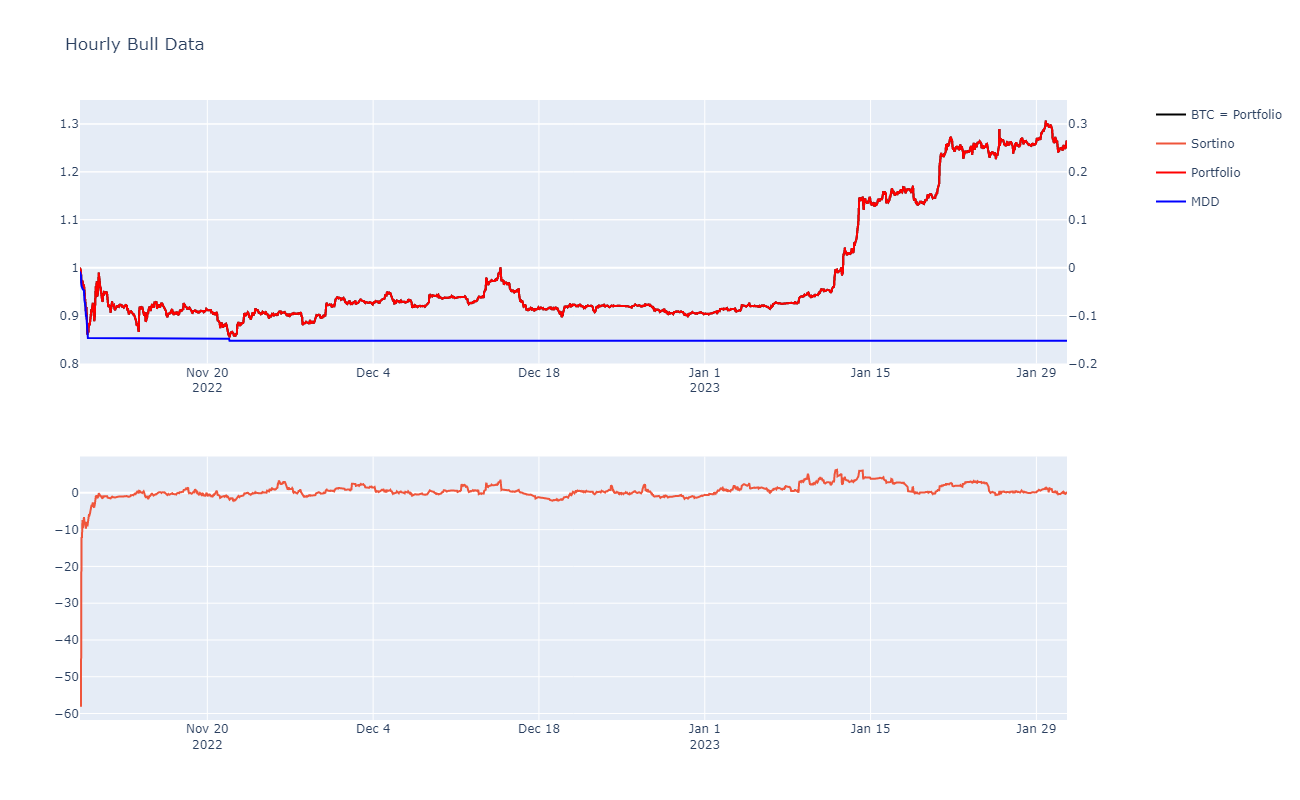
\includegraphics[width=0.94\textwidth]{graphics/results/01_hourly_bull.png}
    \caption{Buy-and-hold metrics for hourly bull data}
    \label{gr:bih:hbu}
\end{figure}

\begin{figure}[H]
    \centering
    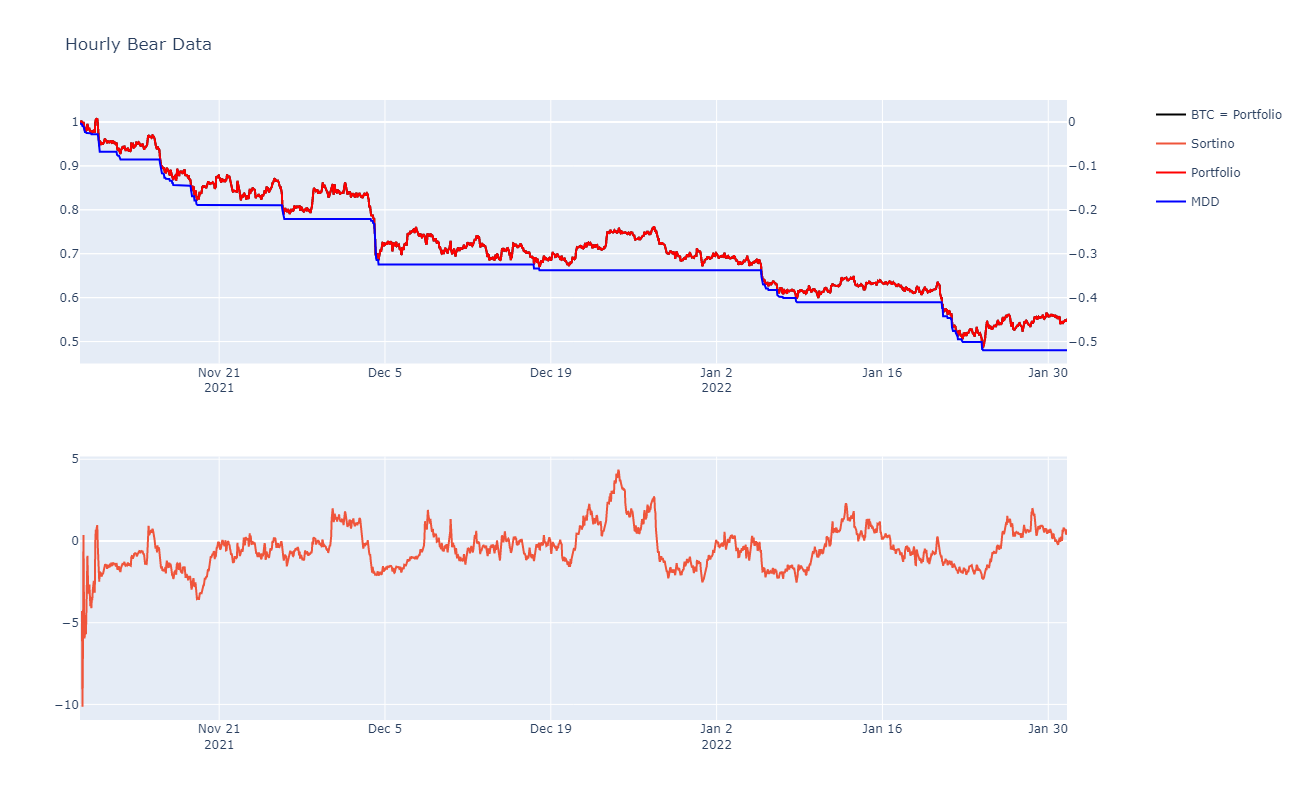
\includegraphics[width=0.94\textwidth]{graphics/results/01_hourly_bear.png}
    \caption{Buy-and-hold metrics for hourly bear data}
    \label{gr:bih:HBr}
\end{figure}

\begin{figure}[H]
    \centering
    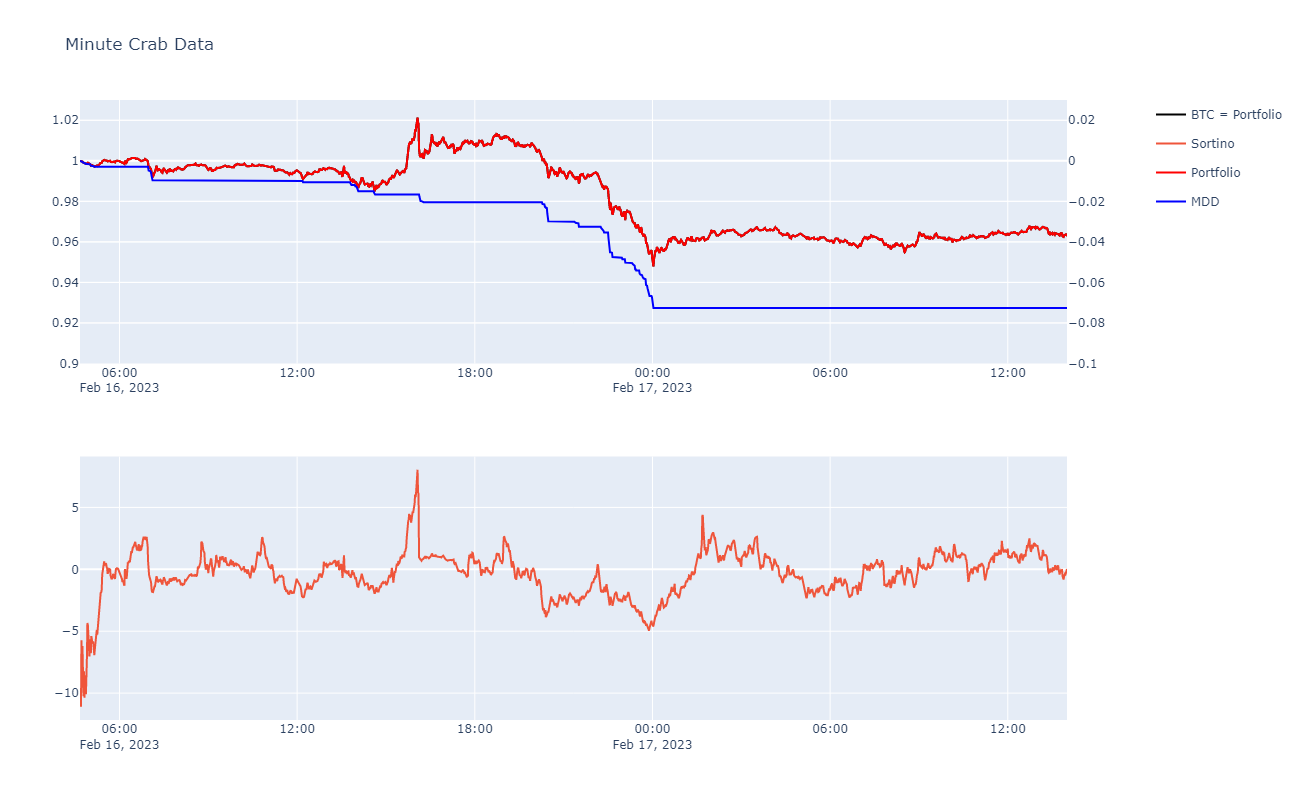
\includegraphics[width=0.94\textwidth]{graphics/results/01_minute_crab.png}
    \caption{Buy-and-hold metrics for minute crab data}
    \label{gr:bih:mcr}
\end{figure}

\begin{figure}[H]
    \centering
    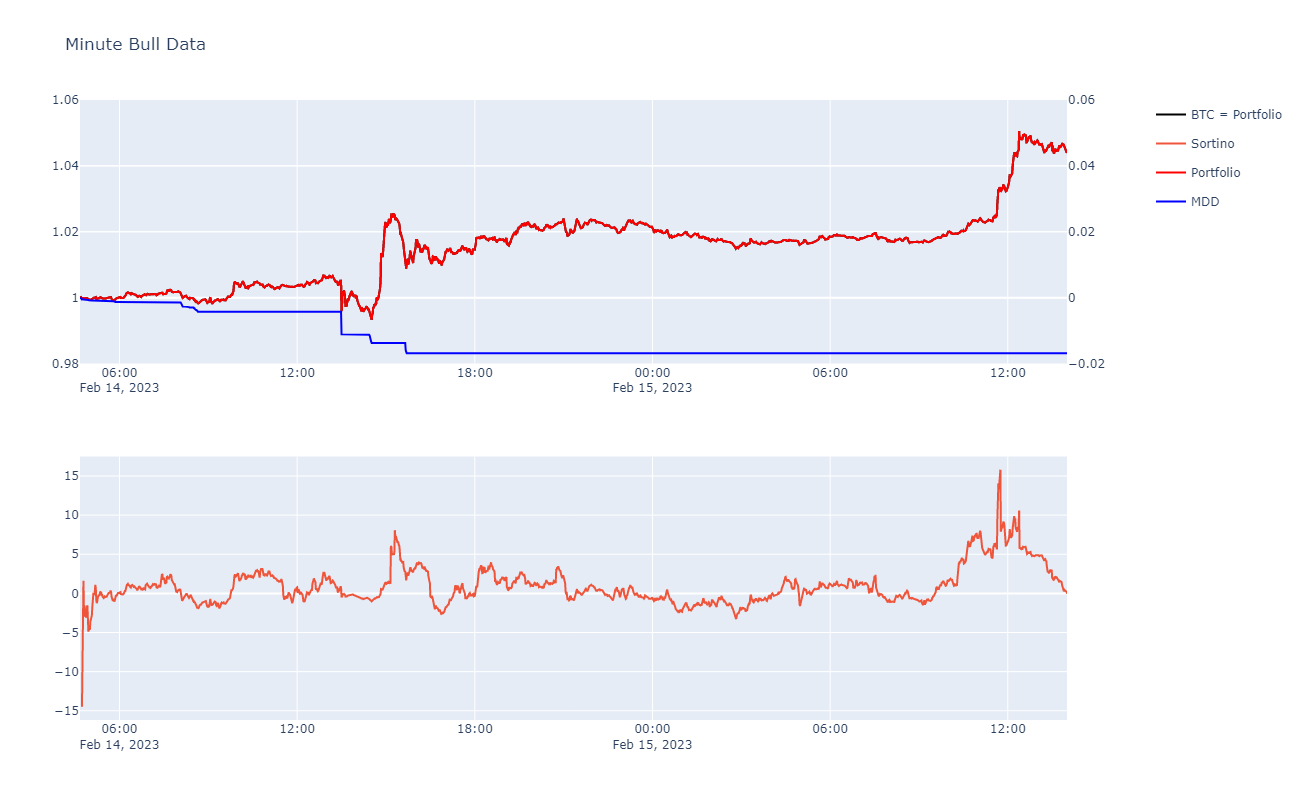
\includegraphics[width=0.94\textwidth]{graphics/results/01_minute_bull.png}
    \caption{Buy-and-hold metrics for minute bull data}
    \label{gr:bih:mbu}
\end{figure}

\subsection{MACD Strategy Agent}
The MACD strategy agent's performance statistics are shown in Table \ref{tab:res-macd}. Since this agent is not a learning agent, the values of $s$, $\tau$, and $\iota$ remain undefined.

Observe that this agent dampens the drawdown and loss in downtrend markets (figs. \ref{gr:macd:HBr}, \ref{gr:macd:mcr}), yet it also limits the profits for some cases and some periods in bull markets (figs. \ref{gr:macd:hbu}, \ref{gr:macd:mbu}). Moreover, MACD strategy shows that it can reduce MDD in all four cases. As for MACD strategy's Sortino ratio, it performs better than benchmark in bear markets, but never in bull or crab markets.

\begin{longtable}[c]{|l|r|r|r|c|c|c|l|}
\caption{MACD strategy agent statistics}
\label{tab:res-macd}\\
\hline
\multicolumn{1}{|c|}{} & \multicolumn{1}{c|}{\textbf{Return}} & \multicolumn{1}{c|}{\textbf{MDD}} & \multicolumn{1}{c|}{\textbf{Sortino}} &
\multicolumn{1}{c|}{\textbf{$\overline{\Delta\phi_{MACD,\odot}}$}} & \textbf{\textit{$s$}} & \multicolumn{1}{c|}{\textbf{Figure}} \\ \hline
\endfirsthead
%
\multicolumn{7}{c}%
{{\bfseries Table \thetable\ continued from previous page}} \\
\endhead
%
\textbf{\texttt{HBu}} & 0.2161 & 0.1159 & 0.0421 & 0.0620 & - &  \ref{gr:macd:hbu} \\ \hline
\textbf{\texttt{HBr}} & -0.3389 & 0.3570 & 0.6351 & 0.1363 & - &  \ref{gr:macd:HBr} \\ \hline
\textbf{\texttt{MCr}} & -0.0148 & 0.0427 & 0.4893 & 0.0118 & - &  \ref{gr:macd:mcr} \\ \hline
\textbf{\texttt{MBu}} & 0.0364 & 0.0124 & -0.1592 & -0.0008 & - &  \ref{gr:macd:mbu} \\ \hline
\end{longtable}

Figures \ref{gr:macd:HBr}, \ref{gr:macd:hbu}, \ref{gr:macd:mcr}, and \ref{gr:macd:mbu} show the full per-timeframe statistics of the recorded metrics. The upper part of the graphs shows three lines: (1) Black line: BTC closing price of each timeframe relative to the closing price of the first timeframe, (2) Red line: portfolio value of each timeframe relative to the initial investment, (3) Blue line: maximum drawdown of the portfolio. The lower part of the graphs contains two information: (1) Green line: 100-timeframe Sortino ratio of each timeframe, (2) Bar chart: shows the value of \texttt{macd\_histo} at each timeframe.

\begin{figure}[H]
    \centering
    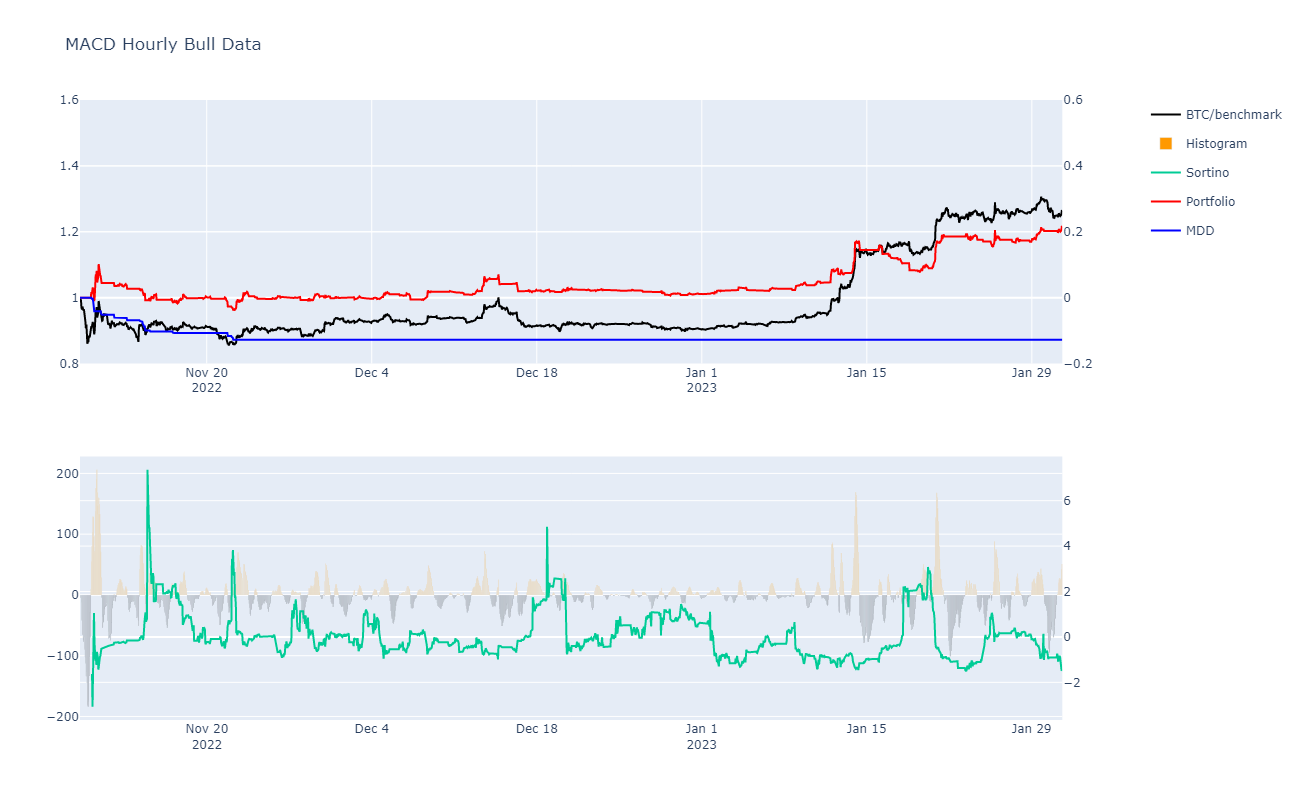
\includegraphics[width=0.94\textwidth]{graphics/results/02_macd_hourly_bull.png}
    \caption{MACD strategy metrics for hourly bull data}
    \label{gr:macd:hbu}
\end{figure}

\begin{figure}[H]
    \centering
    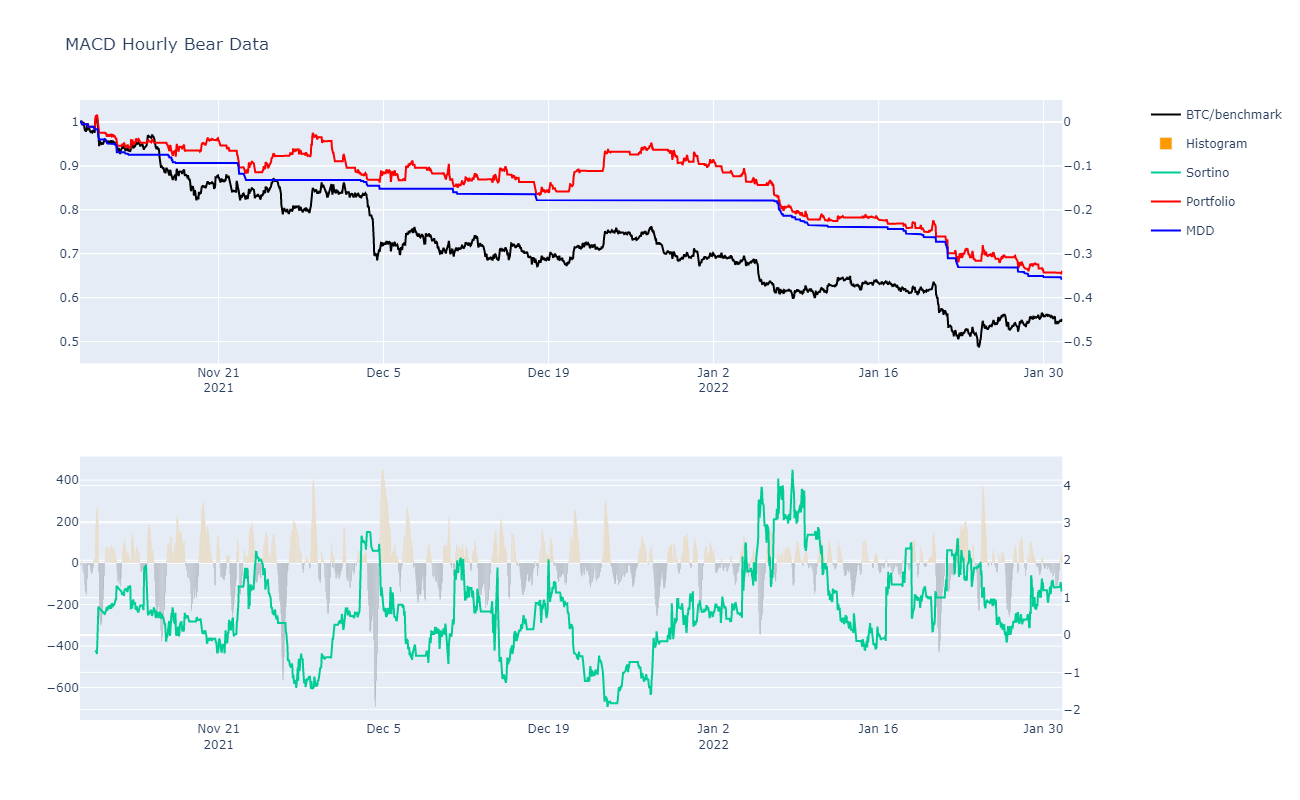
\includegraphics[width=0.94\textwidth]{graphics/results/02_macd_hourly_bear.png}
    \caption{MACD strategy metrics for hourly bear data}
    \label{gr:macd:HBr}
\end{figure}

\begin{figure}[H]
    \centering
    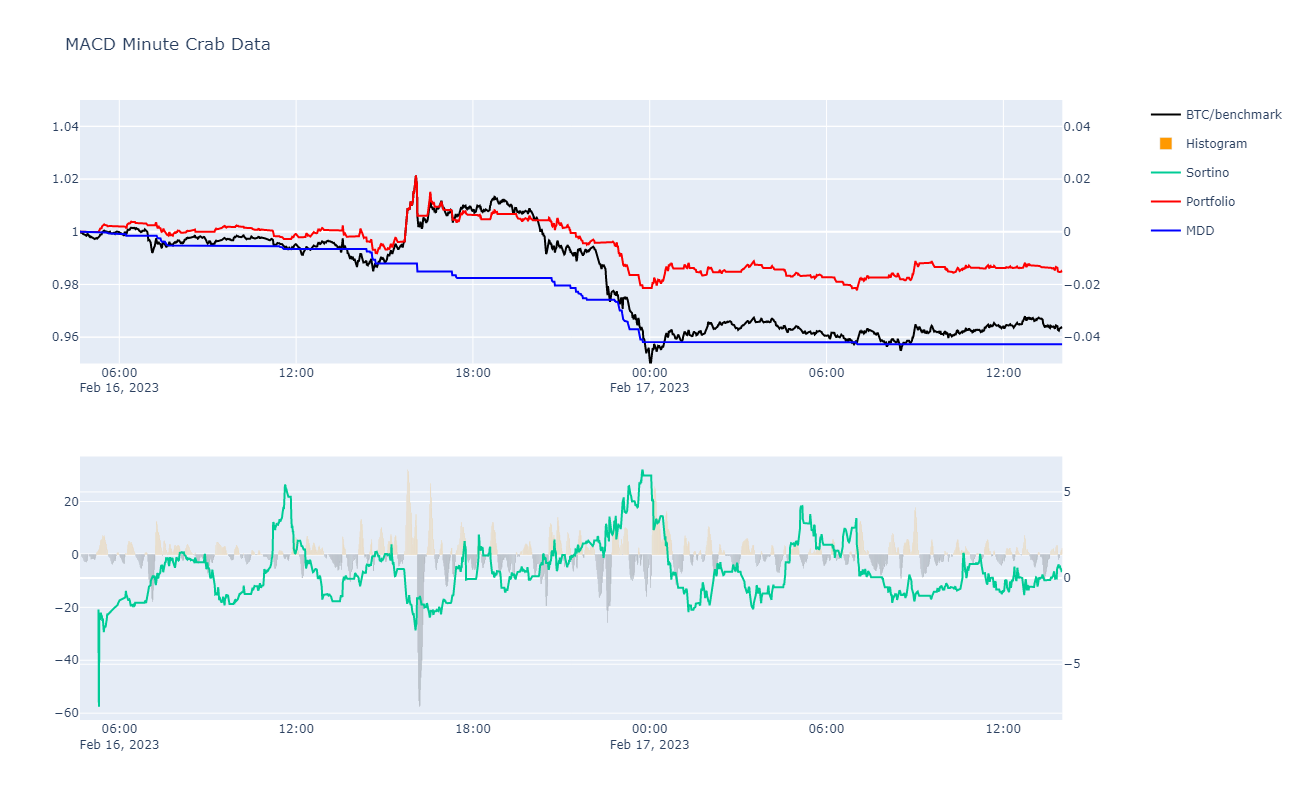
\includegraphics[width=0.94\textwidth]{graphics/results/02_macd_minute_crab.png}
    \caption{MACD strategy metrics for minute crab data}
    \label{gr:macd:mcr}
\end{figure}

\begin{figure}[H]
    \centering
    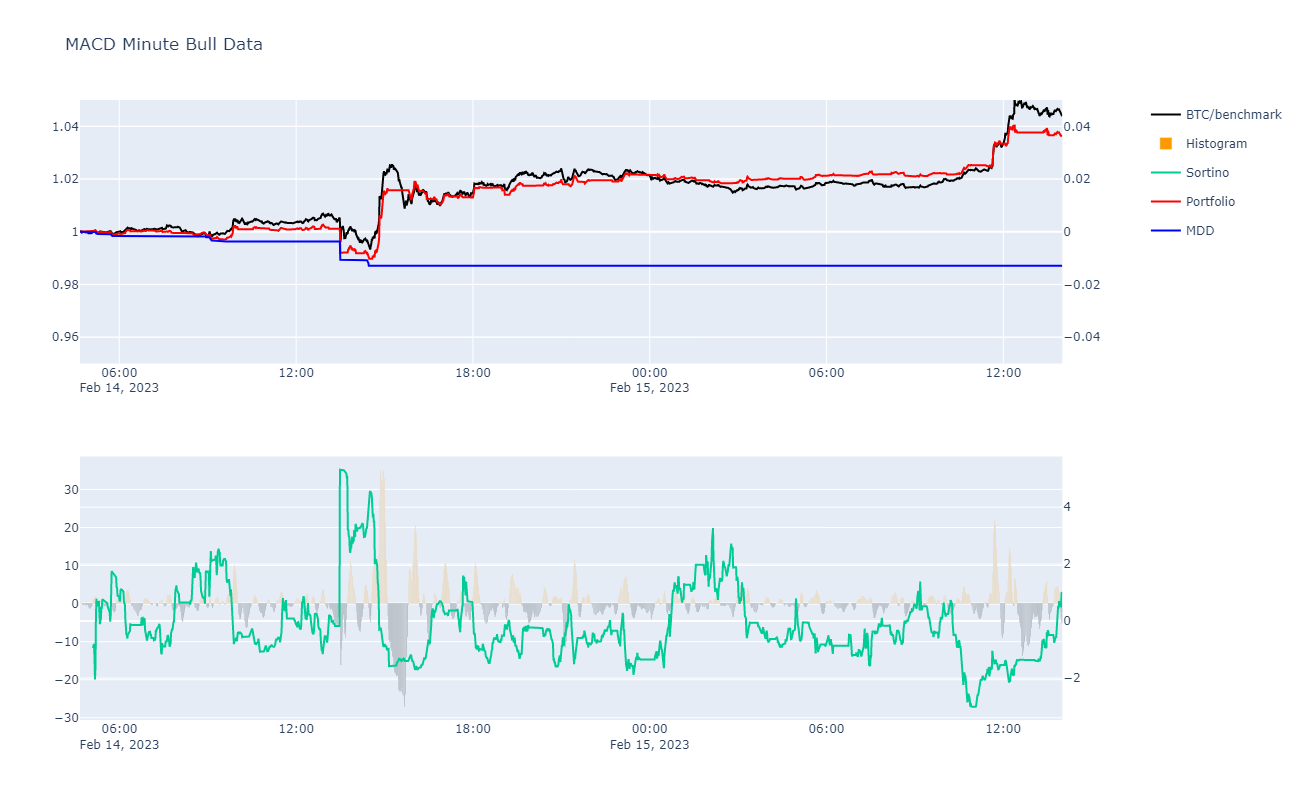
\includegraphics[width=0.94\textwidth]{graphics/results/02_macd_minute_bull.png}
    \caption{MACD strategy metrics for minute bull data}
    \label{gr:macd:mbu}
\end{figure}

\subsection{DQN Strategy Agent (Discrete)}
The DQN agent is the first RL agent to be presented in this chapter, operating in the discrete action space. Using training data (see Fig. \ref{gr:dqn:train}), the agent performs best only at early timestamps (between 100,000 to 500,000 timesteps $\approx$ 9 to 45 episodes). After around $s=$ 768,936 timestamps or 69 episodes ($\sim$2,500 seconds of training), the rewards and return value flatten.

\begin{figure}[H]
    \centering
    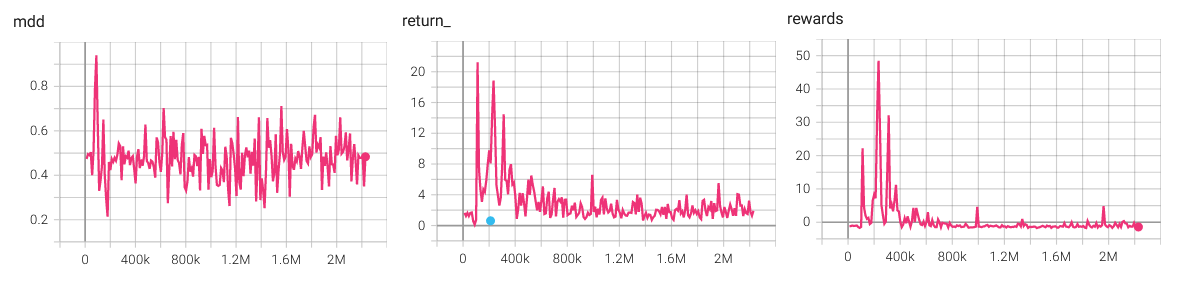
\includegraphics[width=0.99\textwidth]{graphics/trainphoto/dqntrain.png}
    \caption{DQN Training Results}
    \label{gr:dqn:train}
\end{figure}

DQN Agent's test results are given in Table \ref{resl:dqn}. By the average portfolio value over benchmark, the DQN agent outperforms the benchmark in all cases, while it fails to give the highest final value for \texttt{HBu} and \texttt{MBu} test datasets. The DQN agent, however, produces lower MDD which signifies that this agent is more risk-averse than the buy-and-hold agent.

\begin{longtable}[c]{|l|rrr|rrr|r|c|}
\caption{DQN Test Results}
\label{resl:cont-dqn}\\
\hline
\multicolumn{1}{|c|}{\multirow{2}{*}{\textbf{$\mathcal{D}$}}} & \multicolumn{3}{c|}{\textbf{Agent}} & \multicolumn{3}{c|}{\textbf{Benchmark}} & \multicolumn{1}{c|}{\multirow{2}{*}{\textbf{$\overline{\Delta\phi_{\alpha,\odot}}$}}} & \multirow{2}{*}{\textbf{Fig.}} \\ \cline{2-7}
\multicolumn{1}{|c|}{} & \multicolumn{1}{c|}{\textbf{Return}} & \multicolumn{1}{c|}{\textbf{MDD}} & \multicolumn{1}{c|}{\textit{\textbf{Sortino}}} & \multicolumn{1}{c|}{\textbf{Return}} & \multicolumn{1}{c|}{\textbf{MDD}} & \multicolumn{1}{c|}{\textit{\textbf{Sortino}}} & \multicolumn{1}{c|}{} &  \\ \hline
\endfirsthead
%
\multicolumn{9}{c}%
{{\bfseries Table \thetable\ continued from previous page}} \\
\endhead
%
\textbf{\texttt{HBu}} & \multicolumn{1}{r|}{0.1540} & \multicolumn{1}{r|}{0.1812} & \textit{-0.2212} & \multicolumn{1}{r|}{\textbf{0.2643}} & \multicolumn{1}{r|}{\textbf{0.1174}} & \textit{0.7060} & 0.0204 & \ref{f-dqn-hbu} \\ \hline
\textbf{\texttt{HBr}} & \multicolumn{1}{r|}{\textbf{-0.1184}} & \multicolumn{1}{r|}{\textbf{0.1343}} & \textit{0.7485} & \multicolumn{1}{r|}{-0.4484} & \multicolumn{1}{r|}{0.5199} & \textit{-0.3982} & 0.3015 & \ref{f-dqn-hbr} \\ \hline
\textbf{\texttt{MCr}} & \multicolumn{1}{r|}{\textbf{0.0296}} & \multicolumn{1}{r|}{\textbf{0.0313}} & \textit{1.1557} & \multicolumn{1}{r|}{-0.0361} & \multicolumn{1}{r|}{0.0725} & \textit{-0.2276} & 0.0383 & \ref{f-dqn-mcr} \\ \hline
\textbf{\texttt{MBu}} & \multicolumn{1}{r|}{0.0357} & \multicolumn{1}{r|}{\textbf{0.0061}} & \textit{-0.3521} & \multicolumn{1}{r|}{\textbf{0.0441}} & \multicolumn{1}{r|}{0.0164} & \textit{1.0024} & 0.0102 & \ref{f-dqn-mbu} \\ \hline
\end{longtable}

\begin{figure}[H]
    \centering
    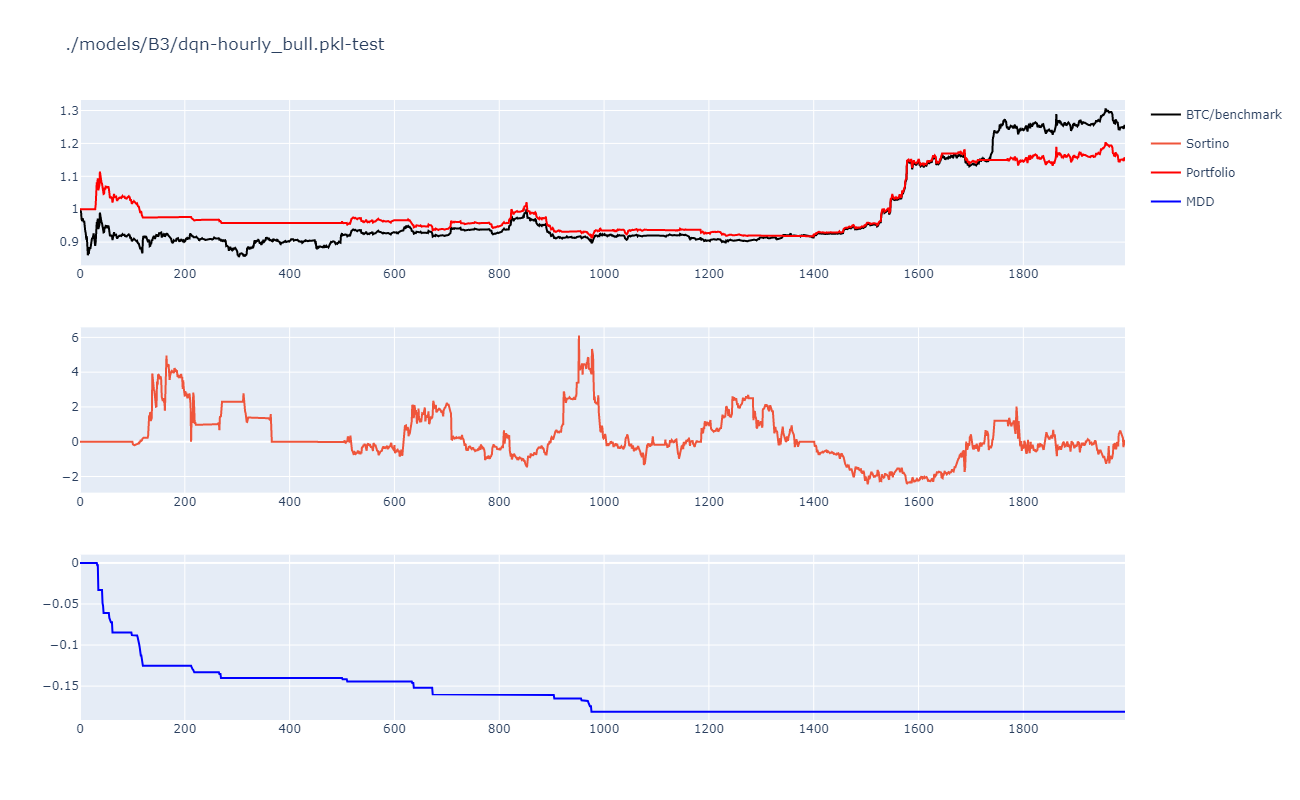
\includegraphics[width=0.94\textwidth]{graphics/testphoto/dqn-hbu.png}
    \caption{DQN agent metrics for hourly bull data}
    \label{f-dqn-hbu}
\end{figure}

\begin{figure}[H]
    \centering
    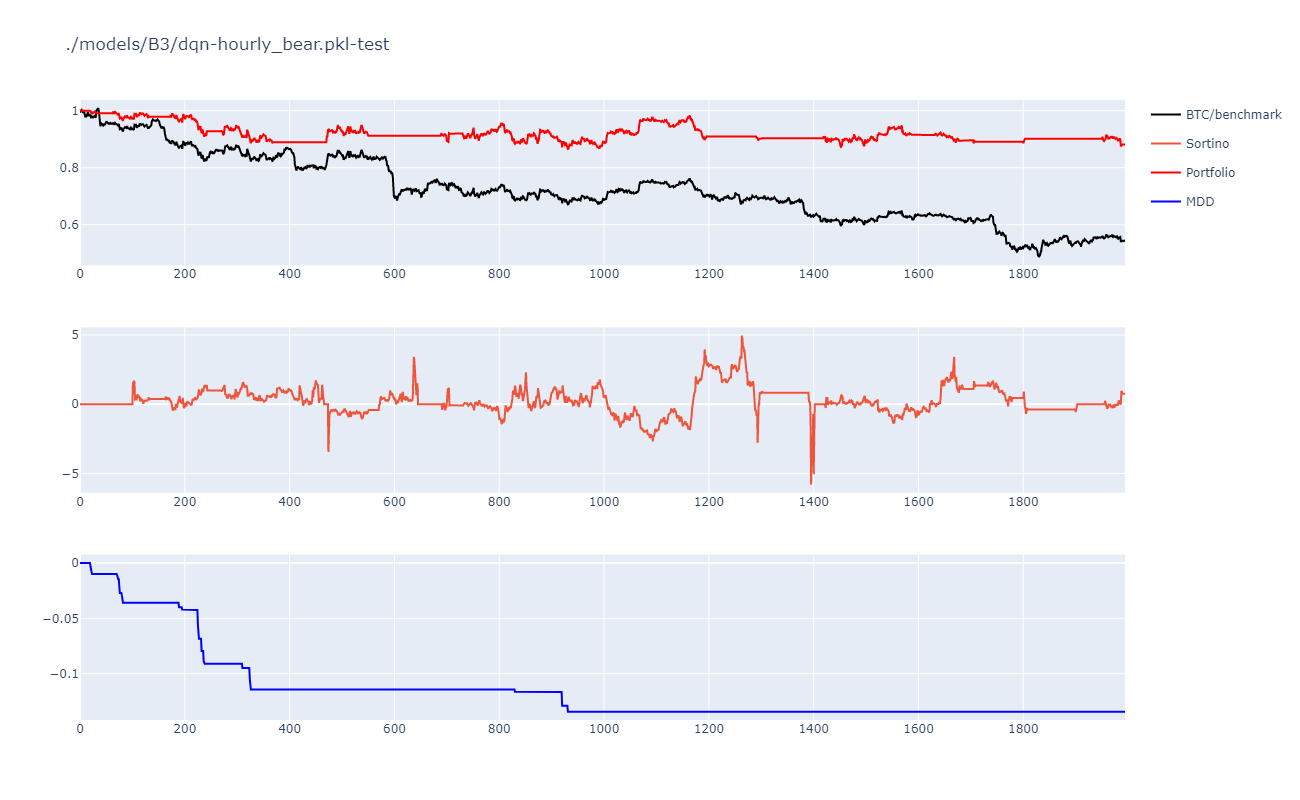
\includegraphics[width=0.94\textwidth]{graphics/testphoto/dqn-hbr.png}
    \caption{DQN agent metrics for hourly bear data}
    \label{f-dqn-hbr}
\end{figure}

\begin{figure}[H]
    \centering
    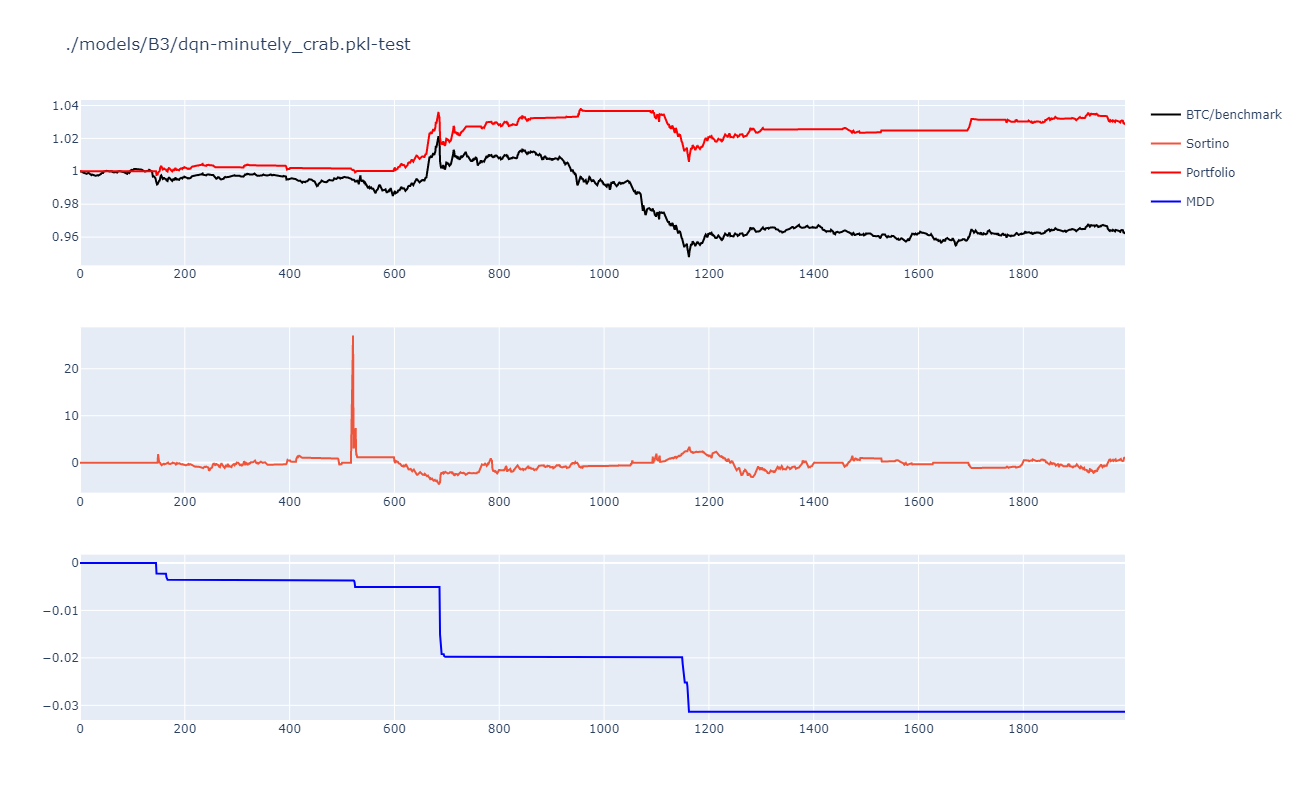
\includegraphics[width=0.94\textwidth]{graphics/testphoto/dqn-mcr.png}
    \caption{DQN agent metrics for minute crab data}
    \label{f-dqn-mcr}
\end{figure}

\begin{figure}[H]
    \centering
    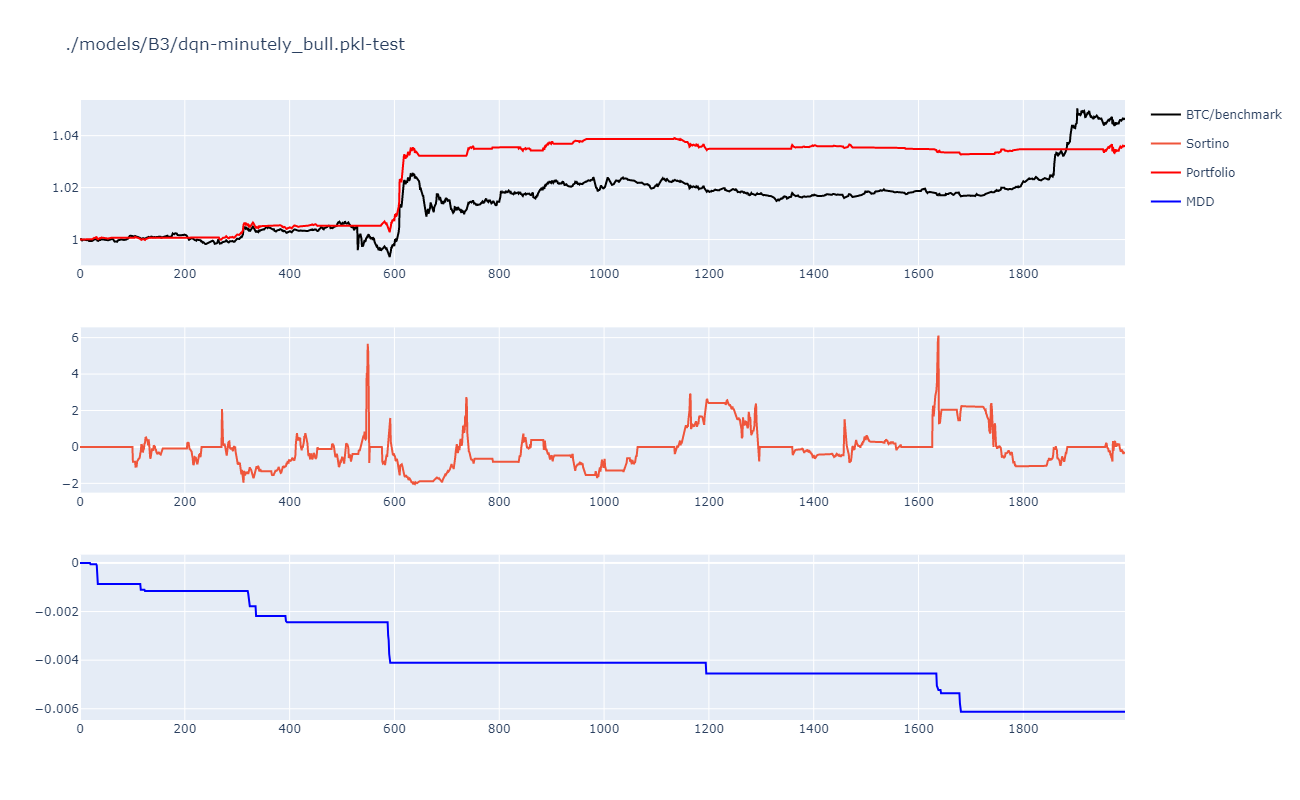
\includegraphics[width=0.94\textwidth]{graphics/testphoto/dqn-mbu.png}
    \caption{DQN agent metrics for minute bull data}
    \label{f-dqn-mbu}
\end{figure}

\subsection{A2C Strategy Agent (Discrete)}
This A2C agent is used with a discrete action space. Using training data (see Fig. \ref{gr:a2cd:train}), the agent, by all factors, converges quickly at around $\sim$45,000 timesteps (4 episodes, $\sim$90 seconds of training). After that, there is virtually no improvement nor deterioration of the model.

\begin{figure}[H]
    \centering
    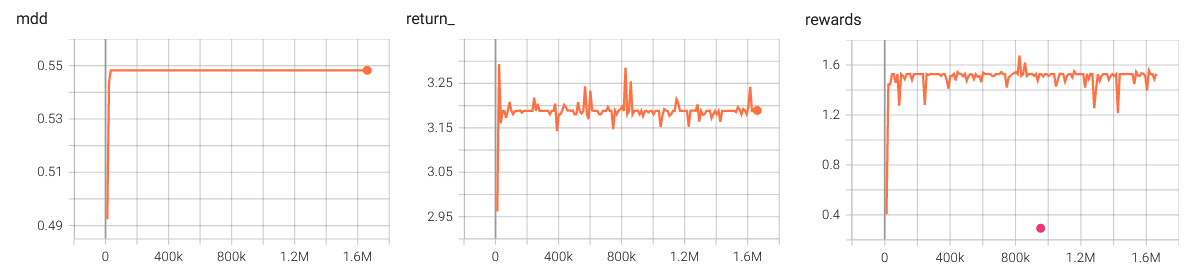
\includegraphics[width=0.99\textwidth]{graphics/trainphoto/a2cd-train.png}
    \caption{Discrete A2C Training Results}
    \label{gr:a2cd:train}
\end{figure}

Despite the quick stable model turnout, it is suspected that the model only performs a minimal number of trades and just holds the one-time bought until the end, rendering it to be exactly comparable with the buy-and-hold agent. Refer to Table \ref{resl:disc-a2c}'s $\overline{\Delta\phi_{\alpha,\odot}}$ column which shows that the average difference between the portfolio values of this agent and the benchmark agent is less than 0.5 percent in all cases.

\begin{longtable}[c]{|l|rrr|rrr|r|c|}
\caption{Discrete A2C Test Results}
\label{resl:disc-a2c}\\
\hline
\multicolumn{1}{|c|}{\multirow{2}{*}{\textbf{$\mathcal{D}$}}} & \multicolumn{3}{c|}{\textbf{Agent}} & \multicolumn{3}{c|}{\textbf{Benchmark}} & \multicolumn{1}{c|}{\multirow{2}{*}{\textbf{$\overline{\Delta\phi_{\alpha,\odot}}$}}} & \multirow{2}{*}{\textbf{Fig.}} \\ \cline{2-7}
\multicolumn{1}{|c|}{} & \multicolumn{1}{c|}{\textbf{Return}} & \multicolumn{1}{c|}{\textbf{MDD}} & \multicolumn{1}{c|}{\textit{\textbf{Sortino}}} & \multicolumn{1}{c|}{\textbf{Return}} & \multicolumn{1}{c|}{\textbf{MDD}} & \multicolumn{1}{c|}{\textit{\textbf{Sortino}}} & \multicolumn{1}{c|}{} &  \\ \hline
\endfirsthead
%
\multicolumn{9}{c}%
{{\bfseries Table \thetable\ continued from previous page}} \\
\endhead
%
\textbf{\texttt{HBu}} & \multicolumn{1}{r|}{0.2568} & \multicolumn{1}{r|}{0.1425} & \textit{-0.2843} & \multicolumn{1}{r|}{\textbf{0.2643}} & \multicolumn{1}{r|}{\textbf{0.1174}} & \textit{0.7060} & 0.0035 & \ref{f-a2c-cont-hbu} \\ \hline
\textbf{\texttt{HBr}} & \multicolumn{1}{r|}{-0.4543} & \multicolumn{1}{r|}{\textbf{0.5174}} & \textit{-0.7186} & \multicolumn{1}{r|}{\textbf{-0.4484}} & \multicolumn{1}{r|}{0.5199} & \textit{-0.3982} & -0.0009 & \ref{f-a2c-cont-hbr} \\ \hline
\textbf{\texttt{MCr}} & \multicolumn{1}{r|}{-0.0368} & \multicolumn{1}{r|}{\textbf{0.0719}} & \textit{0.8994} & \multicolumn{1}{r|}{\textbf{-0.0361}} & \multicolumn{1}{r|}{0.0725} & \textit{-0.2276} & 0.0000 & \ref{f-a2c-cont-mcr} \\ \hline
\textbf{\texttt{MBu}} & \multicolumn{1}{r|}{\textbf{0.0462}} & \multicolumn{1}{r|}{0.0165} & \textit{-0.3752} & \multicolumn{1}{r|}{0.0441} & \multicolumn{1}{r|}{\textbf{0.0164}} & \textit{1.0024} & 0.0000 & \ref{f-a2c-cont-mbu} \\ \hline
\end{longtable}

\begin{figure}[H]
    \centering
    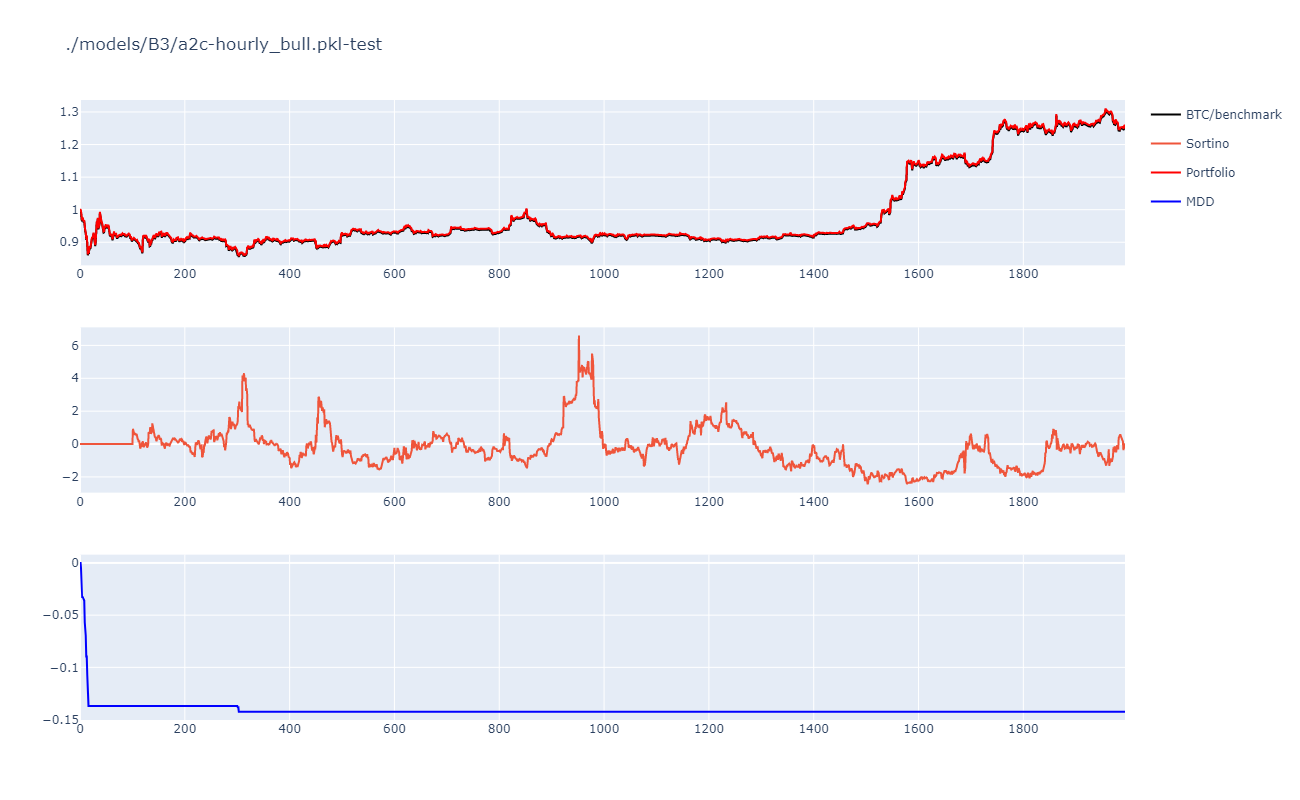
\includegraphics[width=0.94\textwidth]{graphics/testphoto/a2c-disc-hbu.png}
    \caption{Discrete A2C agent metrics for hourly bull data}
    \label{f-a2c-disc-hbu}
\end{figure}

\begin{figure}[H]
    \centering
    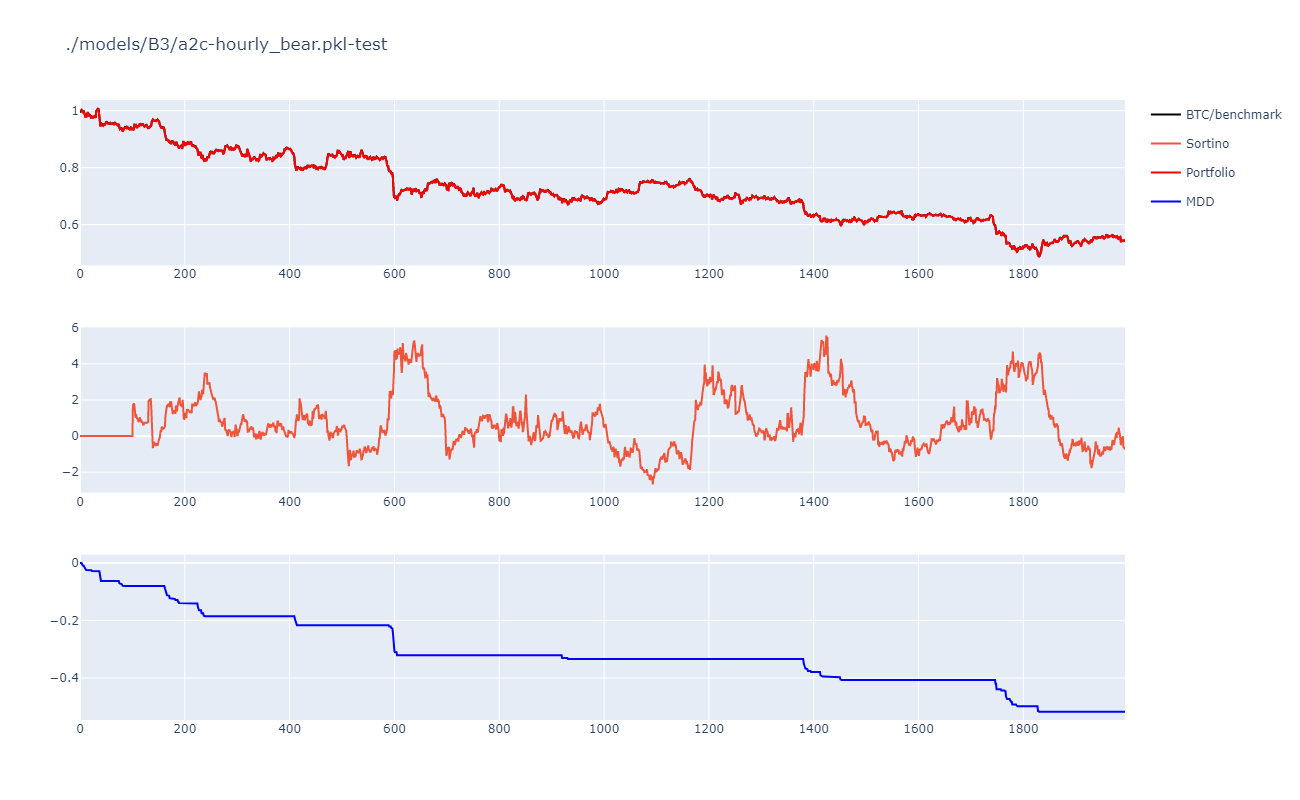
\includegraphics[width=0.94\textwidth]{graphics/testphoto/a2c-disc-hbr.png}
    \caption{Discrete A2C agent metrics for hourly bear data}
    \label{f-a2c-disc-hbr}
\end{figure}

\begin{figure}[H]
    \centering
    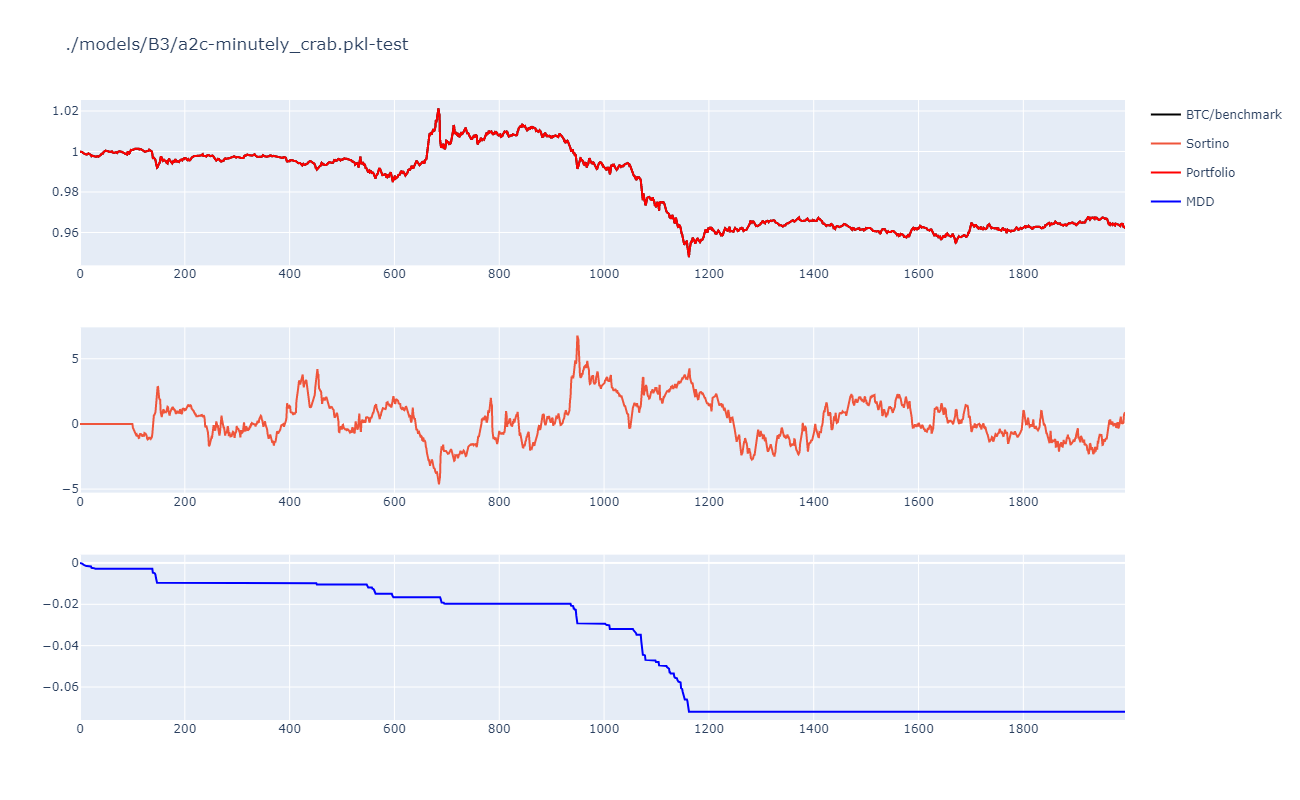
\includegraphics[width=0.94\textwidth]{graphics/testphoto/a2c-disc-mcr.png}
    \caption{Discrete A2C agent metrics for minute crab data}
    \label{f-a2c-disc-mcr}
\end{figure}

\begin{figure}[H]
    \centering
    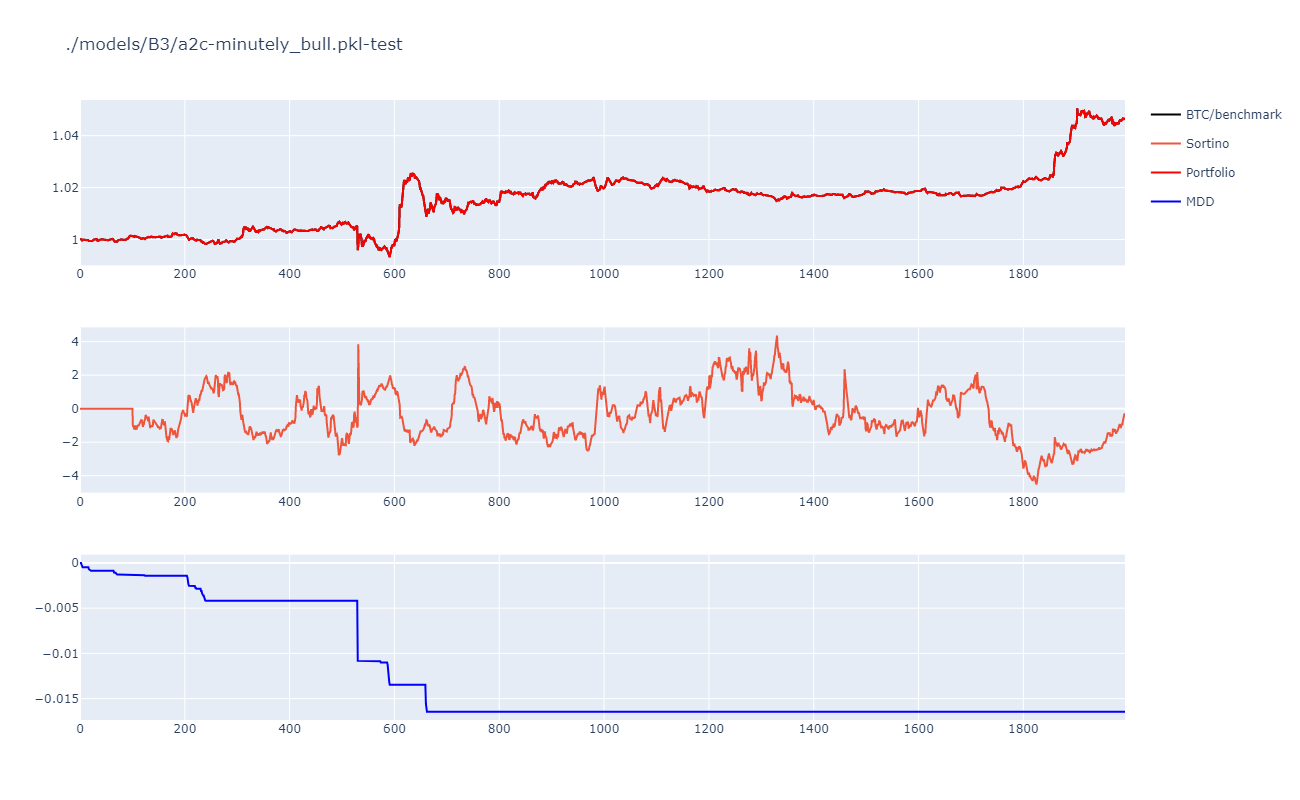
\includegraphics[width=0.94\textwidth]{graphics/testphoto/a2c-disc-mbu.png}
    \caption{Discrete A2C agent metrics for minute bull data}
    \label{f-a2c-disc-mbu}
\end{figure}

\subsection{A2C Strategy Agent (Continuous)}
This A2C agent is used with a continuous action space. Using training data (see Fig. \ref{gr:a2cd:train}), the agent never finds a stable ground even after more than 1,671,600 timestamps (150 episodes, 5,500 seconds): the total reward and return still fluctuates randomly, unlike its discrete counterpart. The models with zero reward did not generate any trade, including the final model, hence the last non-zero-reward model at timestamp 1,348,424 (121st episode) is taken as its representative model.

\begin{figure}[H]
    \centering
    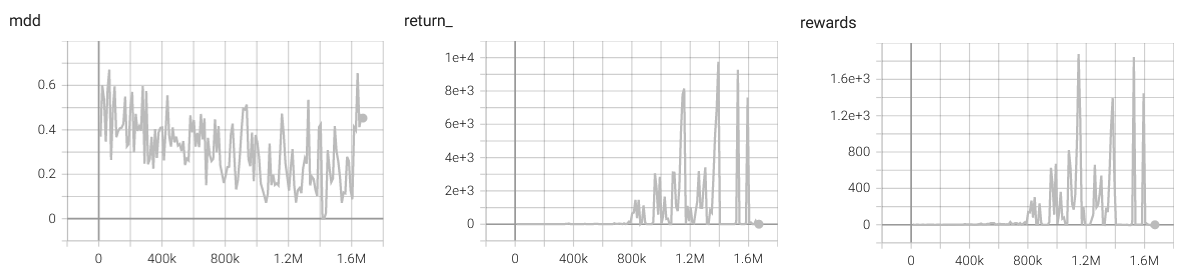
\includegraphics[width=0.99\textwidth]{graphics/trainphoto/a2cc-train.png}
    \caption{Continuous A2C Training Results}
    \label{gr:a2cc:train}
\end{figure}

Compared to the benchmark, the representative Continuous A2C model results in a slightly more satisfiable performance in minute test datasets, at 1.68\% (crab) and 0.23\% (bull) average portfolio differences, 40\% less drawdown, and higher final return. Conversely, this model fails to produce better performance than benchmark in all aspects. See Table \ref{resl:cont-a2c}.

\begin{longtable}[c]{|l|rrr|rrr|r|c|}
\caption{Continuous A2C Test Results}
\label{resl:cont-a2c}\\
\hline
\multicolumn{1}{|c|}{\multirow{2}{*}{\textbf{$\mathcal{D}$}}} & \multicolumn{3}{c|}{\textbf{Agent}} & \multicolumn{3}{c|}{\textbf{Benchmark}} & \multicolumn{1}{c|}{\multirow{2}{*}{\textbf{$\overline{\Delta\phi_{\alpha,\odot}}$}}} & \multirow{2}{*}{\textbf{Fig.}} \\ \cline{2-7}
\multicolumn{1}{|c|}{} & \multicolumn{1}{c|}{\textbf{Return}} & \multicolumn{1}{c|}{\textbf{MDD}} & \multicolumn{1}{c|}{\textit{\textbf{Sortino}}} & \multicolumn{1}{c|}{\textbf{Return}} & \multicolumn{1}{c|}{\textbf{MDD}} & \multicolumn{1}{c|}{\textit{\textbf{Sortino}}} & \multicolumn{1}{c|}{} &  \\ \hline
\endfirsthead
%
\multicolumn{9}{c}%
{{\bfseries Table \thetable\ continued from previous page}} \\
\endhead
%
\textbf{\texttt{HBu}} & \multicolumn{1}{r|}{0.0060} & \multicolumn{1}{r|}{0.1622} & \textit{-0.5541} & \multicolumn{1}{r|}{\textbf{0.2643}} & \multicolumn{1}{r|}{\textbf{0.1174}} & \textit{0.7060} & -0.0602 & \ref{f-a2c-disc-hbu} \\ \hline
\textbf{\texttt{HBr}} & \multicolumn{1}{r|}{-0.4824} & \multicolumn{1}{r|}{0.5618} & \textit{-1.6495} & \multicolumn{1}{r|}{\textbf{-0.4484}} & \multicolumn{1}{r|}{\textbf{0.5199}} & \textit{-0.3982} & -0.0320 & \ref{f-a2c-disc-hbr} \\ \hline
\textbf{\texttt{MCr}} & \multicolumn{1}{r|}{\textbf{-0.0137}} & \multicolumn{1}{r|}{\textbf{0.0462}} & \textit{0.6625} & \multicolumn{1}{r|}{-0.0361} & \multicolumn{1}{r|}{0.0725} & \textit{-0.2276} & 0.0168 & \ref{f-a2c-disc-mcr} \\ \hline
\textbf{\texttt{MBu}} & \multicolumn{1}{r|}{\textbf{0.0480}} & \multicolumn{1}{r|}{\textbf{0.0101}} & \textit{-1.2651} & \multicolumn{1}{r|}{0.0441} & \multicolumn{1}{r|}{0.0164} & \textit{1.0024} & 0.0023 & \ref{f-a2c-disc-mbu} \\ \hline
\end{longtable}

\begin{figure}[H]
    \centering
    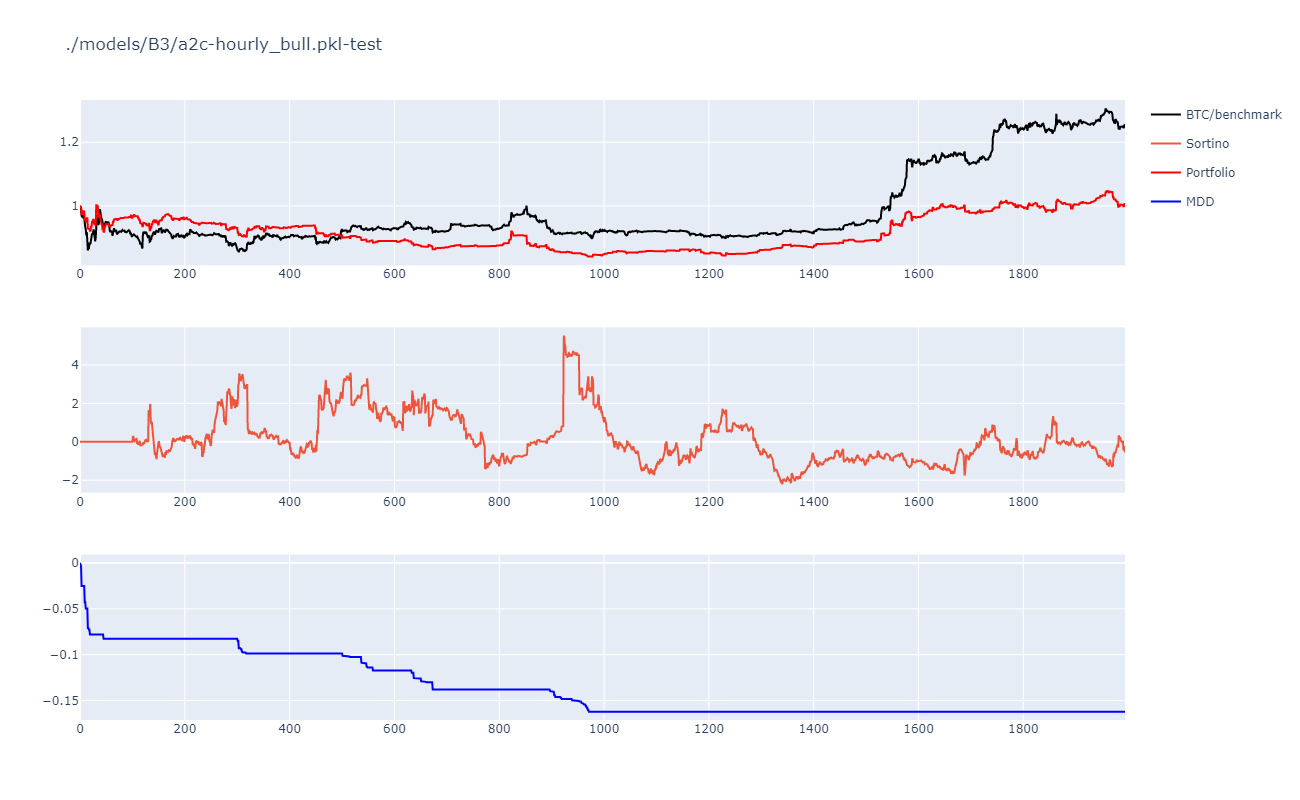
\includegraphics[width=0.94\textwidth]{graphics/testphoto/a2c-cont-hbu.png}
    \caption{Continuous A2C agent metrics for hourly bull data}
    \label{f-a2c-cont-hbu}
\end{figure}

\begin{figure}[H]
    \centering
    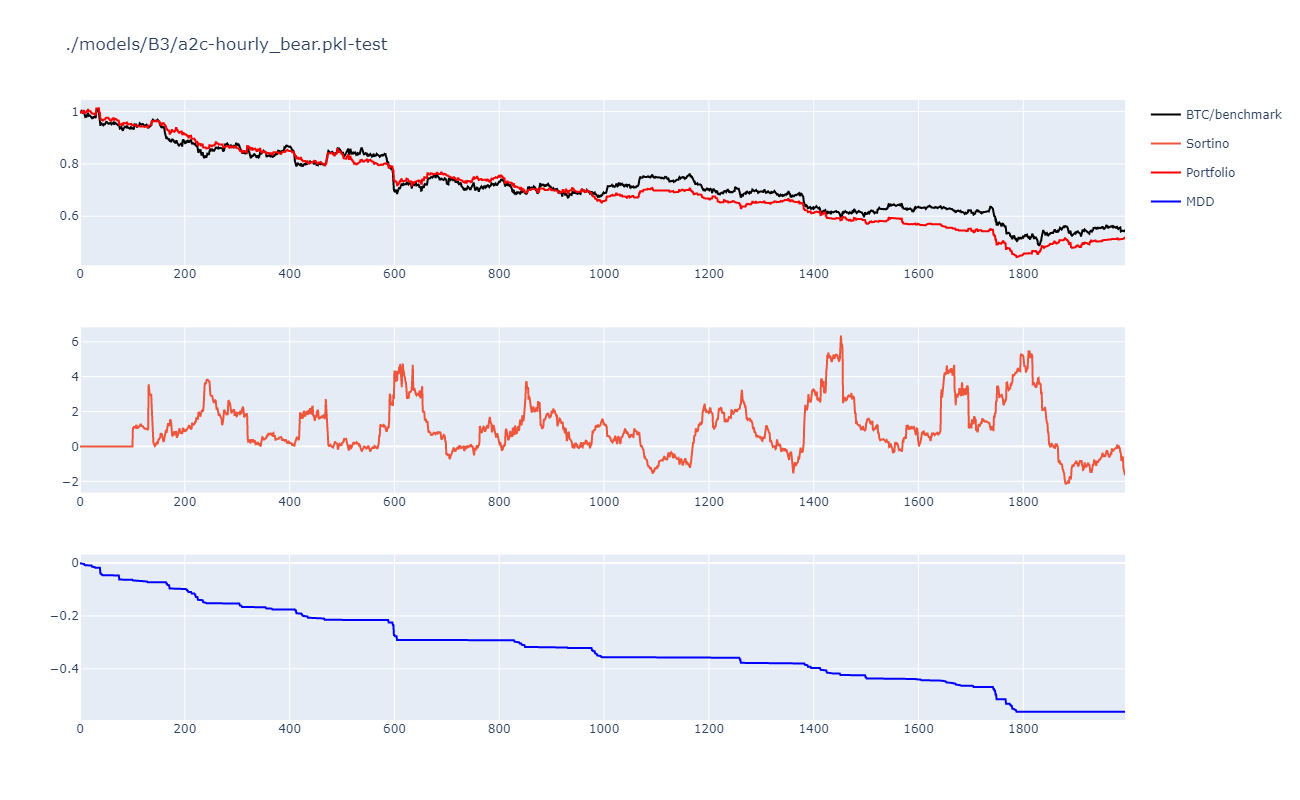
\includegraphics[width=0.94\textwidth]{graphics/testphoto/a2c-cont-hbr.png}
    \caption{Continuous A2C agent metrics for hourly bear data}
    \label{f-a2c-cont-hbr}
\end{figure}

\begin{figure}[H]
    \centering
    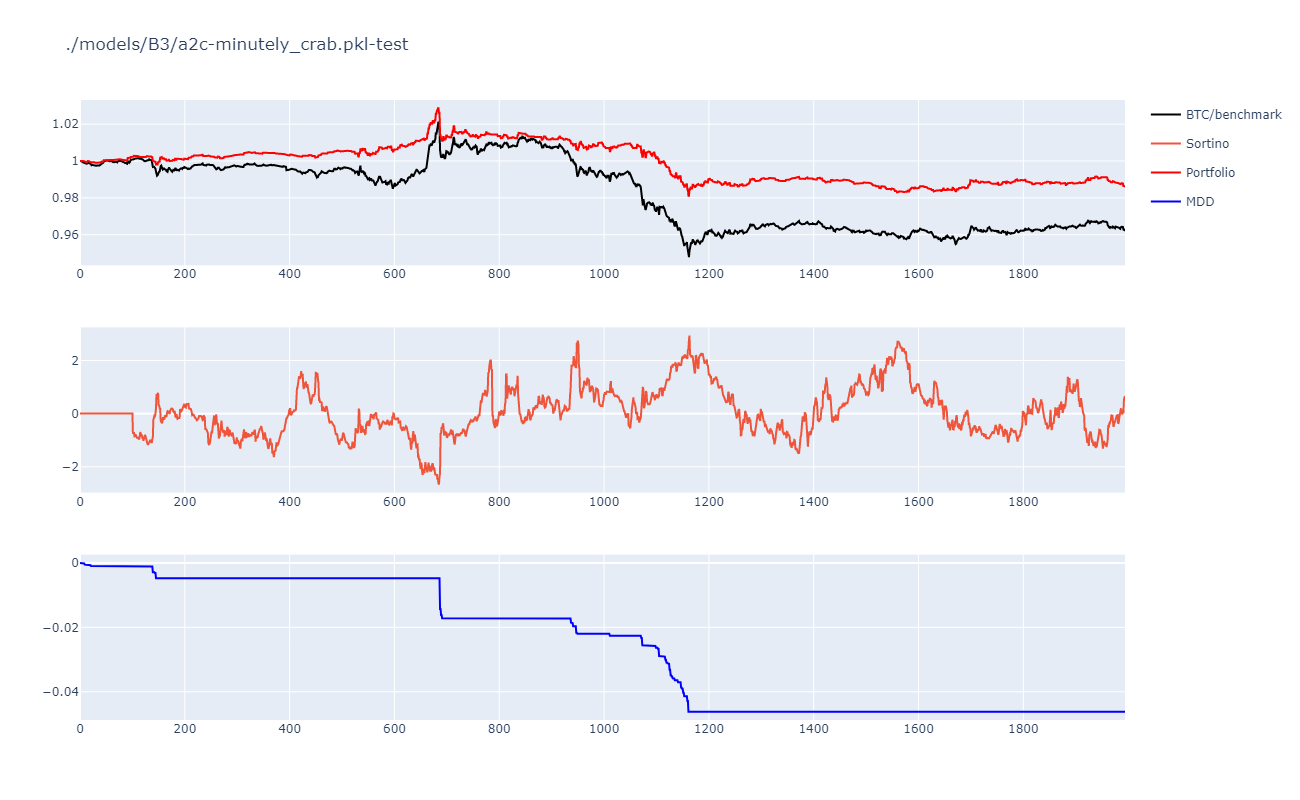
\includegraphics[width=0.94\textwidth]{graphics/testphoto/a2c-cont-mcr.png}
    \caption{Continuous A2C agent metrics for minute crab data}
    \label{f-a2c-cont-mcr}
\end{figure}

\begin{figure}[H]
    \centering
    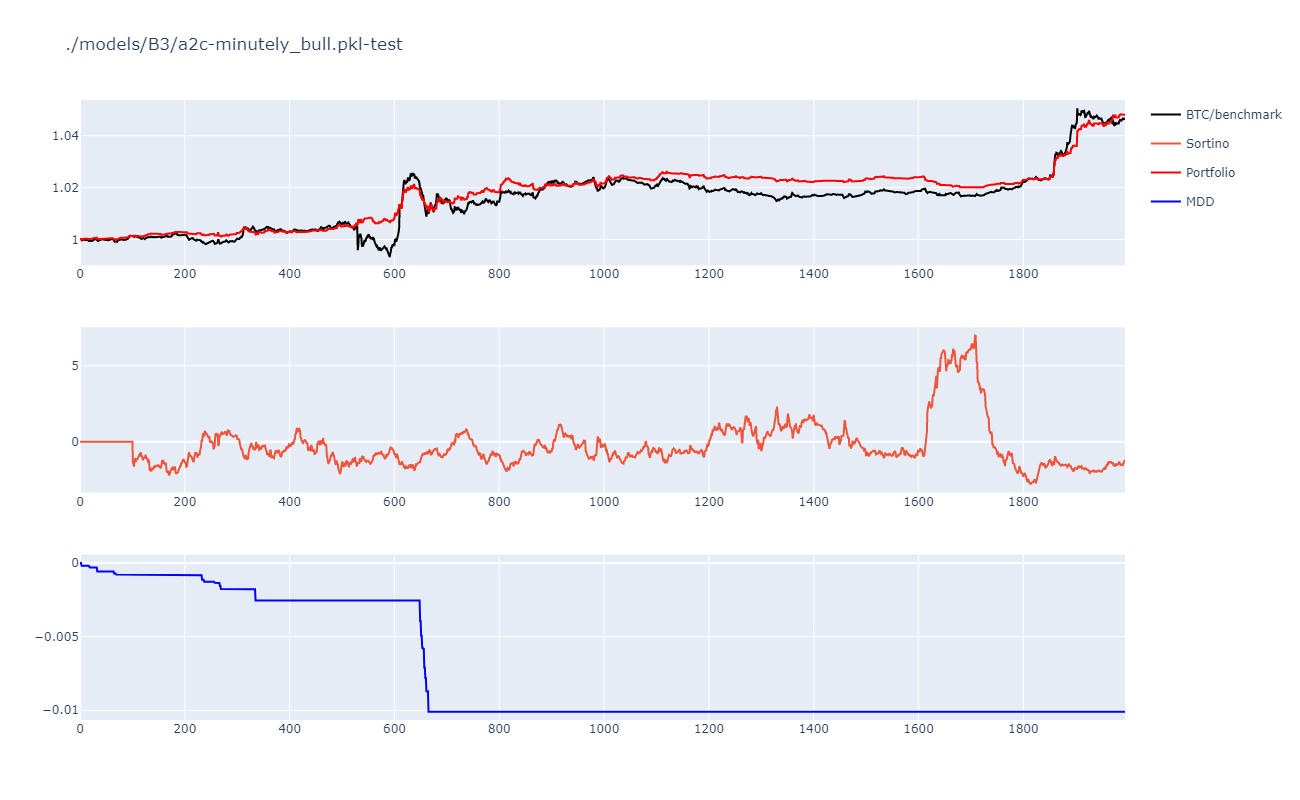
\includegraphics[width=0.94\textwidth]{graphics/testphoto/a2c-cont-mbu.png}
    \caption{Continuous A2C agent metrics for minute bull data}
    \label{f-a2c-cont-mbu}
\end{figure}

\subsection{PPO Strategy Agent (Discrete)}
This PPO agent is used with a discrete action space. The Discrete PPO agent performed weakly at the first 2 million timestamps, then surged after. Among 10 training runs, similar peaks appear and vanish in a similar way at random episodes. The representative model is taken from the final result of the training session shown in Fig. \ref{gr:ppod:train}, at timestamp 2,228,800 (200th episode, $\sim$5,000 seconds).

\begin{figure}[H]
    \centering
    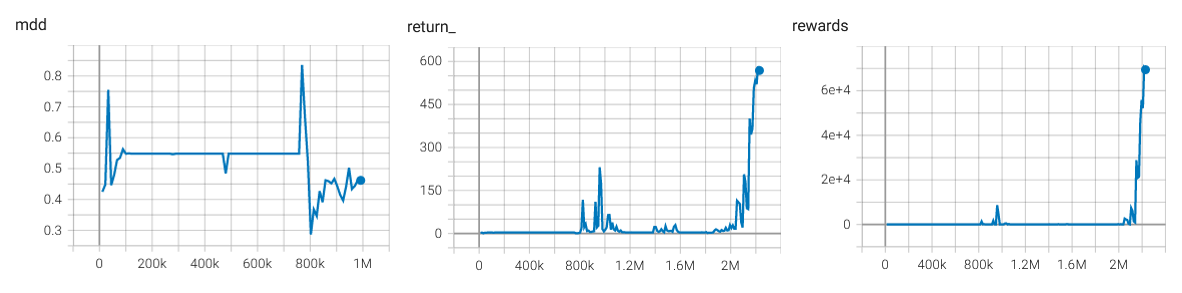
\includegraphics[width=0.99\textwidth]{graphics/trainphoto/ppodtrain.png}
    \caption{Discrete PPO Training Results}
    \label{gr:ppod:train}
\end{figure}

The model, scoring 600 at training return value, i.e., 59,900\% profit over the training data, results in a significant profit in \texttt{HBu} and \texttt{HBr} test datasets, performing in average 59.88\% and 153.96\% better than benchmark, respectively. However, the Discrete PPO agent is not much better than benchmark in minute test datasets. Overall, it performs better in all aspects (return, MDD) compared to the benchmark. See Table \ref{resl:disc-ppo}.

\begin{longtable}[c]{|l|rrr|rrr|r|c|}
\caption{Discrete PPO Test Results}
\label{resl:disc-ppo}\\
\hline
\multicolumn{1}{|c|}{\multirow{2}{*}{\textbf{$\mathcal{D}$}}} & \multicolumn{3}{c|}{\textbf{Agent}} & \multicolumn{3}{c|}{\textbf{Benchmark}} & \multicolumn{1}{c|}{\multirow{2}{*}{\textbf{$\overline{\Delta\phi_{\alpha,\odot}}$}}} & \multirow{2}{*}{\textbf{Fig.}} \\ \cline{2-7}
\multicolumn{1}{|c|}{} & \multicolumn{1}{c|}{\textbf{Return}} & \multicolumn{1}{c|}{\textbf{MDD}} & \multicolumn{1}{c|}{\textit{\textbf{Sortino}}} & \multicolumn{1}{c|}{\textbf{Return}} & \multicolumn{1}{c|}{\textbf{MDD}} & \multicolumn{1}{c|}{\textit{\textbf{Sortino}}} & \multicolumn{1}{c|}{} &  \\ \hline
\endfirsthead
%
\multicolumn{9}{c}%
{{\bfseries Table \thetable\ continued from previous page}} \\
\endhead
%
\textbf{\texttt{HBu}} & \multicolumn{1}{r|}{\textbf{1.6982}} & \multicolumn{1}{r|}{\textbf{0.0725}} & \textit{-1.1362} & \multicolumn{1}{r|}{0.2643} & \multicolumn{1}{r|}{0.1174} & \textit{0.7060} & 0.5988 & \ref{f-ppo-disc-hbu} \\ \hline
\textbf{\texttt{HBr}} & \multicolumn{1}{r|}{\textbf{2.2585}} & \multicolumn{1}{r|}{\textbf{0.1014}} & \textit{-3.2534} & \multicolumn{1}{r|}{-0.4484} & \multicolumn{1}{r|}{0.5199} & \textit{-0.3982} & 1.5396 & \ref{f-ppo-disc-hbr} \\ \hline
\textbf{\texttt{MCr}} & \multicolumn{1}{r|}{\textbf{0.0090}} & \multicolumn{1}{r|}{\textbf{0.0363}} & \textit{1.9876} & \multicolumn{1}{r|}{-0.0361} & \multicolumn{1}{r|}{0.0725} & \textit{-0.2276} & 0.0287 & \ref{f-ppo-disc-mcr} \\ \hline
\textbf{\texttt{MBu}} & \multicolumn{1}{r|}{\textbf{0.0475}} & \multicolumn{1}{r|}{\textbf{0.0146}} & \textit{-1.0178} & \multicolumn{1}{r|}{0.0441} & \multicolumn{1}{r|}{0.0164} & \textit{1.0024} & 0.0006 & \ref{f-ppo-disc-mbu} \\ \hline
\end{longtable}


\begin{figure}[H]
    \centering
    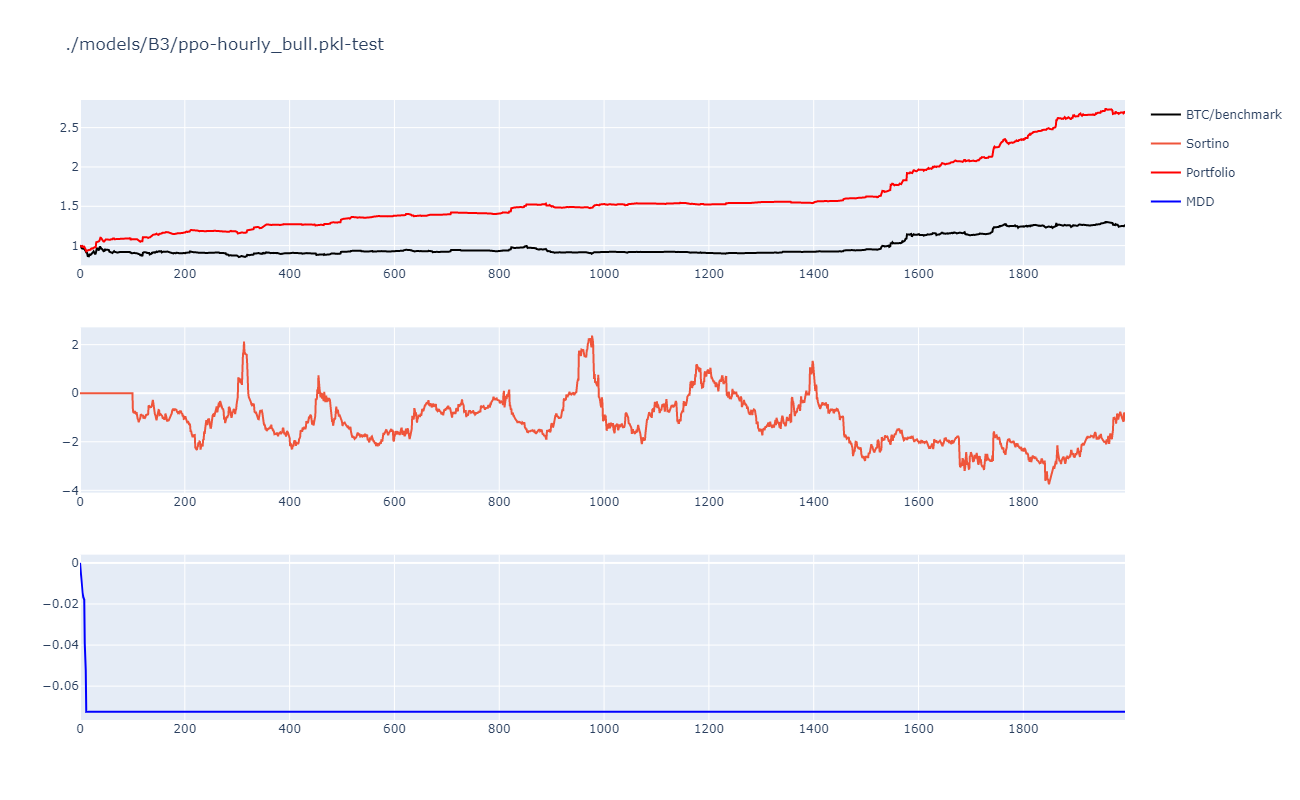
\includegraphics[width=0.94\textwidth]{graphics/testphoto/ppo-disc-hbu.png}
    \caption{Discrete PPO agent metrics for hourly bull data}
    \label{f-ppo-disc-hbu}
\end{figure}

\begin{figure}[H]
    \centering
    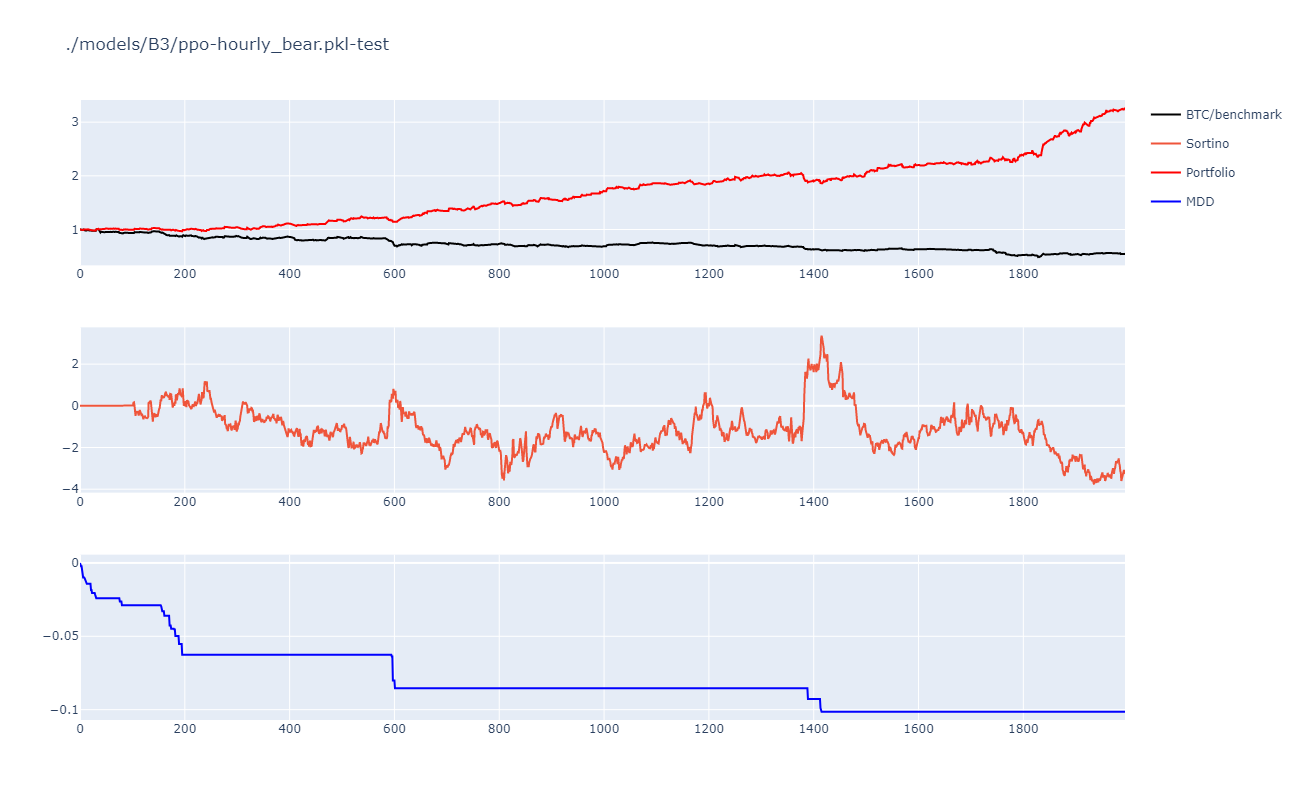
\includegraphics[width=0.94\textwidth]{graphics/testphoto/ppo-disc-hbr.png}
    \caption{Discrete PPO agent metrics for hourly bear data}
    \label{f-ppo-disc-hbr}
\end{figure}

\begin{figure}[H]
    \centering
    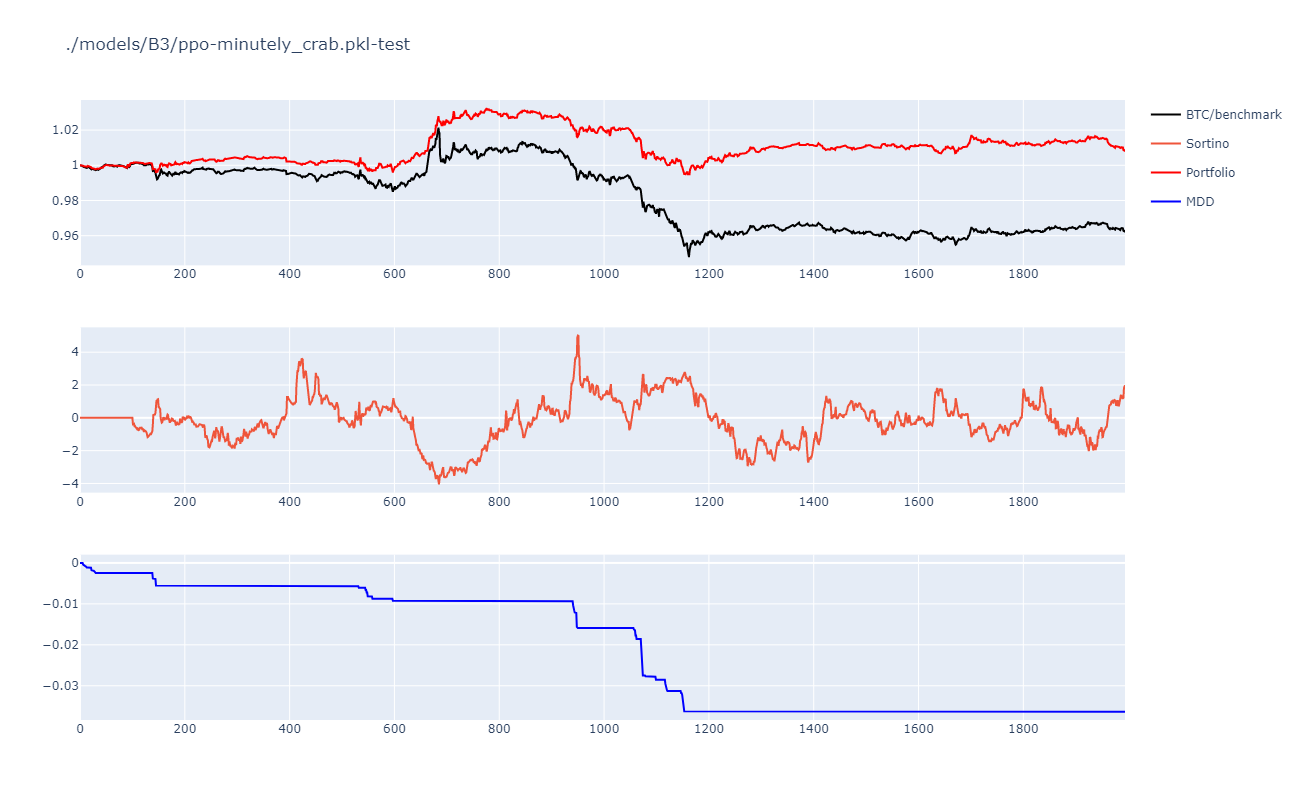
\includegraphics[width=0.94\textwidth]{graphics/testphoto/ppo-disc-mcr.png}
    \caption{Discrete PPO agent metrics for minute crab data}
    \label{f-ppo-disc-mcr}
\end{figure}

\begin{figure}[H]
    \centering
    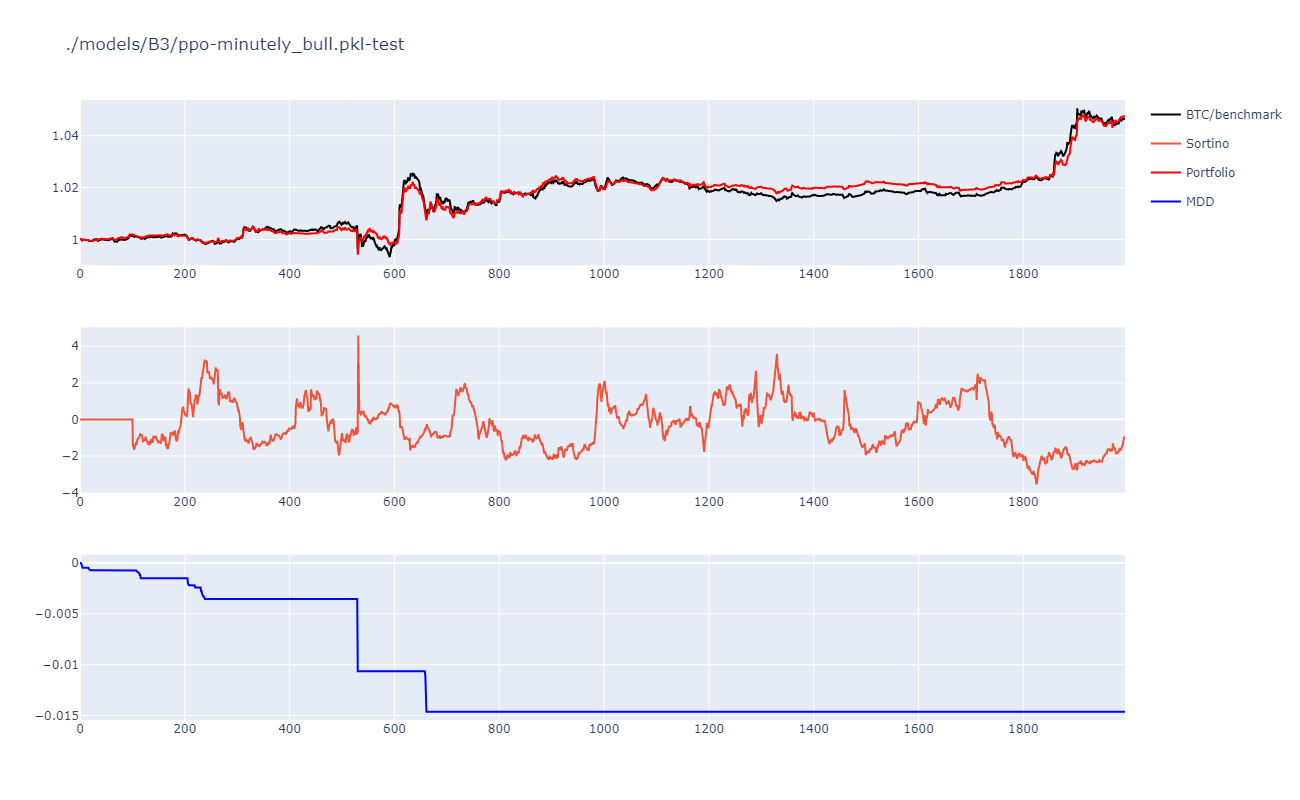
\includegraphics[width=0.94\textwidth]{graphics/testphoto/ppo-disc-mbu.png}
    \caption{Discrete PPO agent metrics for minute bull data}
    \label{f-ppo-disc-mbu}
\end{figure}

\subsection{PPO Strategy Agent (Continuous)}
This PPO agent is used with a continuous action space. The Continuous PPO agent results in more stable metrics over Discrete PPO, converging at around 1,800,000 timesteps ($\sim$167 episodes, $\sim$5,100 seconds) after having a peaking reward value at around 1,400,000 timesteps. Refer to Fig. \ref{gr:ppoc:train}.

\begin{figure}[H]
    \centering
    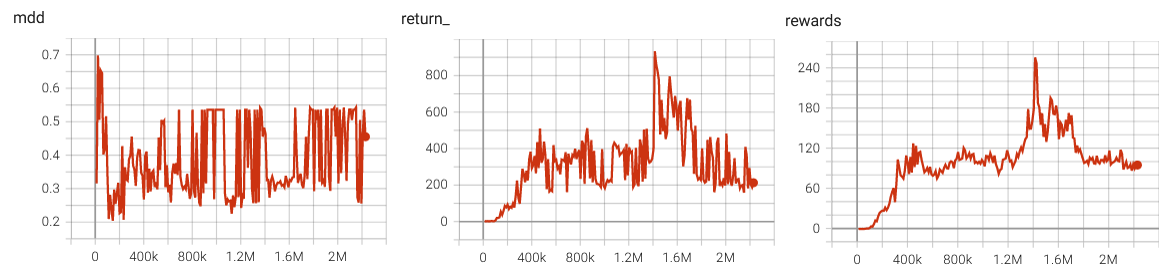
\includegraphics[width=0.99\textwidth]{graphics/trainphoto/ppoctrain.png}
    \caption{Continuous PPO Training Results}
    \label{gr:ppoc:train}
\end{figure}

Like Discrete PPO agent but less powerful, this Continuous PPO agent performs better than benchmark in all aspects, particularly the hourly datasets. An exception is the final return value for \texttt{MBu} dataset, where it performs 5.6\% lower than benchmark. See Table \ref{resl:cont-ppo}.

\begin{longtable}[c]{|l|rrr|rrr|r|c|}
\caption{Continuous PPO Test Results}
\label{resl:cont-ppo}\\
\hline
\multicolumn{1}{|c|}{\multirow{2}{*}{\textbf{$\mathcal{D}$}}} & \multicolumn{3}{c|}{\textbf{Agent}} & \multicolumn{3}{c|}{\textbf{Benchmark}} & \multicolumn{1}{c|}{\multirow{2}{*}{\textbf{$\overline{\Delta\phi_{\alpha,\odot}}$}}} & \multirow{2}{*}{\textbf{Fig.}} \\ \cline{2-7}
\multicolumn{1}{|c|}{} & \multicolumn{1}{c|}{\textbf{Return}} & \multicolumn{1}{c|}{\textbf{MDD}} & \multicolumn{1}{c|}{\textit{\textbf{Sortino}}} & \multicolumn{1}{c|}{\textbf{Return}} & \multicolumn{1}{c|}{\textbf{MDD}} & \multicolumn{1}{c|}{\textit{\textbf{Sortino}}} & \multicolumn{1}{c|}{} &  \\ \hline
\endfirsthead
%
\multicolumn{9}{c}%
{{\bfseries Table \thetable\ continued from previous page}} \\
\endhead
%
\textbf{\texttt{HBu}} & \multicolumn{1}{r|}{\textbf{0.6357}} & \multicolumn{1}{r|}{\textbf{0.0718}} & \textit{-1.2784} & \multicolumn{1}{r|}{0.2643} & \multicolumn{1}{r|}{0.1174} & \textit{0.7060} & 0.1897 & \ref{f-ppo-cont-hbu} \\ \hline
\textbf{\texttt{HBr}} & \multicolumn{1}{r|}{\textbf{0.2589}} & \multicolumn{1}{r|}{\textbf{0.1766}} & \textit{-1.6469} & \multicolumn{1}{r|}{-0.4484} & \multicolumn{1}{r|}{0.5199} & \textit{-0.3982} & 0.5571 & \ref{f-ppo-cont-hbr} \\ \hline
\textbf{\texttt{MCr}} & \multicolumn{1}{r|}{\textbf{-0.0265}} & \multicolumn{1}{r|}{\textbf{0.0551}} & \textit{2.0327} & \multicolumn{1}{r|}{-0.0361} & \multicolumn{1}{r|}{0.0725} & \textit{-0.2276} & 0.0057 & \ref{f-ppo-cont-mcr} \\ \hline
\textbf{\texttt{MBu}} & \multicolumn{1}{r|}{0.0416} & \multicolumn{1}{r|}{\textbf{0.0118}} & \textit{-0.0144} & \multicolumn{1}{r|}{\textbf{0.0441}} & \multicolumn{1}{r|}{0.0164} & \textit{1.0024} & 0.0017 & \ref{f-ppo-cont-mbu} \\ \hline
\end{longtable}


\begin{figure}[H]
    \centering
    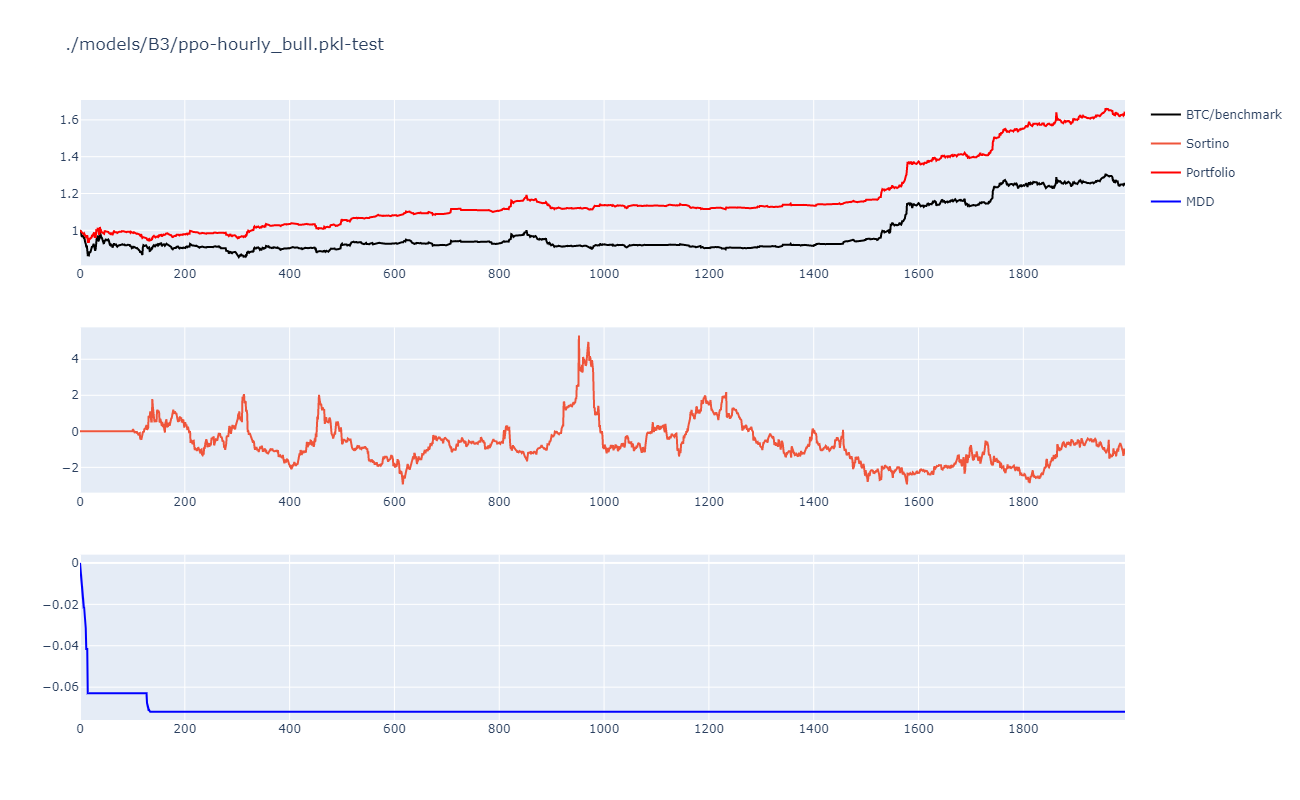
\includegraphics[width=0.94\textwidth]{graphics/testphoto/ppo-cont-hbu.png}
    \caption{Continuous PPO agent metrics for hourly bull data}
    \label{f-ppo-cont-hbu}
\end{figure}

\begin{figure}[H]
    \centering
    \includegraphics[width=0.94\textwidth]{graphics/testphoto/ppo-cont-hbr.png}
    \caption{Continuous PPO agent metrics for hourly bear data}
    \label{f-ppo-cont-hbr}
\end{figure}

\begin{figure}[H]
    \centering
    \includegraphics[width=0.94\textwidth]{graphics/testphoto/ppo-cont-mcr.png}
    \caption{Continuous PPO agent metrics for minute crab data}
    \label{f-ppo-cont-mcr}
\end{figure}

\begin{figure}[H]
    \centering
    \includegraphics[width=0.94\textwidth]{graphics/testphoto/ppo-cont-mbu.png}
    \caption{Continuous PPO agent metrics for minute bull data}
    \label{f-ppo-cont-mbu}
\end{figure}

\subsection{SAC Strategy Agent (Continuous)}
The SAC agent operates in the continuous action space. Unlike the other agents, the SAC agent takes approximately 10 times more training duration to complete one episode. Using early stopping, the representative model is taken from timestamp 1,080,968 (97th episode, $\sim$25,800 seconds). Refer to Fig. \ref{gr:sac:train}.

\begin{figure}[H]
    \centering
    \includegraphics[width=0.99\textwidth]{graphics/trainphoto/sac-train.png}
    \caption{SAC Training Results}
    \label{gr:sac:train}
\end{figure}

Despite the high reward and return values, on top of its longer training duration, the SAC agent performs similarly to the Continuous PPO agent, yet less satisfying. The SAC agent averages around 10–13\% higher than benchmark in hourly data, but rather equal to benchmark in minute data. However, this agent successfully dampens the maximum drawdown in all cases. See Table \ref{resl:-sac}.

\begin{longtable}[c]{|l|rrr|rrr|r|c|}
\caption{SAC Test Results}
\label{resl:-sac}\\
\hline
\multicolumn{1}{|c|}{\multirow{2}{*}{\textbf{$\mathcal{D}$}}} & \multicolumn{3}{c|}{\textbf{Agent}} & \multicolumn{3}{c|}{\textbf{Benchmark}} & \multicolumn{1}{c|}{\multirow{2}{*}{\textbf{$\overline{\Delta\phi_{\alpha,\odot}}$}}} & \multirow{2}{*}{\textbf{Fig.}} \\ \cline{2-7}
\multicolumn{1}{|c|}{} & \multicolumn{1}{c|}{\textbf{Return}} & \multicolumn{1}{c|}{\textbf{MDD}} & \multicolumn{1}{c|}{\textit{\textbf{Sortino}}} & \multicolumn{1}{c|}{\textbf{Return}} & \multicolumn{1}{c|}{\textbf{MDD}} & \multicolumn{1}{c|}{\textit{\textbf{Sortino}}} & \multicolumn{1}{c|}{} &  \\ \hline
\endfirsthead
%
\multicolumn{9}{c}%
{{\bfseries Table \thetable\ continued from previous page}} \\
\endhead
%
\textbf{\texttt{HBu}} & \multicolumn{1}{r|}{\textbf{0.3782}} & \multicolumn{1}{r|}{\textbf{0.0879}} & \textit{-1.1721} & \multicolumn{1}{r|}{0.2643} & \multicolumn{1}{r|}{0.1174} & \textit{0.7060} & 0.1097 & \ref{f-sac-hbu} \\ \hline
\textbf{\texttt{HBr}} & \multicolumn{1}{r|}{\textbf{-0.1993}} & \multicolumn{1}{r|}{\textbf{0.2915}} & \textit{-0.6846} & \multicolumn{1}{r|}{-0.4484} & \multicolumn{1}{r|}{0.5199} & \textit{-0.3982} & 0.1361 & \ref{f-sac-hbr} \\ \hline
\textbf{\texttt{MCr}} & \multicolumn{1}{r|}{\textbf{-0.0295}} & \multicolumn{1}{r|}{\textbf{0.0439}} & \textit{1.5296} & \multicolumn{1}{r|}{-0.0361} & \multicolumn{1}{r|}{0.0725} & \textit{-0.2276} & 0.0030 & \ref{f-sac-mcr} \\ \hline
\textbf{\texttt{MBu}} & \multicolumn{1}{r|}{0.0222} & \multicolumn{1}{r|}{\textbf{0.0105}} & \textit{-0.6082} & \multicolumn{1}{r|}{\textbf{0.0441}} & \multicolumn{1}{r|}{0.0164} & \textit{1.0024} & -0.0065 & \ref{f-sac-mbu} \\ \hline
\end{longtable}

\begin{figure}[H]
    \centering
    \includegraphics[width=0.94\textwidth]{graphics/testphoto/sac-hbu.png}
    \caption{SAC agent metrics for hourly bull data}
    \label{f-sac-hbu}
\end{figure}

\begin{figure}[H]
    \centering
    \includegraphics[width=0.94\textwidth]{graphics/testphoto/sac-hbr.png}
    \caption{SAC agent metrics for hourly bear data}
    \label{f-sac-hbr}
\end{figure}

\begin{figure}[H]
    \centering
    \includegraphics[width=0.94\textwidth]{graphics/testphoto/sac-mcr.png}
    \caption{SAC agent metrics for minute crab data}
    \label{f-sac-mcr}
\end{figure}

\begin{figure}[H]
    \centering
    \includegraphics[width=0.94\textwidth]{graphics/testphoto/sac-mbu.png}
    \caption{SAC agent metrics for minute bull data}
    \label{f-sac-mbu}
\end{figure}


\chapter{Discussion}
\label{ch:discussion}

\section{Results Summary}

Excluding Sortino, four factors can be used to comparing the ten agents: final return for each test dataset, MDD for each test dataset, average over benchmark for each test dataset, and training time in timesteps, episode, and seconds. Agents with continuous action space is marked by ``-C'' and discrete ``-D."

Table \ref{tab:agent-ret} shows the testing results based on the final results from different test datasets. Discrete PPO is by far leading in hourly data, while DQN leads when tested on \texttt{MCr}, and for \texttt{MBu}, the most profitable agent is Continuous A2C.

Discrete PPO and DQN's lead is confirmed by looking at the more general fact: average portfolio return over benchmark (Table \ref{tab:comp-over-bm}). In fact, DQN replaces Continuous A2C as the best agent for \texttt{MBu}, and the worst-performing agent is Continuous A2C, especially in hour-level data.

\begin{longtable}[c]{|r|rrrrrrrr|}
\caption{Agent Return Comparison}
\label{tab:agent-ret}\\
\hline
\multicolumn{1}{|c|}{\multirow{2}{*}{\textbf{$\mathcal{D}$}}} & \multicolumn{8}{c|}{\textbf{Return}} \\ \cline{2-9} 
\multicolumn{1}{|c|}{} & \multicolumn{1}{c|}{\textbf{Benchmark}} & \multicolumn{1}{c|}{\textbf{MACD}} & \multicolumn{1}{c|}{\textbf{DQN}} & \multicolumn{1}{c|}{\textbf{A2C-D}} & \multicolumn{1}{c|}{\textbf{A2C-C}} & \multicolumn{1}{c|}{\textbf{PPO-D}} & \multicolumn{1}{c|}{\textbf{PPO-C}} & \multicolumn{1}{c|}{\textbf{SAC}} \\ \hline
\endfirsthead
%
\multicolumn{9}{c}%
{{\bfseries Table \thetable\ continued from previous page}} \\
\endhead
%
\textbf{\texttt{HBu}} & \multicolumn{1}{l|}{0.2643} & \multicolumn{1}{l|}{0.2161} & \multicolumn{1}{r|}{0.1540} & \multicolumn{1}{r|}{0.2568} & \multicolumn{1}{r|}{0.0060} & \multicolumn{1}{r|}{\textbf{1.6982}} & \multicolumn{1}{r|}{0.6357} & 0.3782 \\ \hline
\textbf{\texttt{HBr}} & \multicolumn{1}{l|}{-0.4484} & \multicolumn{1}{l|}{-0.3389} & \multicolumn{1}{r|}{-0.1184} & \multicolumn{1}{r|}{-0.4543} & \multicolumn{1}{r|}{-0.4824} & \multicolumn{1}{r|}{\textbf{2.2585}} & \multicolumn{1}{r|}{0.2589} & -0.1993 \\ \hline
\textbf{\texttt{MCr}} & \multicolumn{1}{l|}{-0.0361} & \multicolumn{1}{l|}{-0.0148} & \multicolumn{1}{r|}{\textbf{0.0296}} & \multicolumn{1}{r|}{-0.0368} & \multicolumn{1}{r|}{-0.0137} & \multicolumn{1}{r|}{0.0090} & \multicolumn{1}{r|}{-0.0265} & -0.0295 \\ \hline
\textbf{\texttt{MBu}} & \multicolumn{1}{l|}{0.0441} & \multicolumn{1}{l|}{0.0364} & \multicolumn{1}{r|}{0.0357} & \multicolumn{1}{r|}{0.0462} & \multicolumn{1}{r|}{\textbf{0.0480}} & \multicolumn{1}{r|}{0.0475} & \multicolumn{1}{r|}{0.0416} & 0.0222 \\ \hline
\end{longtable}

\begin{longtable}[c]{|r|rrrrrrr|}
\caption{Return Over Benchmark Comparison}
\label{tab:comp-over-bm}\\
\hline
\multicolumn{1}{|c|}{\multirow{2}{*}{\textbf{$\mathcal{D}$}}} & \multicolumn{7}{c|}{\textbf{$\overline{\Delta\phi_{\alpha,\odot}}$}} \\ \cline{2-8} 
\multicolumn{1}{|c|}{} & \multicolumn{1}{c|}{\textbf{MACD}} & \multicolumn{1}{c|}{\textbf{DQN}} & \multicolumn{1}{c|}{\textbf{A2C-D}} & \multicolumn{1}{c|}{\textbf{A2C-C}} & \multicolumn{1}{c|}{\textbf{PPO-D}} & \multicolumn{1}{c|}{\textbf{PPO-C}} & \multicolumn{1}{c|}{\textbf{SAC}} \\ \hline
\endfirsthead
%
\multicolumn{8}{c}%
{{\bfseries Table \thetable\ continued from previous page}} \\
\endhead
%
\textbf{\texttt{HBu}} & \multicolumn{1}{r|}{0.0620} & \multicolumn{1}{r|}{0.0204} & \multicolumn{1}{r|}{0.0035} & \multicolumn{1}{r|}{-0.0602} & \multicolumn{1}{r|}{\textbf{0.5988}} & \multicolumn{1}{r|}{0.1897} & 0.1097 \\ \hline
\textbf{\texttt{HBr}} & \multicolumn{1}{r|}{0.1363} & \multicolumn{1}{r|}{0.3015} & \multicolumn{1}{r|}{-0.0009} & \multicolumn{1}{r|}{-0.0320} & \multicolumn{1}{r|}{\textbf{1.5396}} & \multicolumn{1}{r|}{0.5571} & 0.1361 \\ \hline
\textbf{\texttt{MCr}} & \multicolumn{1}{r|}{0.0118} & \multicolumn{1}{r|}{\textbf{0.0383}} & \multicolumn{1}{r|}{0.0000} & \multicolumn{1}{r|}{0.0168} & \multicolumn{1}{r|}{0.0287} & \multicolumn{1}{r|}{0.0057} & 0.0030 \\ \hline
\textbf{\texttt{MBu}} & \multicolumn{1}{r|}{-0.0008} & \multicolumn{1}{r|}{\textbf{0.0102}} & \multicolumn{1}{r|}{0.0000} & \multicolumn{1}{r|}{0.0023} & \multicolumn{1}{r|}{0.0006} & \multicolumn{1}{r|}{0.0017} & -0.0065 \\ \hline
\end{longtable}

The data about MDD aligns with all other findings except for \texttt{HBu}: for this particular case, Continuous PPO produces 1\% less drawdown than Discrete PPO. Overall, in most cases, RL agents tend to perform better in reducing drawdown than the plain buy-and-hold algorithm in minute level.

\begin{longtable}[c]{|l|rrrrrrrr|}
\caption{Agent MDD Comparison}
\label{tab:comp-mdd}\\
\hline
\multicolumn{1}{|c|}{\multirow{2}{*}{\textbf{$\mathcal{D}$}}} & \multicolumn{8}{c|}{\textbf{MDD}} \\ \cline{2-9} 
\multicolumn{1}{|c|}{} & \multicolumn{1}{c|}{\textbf{Benchmark}} & \multicolumn{1}{c|}{\textbf{MACD}} & \multicolumn{1}{c|}{\textbf{DQN}} & \multicolumn{1}{c|}{\textbf{A2C-D}} & \multicolumn{1}{c|}{\textbf{A2C-C}} & \multicolumn{1}{c|}{\textbf{PPO-D}} & \multicolumn{1}{c|}{\textbf{PPO-C}} & \multicolumn{1}{c|}{\textbf{SAC}} \\ \hline
\endfirsthead
%
\multicolumn{9}{c}%
{{\bfseries Table \thetable\ continued from previous page}} \\
\endhead
%
\textbf{\texttt{HBu}} & \multicolumn{1}{l|}{0.1174} & \multicolumn{1}{l|}{0.1159} & \multicolumn{1}{r|}{0.1812} & \multicolumn{1}{r|}{0.1425} & \multicolumn{1}{r|}{0.1622} & \multicolumn{1}{r|}{0.0725} & \multicolumn{1}{r|}{\textbf{0.0718}} & 0.0879 \\ \hline
\textbf{\texttt{HBr}} & \multicolumn{1}{l|}{0.5199} & \multicolumn{1}{l|}{0.3570} & \multicolumn{1}{r|}{0.1343} & \multicolumn{1}{r|}{0.5174} & \multicolumn{1}{r|}{0.5618} & \multicolumn{1}{r|}{\textbf{0.1014}} & \multicolumn{1}{r|}{0.1766} & 0.2915 \\ \hline
\textbf{\texttt{MCr}} & \multicolumn{1}{l|}{0.0725} & \multicolumn{1}{l|}{0.0427} & \multicolumn{1}{r|}{\textbf{0.0313}} & \multicolumn{1}{r|}{0.0719} & \multicolumn{1}{r|}{0.0462} & \multicolumn{1}{r|}{0.0363} & \multicolumn{1}{r|}{0.0551} & 0.0439 \\ \hline
\textbf{\texttt{MBu}} & \multicolumn{1}{l|}{0.0164} & \multicolumn{1}{l|}{0.0124} & \multicolumn{1}{r|}{\textbf{0.0061}} & \multicolumn{1}{r|}{0.0165} & \multicolumn{1}{r|}{0.0101} & \multicolumn{1}{r|}{0.0146} & \multicolumn{1}{r|}{0.0118} & 0.0105 \\ \hline
\end{longtable}

Lastly, it is undoubtably true that the buy-and-hold and MACD agents win the training time comparison, since they do not require any training to operate. Among RL algorithms, Discrete A2C only takes around 4,500 timesteps (4 episodes, 90 seconds) to find its ideal model, yet at the end it just mimics the buy-and-hold agent's performance. The second fastest model is DQN, with clear advantage when tested with minute-level test datasets. Continuous PPO converges before the episode limit (200 episodes), and results in a decent lead over benchmark. Discrete PPO and SAC failed to converge before the training episode limit (150 and 100, respecively), while it is difficult to tell if Continuous A2C would ever converge, due to its unstable nature.

\begin{longtable}[c]{|r|rrrrrr|}
\caption{Time Performance Comparison}
\label{tab:comp-time}\\
\hline
\multicolumn{1}{|c|}{\multirow{2}{*}{\textbf{}}} & \multicolumn{6}{c|}{\textit{\textbf{s}}} \\ \cline{2-7} 
\multicolumn{1}{|c|}{} & \multicolumn{1}{c|}{\textbf{DQN}} & \multicolumn{1}{c|}{\textbf{A2C-D}} & \multicolumn{1}{c|}{\textbf{A2C-C}} & \multicolumn{1}{c|}{\textbf{PPO-D}} & \multicolumn{1}{c|}{\textbf{PPO-C}} & \multicolumn{1}{c|}{\textbf{SAC}} \\ \hline
\endfirsthead
%
\multicolumn{7}{c}%
{{\bfseries Table \thetable\ continued from previous page}} \\
\endhead
%
\textbf{Timesteps} & \multicolumn{1}{r|}{768,936} & \multicolumn{1}{r|}{\textbf{$\sim$45,000}} & \multicolumn{1}{r|}{> 1,671,600} & \multicolumn{1}{r|}{> 2,228,800} & \multicolumn{1}{r|}{$\sim$1,800,000} & > 1,114,400 \\ \hline
\textbf{Episodes} & \multicolumn{1}{r|}{69} & \multicolumn{1}{r|}{\textbf{4}} & \multicolumn{1}{r|}{> 150} & \multicolumn{1}{r|}{> 200} & \multicolumn{1}{r|}{$\sim$167} & > 100 \\ \hline
\textbf{Time} & \multicolumn{1}{r|}{$\sim$2,500} & \multicolumn{1}{r|}{\textbf{$\sim$90}} & \multicolumn{1}{r|}{> 5,500} & \multicolumn{1}{r|}{> 5,000} & \multicolumn{1}{r|}{$\sim$5,100} & > 25,800 \\ \hline
\end{longtable}

\section{Findings}
(to be completed)

\section{Shortcomings}
(to be completed)

\section{Recommendations}
(to be completed)
\chapter{Conclusion}
\label{Conclusion}

\section{Summary}
\section{Strengths and Shortcomings}

\begin{appendix}
\chapter{Symbols and Variables}
    \label{appx:label1}
   
    \begin{longtable}{p{2.2cm}|p{2cm}|p{9cm}}
	\caption{List of Symbols}
		\endfirsthead
		\caption[]{List of Symbols (continued)}\\
		\endhead

	\label{app-symbol}
	\textbf{Symbol} & \textbf{Scope} & \textbf{Meaning} \\ \hline
	$\mathcal{D}$ & general & dataset \\
	$\delta_t$ & general & data point at timeframe $t$ \\
	$p_t$ & general & closing price at timeframe $t$ \\
	$EMA(n)$ & indicator & exponential moving average with window size $n$ \\
	$MACD(f, s, l)$ & indicator & movement average convergence/divergence of fast linie period $f$, slow line period $s$, and signal line period $l$ \\
	$\phi(a)_t$ & portfolio & portfolio size of asset $a$ at timeframe $t$ \\
	$\phi_\odot$ & portfolio & benchmark (buy-and-hold) portfolio return \\
	$\overline{\Delta\phi_{\alpha,\beta}}$ & portfolio & difference between portfolio returns given by agent $\alpha$ and agent $\beta$ \\
	$MDD_t$ & portfolio & maximum drawdown at timeframe $t$ \\
	$\zeta_t$ & portfolio & Sortino ratio at timeframe $t$ \\
	$s$ & agent & approximate time for an agent's training reward value to converge\\

	\end{longtable}

\end{appendix}

% \begin{thebibliography}{1}

% \bibitem{IEEEhowto:kopka}
% H.~Kopka and P.~W. Daly, \emph{A Guide to \LaTeX}, 3rd~ed.\hskip 1em plus
%   0.5em minus 0.4em\relax Harlow, England: Addison-Wesley, 1999.



\bibitem{bib:backpain}
C. Gent, J. Dols, C. Rover, R. Sing and H. Vet, "Heavy Bags Lead to Back Pain in Children", Medscape, 2003. [Online]. Available: http://www.medscape.com/viewarticle/455563\_4. [Accessed: 04- May- 2016].

\bibitem{bib:What is NFC}
  "What Is NFC? - NFC Forum", NFC Forum, 2016. [Online]. Available: http://nfc-forum.org/what-is-nfc/. [Accessed: 04-May-2016].

\bibitem{bib:NFC_bootstrapping}
"NFC Forum: NFC as Technology Enabler", NFC Forum. [Online]. Available: http://members.nfc-forum.org/aboutnfc/tech\_enabler/. [Accessed: 18- May- 2016].

\bibitem{bib:NFC Phones List}
"List of NFC phones", NFC World+, 2016. [Online]. Available: http://www.nfcworld.com/nfc-phones-list/. [Accessed: 04-May- 2016].

\bibitem{bib:Chromecast}
  "Chromecast - Google", Google.com, 2016. [Online]. Available: https://www.google.com/chromecast. [Accessed: 04-May-2016].
  
\bibitem{bib:UPnP Device Architecture}
  UPnP Forum, "UPnP™ Device Architecture 1.1", 2008. 
  
\bibitem{bib:FSPL}
J. Yang and Y. Chen, "Indoor Localization Using Improved RSS-Based Lateration Methods," Global Telecommunications Conference, 2009. GLOBECOM 2009. IEEE, Honolulu, HI, 2009, pp. 1-6.

\bibitem{bib:ARP}
D. Plummer, "RFC 826 - Ethernet Address Resolution Protocol: Or Converting Network Protocol Addresses to 48.bit Ethernet Address for Transmission on Ethernet Hardware", 1982. [Online]. Available: https://tools.ietf.org/html/rfc826. [Accessed: 18- May- 2016].

\bibitem{bib:ARP Timeout}
"arp(7): ARP kernel module - Linux man page", Linux.die.net. [Online]. Available: http://linux.die.net/man/7/arp. [Accessed: 04-May-2016].

\bibitem{bib:bluetooth_vs_wifi}
Mautz, R., 2012. Indoor positioning technologies (Doctoral dissertation, Habilitationsschrift ETH Zürich, 2012).

\bibitem{bib:distance_with_RSSI}
J. Rogowski, "Distance measurement using radio frequency identification technology," Scientific and Technical Conference "Computer Sciences and Information Technologies" (CSIT), 2015 Xth International, Lviv, 2015, pp. 9-15.
doi: 10.1109/STC-CSIT.2015.7325420
keywords: {radiofrequency identification;asset localisation applicable format;competitive product;distance measurement;radio frequency identification technology;real-time localisation system;Accuracy;Algorithm design and analysis;Antennas;Calibration;Radiofrequency identification;Real-time systems;Receivers;RFID;asset localisation system},
URL: http://ieeexplore.ieee.org/stamp/stamp.jsp?tp=\&arnumber=7325420\&isnumber=7325415

\bibitem{bib:rssi_reliability}
Qian Dong and W. Dargie, "Evaluation of the reliability of RSSI for indoor localization," Wireless Communications in Unusual and Confined Areas (ICWCUCA), 2012 International Conference on, Clermont Ferrand, 2012, pp. 1-6.
doi: 10.1109/ICWCUCA.2012.6402492
URL: http://ieeexplore.ieee.org/stamp/stamp.jsp?tp=\&arnumber=6402492\&isnumber=6402322

\bibitem{bib:timeofflight}
L. Schauer, F. Dorfmeister and M. Maier, "Potentials and limitations of WIFI-positioning using Time-of-Flight," Indoor Positioning and Indoor Navigation (IPIN), 2013 International Conference on, Montbeliard-Belfort, 2013, pp. 1-9.
doi: 10.1109/IPIN.2013.6817861
URL: http://ieeexplore.ieee.org/stamp/stamp.jsp?tp=\&arnumber=6817861\&isnumber=6817839

\bibitem{bib:Chronos}
D.  Vasisht, S.  Kumar and D.  Katabi, "Decimeter-Level Localization with a Single WiFi Access Point", in 13th USENIX Symposium on Networked Systems Design and Implementation (NSDI 16), 2016, pp. 165-178.

\end{thebibliography}

%\renewcommand\bibname{References}
\addcontentsline{toc}{chapter}{References}
\bibliographystyle{IEEEtran}
% \bibliographystyle{unsrt}
% \bibliographystyle{unsrt}
% \bibliographystyle{plainnat} % or try abbrvnat or unsrtnat
% \nocite{*}
\bibliography{misc/bibliography.bib}

\end{document}